% ============================================================
%  يُترجَم بـ XeLaTeX  (في Overleaf: Menu → Compiler → XeLaTeX)
%  الخط: Amiri (متوفر في Overleaf، أو حمّله من github.com/aliftype/amiri)
% ============================================================
\documentclass[12pt,a4paper]{article}
\usepackage[a4paper,margin=1.7cm,top=2.3cm,bottom=2.9cm,headheight=15pt,footskip=1.5cm]{geometry}
\usepackage{amsmath,amssymb}
\usepackage{icomma}
\usepackage[english,bidi=default,layout=lists]{babel}
\babelprovide[import,main]{arabic}
\babelfont{rm}[Scale=1.08]{Amiri}
\babelfont{sf}[Scale=1.08]{Amiri}
\usepackage[most]{tcolorbox}
\usepackage{tikz}
\usetikzlibrary{arrows.meta,calc,shadings}
\usepackage{array}
\usepackage{colortbl}
\usepackage{fancyhdr}
\usepackage{titlesec}
\usepackage{enumitem}
\usepackage{collcell}
\usepackage{needspace}
\usepackage{etoolbox}
\newcolumntype{C}{>{\collectcell\ar}c<{\endcollectcell}}
\pretocmd{\section}{\Needspace{15\baselineskip}}{}{}
\pretocmd{\subsection}{\Needspace{11\baselineskip}}{}{}

\definecolor{cDef}{HTML}{1F4E9C}
\definecolor{cThm}{HTML}{B3261E}
\definecolor{cRem}{HTML}{2E7D32}
\definecolor{cEx}{HTML}{C76B00}
\definecolor{cMeth}{HTML}{6A1B9A}
\definecolor{cSol}{HTML}{00695C}
\definecolor{cSec}{HTML}{1F3A68}

\titleformat{\section}{\Large\bfseries\color{cSec}}{\thesection.}{0.6em}{}[{\color{cSec!60}\titlerule[1pt]}]
\titleformat{\subsection}{\large\bfseries\color{cThm!85!black}}{\thesubsection.}{0.5em}{}
\titlespacing*{\section}{0pt}{14pt}{8pt}
\titlespacing*{\subsection}{0pt}{10pt}{5pt}
\setlength{\parindent}{0pt}
\setlength{\parskip}{4pt}
\setlist{itemsep=2pt,topsep=3pt}

\newtcolorbox{arbox}[3][]{enhanced,
  colback=#2!5,colframe=#2!80!black,arc=2mm,boxrule=0.8pt,
  left=6pt,right=6pt,top=8pt,bottom=5pt,
  fonttitle=\bfseries,coltitle=white,
  title={\foreignlanguage{arabic}{#3}},
  attach boxed title to top right={xshift=-5mm,yshift=-3mm},
  boxed title style={colback=#2!80!black,arc=1.5mm,boxrule=0pt},
  before upper={\selectlanguage{arabic}},
  before skip=8pt,after skip=8pt,breakable,#1}
\newenvironment{BOX}[2]{\begin{otherlanguage}{english}\begin{arbox}{#1}{#2}}{\end{arbox}\end{otherlanguage}}
\newenvironment{tarif}[1][تعريف]{\begin{BOX}{cDef}{#1}}{\end{BOX}}
\newenvironment{khassia}[1][خاصية]{\begin{BOX}{cThm}{#1}}{\end{BOX}}
\newenvironment{molahada}[1][ملاحظة]{\begin{BOX}{cRem}{#1}}{\end{BOX}}
\newenvironment{mithal}[1][مثال]{\begin{BOX}{cEx}{#1}}{\end{BOX}}
\newenvironment{tariqa}[1][طريقة]{\begin{BOX}{cMeth}{#1}}{\end{BOX}}

\newcounter{exo}
\newenvironment{tamrin}[1]{\stepcounter{exo}\begin{BOX}{cSec}{التمرين \theexo: #1}}{\end{BOX}}
\newenvironment{hal}{\Needspace{12\baselineskip}\begin{otherlanguage}{english}\begin{arbox}[breakable]{cSol}{حل التمرين \theexo}}{\end{arbox}\end{otherlanguage}}

\newenvironment{LTR}{\begin{otherlanguage}{english}}{\end{otherlanguage}}
\newcommand{\ar}[1]{\foreignlanguage{arabic}{#1}}

\renewcommand{\dots}{\mathinner{\ldotp\ldotp\ldotp}}
\renewcommand{\ldots}{\mathinner{\ldotp\ldotp\ldotp}}
\renewcommand{\cdots}{\mathinner{\cdotp\cdotp\cdotp}}
\newcommand{\N}{\mathbb{N}}
\newcommand{\Z}{\mathbb{Z}}
\newcommand{\D}{\mathbb{D}}
\newcommand{\Q}{\mathbb{Q}}
\newcommand{\R}{\mathbb{R}}
\newcommand{\pgcd}{\operatorname{PGCD}}
\newcommand{\ppcm}{\operatorname{PPCM}}

% \NLseg{a}{b}{[}{]} ; \NLright{a}{[} ; \NLleft{b}{]}  (interval on a number line)
\newcommand{\NLseg}[4]{\begin{LTR}\begin{tikzpicture}[baseline=-0.6ex]
 \draw[-{Stealth[length=2mm]},gray!70](0,0)--(3.4,0);
 \draw[line width=2pt,cThm!80!black](0.7,0)--(2.7,0);
 \node[cThm!80!black,font=\LARGE] at (0.7,0){$#3$};
 \node[cThm!80!black,font=\LARGE] at (2.7,0){$#4$};
 \node[below=3pt,font=\footnotesize] at (0.7,0){$#1$};
 \node[below=3pt,font=\footnotesize] at (2.7,0){$#2$};
\end{tikzpicture}\end{LTR}}
\newcommand{\NLright}[2]{\begin{LTR}\begin{tikzpicture}[baseline=-0.6ex]
 \draw[-{Stealth[length=2mm]},gray!70](0,0)--(3.4,0);
 \draw[line width=2pt,cThm!80!black](1.3,0)--(3.3,0);
 \node[cThm!80!black,font=\LARGE] at (1.3,0){$#2$};
 \node[below=3pt,font=\footnotesize] at (1.3,0){$#1$};
\end{tikzpicture}\end{LTR}}
\newcommand{\NLleft}[2]{\begin{LTR}\begin{tikzpicture}[baseline=-0.6ex]
 \draw[-{Stealth[length=2mm]},gray!70](0,0)--(3.4,0);
 \draw[line width=2pt,cThm!80!black](0.05,0)--(2.1,0);
 \node[cThm!80!black,font=\LARGE] at (2.1,0){$#2$};
 \node[below=3pt,font=\footnotesize] at (2.1,0){$#1$};
\end{tikzpicture}\end{LTR}}

% ---------- social-media icons (pure TikZ) ----------
\definecolor{cFB}{HTML}{1877F2}
\definecolor{cTG}{HTML}{229ED9}
\definecolor{cIG1}{HTML}{FEDA75}
\definecolor{cIG2}{HTML}{D62976}
\definecolor{cIG3}{HTML}{4F5BD5}
\newcommand{\fbicon}{\begin{LTR}\begin{tikzpicture}[baseline=-0.75ex,x=1em,y=1em]
 \fill[cFB] (0,0) circle (0.55);
 \node[white,inner sep=0,font=\usefont{TU}{lmss}{bx}{n}\small] at (0.04,-0.02) {f};
\end{tikzpicture}\end{LTR}}
\newcommand{\igicon}{\begin{LTR}
\begin{tikzpicture}[baseline=-0.75ex,x=1em,y=1em]
 \shade[lower left=cIG1,lower right=cIG2,upper left=cIG2,upper right=cIG3,rounded corners=0.28em] (-0.55,-0.55) rectangle (0.55,0.55);
 \draw[white,line width=0.09em,rounded corners=0.18em] (-0.36,-0.36) rectangle (0.36,0.36);
 \draw[white,line width=0.09em] (0,0) circle (0.17);
 \fill[white] (0.22,0.22) circle (0.05);
\end{tikzpicture}\end{LTR}}
\newcommand{\tgicon}{\begin{LTR}
\begin{tikzpicture}[baseline=-0.75ex,x=1em,y=1em]
 \fill[cTG] (0,0) circle (0.55);
 \fill[white] (-0.33,0.0) -- (0.32,0.27) -- (0.2,-0.3) -- (0.0,-0.15) -- (-0.08,-0.28) -- (-0.08,-0.08) -- cycle;
 \fill[cTG!70!black] (-0.08,-0.08) -- (0.25,0.2) -- (0.0,-0.15) -- (-0.08,-0.28) -- cycle;
\end{tikzpicture}\end{LTR}}
% page number: black box, white two-digit number, at the right of the social row
\newcommand{\PageBox}{\begin{LTR}\tikz[baseline=(p.base)]\node[fill=black,text=white,inner sep=2.5pt,minimum width=1.6em,minimum height=1.3em,font=\usefont{TU}{lmss}{bx}{n}\small](p){\ifnum\value{page}<10 0\fi\arabic{page}};\end{LTR}}
% visual left-to-right order: Telegram | Instagram | Facebook | page box
\newcommand{\SocialRow}{\begin{otherlanguage}{english}%
 \ar{\textbf{الأستاذ سوايسية هشام للرياضيات}}\ \tgicon\hfill
 \textbf{prof\_hicham\_math}\ \igicon\hfill
 \ar{\textbf{الأستاذ سوايسية هشام للرياضيات}}\ \fbicon\hspace{2.2em}\PageBox\end{otherlanguage}}

\pagestyle{fancy}
\fancyhf{}
\renewcommand{\headrulewidth}{0.6pt}
\renewcommand{\footrulewidth}{0.4pt}
% \SetHeader{right head: document title}{left head: level -- stream}
\newcommand{\SetHeader}[2]{%
 \fancyhead[C]{\parbox{\textwidth}{\ar{#1\hfill #2}}}%
 \fancyfoot[C]{\parbox{\textwidth}{\small\SocialRow}}}
\usepackage{tkz-tab}
\usepackage{multicol}
% variation / sign table (LTR)
\newenvironment{TAB}{\par\begin{center}\begin{LTR}\begin{tikzpicture}[scale=0.95,every node/.style={font=\small}]}{\end{tikzpicture}\end{LTR}\end{center}}
% grid + axes, clipped: \begin{GR}{xmin}{xmax}{ymin}{ymax}{unit cm}
\newenvironment{GR}[5]{\par\begin{center}\begin{LTR}\begin{tikzpicture}[x=#5cm,y=#5cm,font=\footnotesize]
 \draw[gray!25,very thin] (#1,#3) grid (#2,#4);
 \draw[-{Stealth[length=2mm]}] (#1,0)--(#2+0.3,0) node[below left]{$x$};
 \draw[-{Stealth[length=2mm]}] (0,#3)--(0,#4+0.3) node[below left]{$y$};
 \node[below left] at (0,0){$O$};
 \begin{scope}\clip (#1,#3) rectangle (#2,#4);}
{\end{scope}\end{tikzpicture}\end{LTR}\end{center}}
\newcommand{\Ticks}[2]{\foreach \t in {#1} \node[below,font=\scriptsize] at (\t,0){$\t$}; \foreach \t in {#2} \node[left,font=\scriptsize] at (0,\t){$\t$};}
\newcommand{\bx}[1]{\ensuremath{\colorbox{cDef!12}{$\displaystyle #1$}}}
\newcommand{\TwoCol}[4]{\par\begin{LTR}\noindent\begin{minipage}[t]{#1\textwidth}\selectlanguage{arabic}#2\end{minipage}\hfill\begin{minipage}[t]{#3\textwidth}\selectlanguage{arabic}#4\end{minipage}\end{LTR}\par}
\newcommand{\RL}[4]{\TwoCol{#3}{#4}{#1}{#2}}  % \RL{w1}{right content}{w2}{left content}
\newcommand{\ok}{$\textcolor{cRem}{\checkmark}$}
\newcommand{\limn}{\displaystyle\lim_{n\to+\infty}}
% sub-questions, each on its own line
\newenvironment{sq}{\begin{itemize}[leftmargin=2.4em,itemsep=3pt]}{\end{itemize}}
\newcommand{\qa}{\item[(أ)]}\newcommand{\qb}{\item[(ب)]}\newcommand{\qc}{\item[(جـ)]}\newcommand{\qd}{\item[(د)]}\newcommand{\qe}{\item[(هـ)]}
\newcommand{\pa}{\par\smallskip\textbf{(أ)} }\newcommand{\pb}{\par\smallskip\textbf{(ب)} }\newcommand{\pc}{\par\smallskip\textbf{(جـ)} }\newcommand{\pd}{\par\smallskip\textbf{(د)} }\newcommand{\pe}{\par\smallskip\textbf{(هـ)} }
\newcommand{\QQ}[1]{\par\smallskip\textbf{#1.} }
\newenvironment{tmr}{\stepcounter{exo}\begin{BOX}{cSec}{تمرين محلول \theexo}}{\end{BOX}}
\newcommand{\ABC}[3]{\\[2pt]\begin{tabular}{p{0.28\textwidth}p{0.28\textwidth}p{0.28\textwidth}}(جـ) \ #3 & (ب) \ #2 & (أ) \ #1\end{tabular}}
\pretocmd{\section}{\Needspace{24\baselineskip}}{}{}
\newtcbox{\bxtbox}{on line,colback=cDef!12,colframe=cDef!12,boxrule=0pt,arc=1pt,boxsep=0pt,left=2pt,right=2pt,top=1pt,bottom=1pt}
\newcommand{\bxt}[1]{\foreignlanguage{english}{\bxtbox{\ar{#1}}}}
\SetHeader{\small\bfseries\color{cSec}تمارين البكالوريا: الأعداد والحساب}{\small\color{cSec}السنة الثالثة ثانوي -- رياضيات وتقني رياضي}
\begin{document}
\begin{LTR}
\begin{tcolorbox}[enhanced,colback=cSec,colframe=cSec,arc=3mm,halign=center,boxrule=0pt,top=12pt,bottom=12pt,before upper={\selectlanguage{arabic}}]
{\color{white}\fontsize{26}{32}\selectfont\bfseries تمارين البكالوريا في الأعداد والحساب}\\[8pt]
{\color{white}\large مع الحلول المفصلة -- حتى دورة 2026}\\[5pt]
{\color{white}\large شعبة رياضيات -- شعبة تقني رياضي}
\end{tcolorbox}
\end{LTR}
\section{تمارين البكالوريا -- شعبة رياضيات}
% ================= التمرين: بكالوريا 2026 م1 =================
\begin{tamrin}{بكالوريا 2026 -- الموضوع الأول -- شعبة رياضيات}
نعتبر المعادلة $(E)$: \quad $675x-525y=\alpha$ حيث $x$ و $y$ عددان صحيحان و $\alpha$ عدد صحيح غير معدوم.

\textbf{1)} عيّن القاسم المشترك الأكبر للعددين $675$ و $525$ ثم استنتج قيم $\alpha$ التي تقبل من أجلها المعادلة $(E)$ حلولا.

\textbf{2)} نضع: $\alpha=825$.
\begin{sq}
\qa حلّ المعادلة $(E)$ علما أن الثنائية $(2;1)$ حل لها.
\qb عيّن كل الثنائيات $(x;y)$ حلول المعادلة $(E)$ التي من أجلها يكون: $\pgcd(x;y)=11$.
\end{sq}
\textbf{3)}
\begin{sq}
\qa أثبت أنه من أجل كل عدد طبيعي $n$ فإن العددين $7n+4$ و $9n+5$ أوليان فيما بينهما.
\qb أحسب بدلالة العدد الطبيعي غير المعدوم $n$ القاسم المشترك الأكبر والمضاعف المشترك الأصغر للعددين $a$ و $b$ حيث: $a=77n^2+44n$ و $b=99n^2+55n$.
\end{sq}
\textbf{4)}
\begin{sq}
\qa أدرس تبعا لقيم العدد الطبيعي $n$ بواقي القسمة الإقليدية للعدد $4^n$ على $7$.
\qb استنتج باقي القسمة الإقليدية للعدد $L$ على $7$ حيث: $L=1+2+2^2+\cdots+2^{2025}$.
\end{sq}
\textbf{5)} عيّن قيم العدد الطبيعي $n$ التي من أجلها يكون: $L+b-a+3\equiv 0\,[7]$.
\end{tamrin}
\begin{hal}
\QQ{1} \textbf{حساب} $\pgcd(675;525)$ \textbf{بخوارزمية إقليدس:}
\[675=1\times 525+150,\qquad 525=3\times150+75,\qquad 150=2\times 75+0.\]
آخر باقٍ غير معدوم هو $75$، إذن: \bx{\pgcd(675;525)=75}.

\textbf{شرط وجود الحلول:} المعادلة $ax+by=c$ تقبل حلولا في $\Z^2$ إذا وفقط إذا كان $\pgcd(a;b)$ يقسم $c$.
إذن $(E)$ تقبل حلولا إذا وفقط إذا كان $75\mid\alpha$، أي:
\bxt{$\alpha=75k$ حيث $k\in\Z^*$} (لأن $\alpha\neq0$).

\QQ{2} \pa لدينا $825=75\times 11$، فبالقسمة على $75$ تصبح المعادلة: $9x-7y=11$.

التحقق: $9\times2-7\times1=18-7=11$، إذن $(2;1)$ حل خاص.

بالطرح: $9x-7y=11$ و $9\times2-7\times1=11$ ومنه $9(x-2)=7(y-1)$.

$7$ يقسم $9(x-2)$ و $\pgcd(7;9)=1$، إذن حسب مبرهنة \textbf{غوص}: $7$ يقسم $x-2$، أي $x-2=7k$ مع $k\in\Z$.

بالتعويض: $9\times 7k=7(y-1)$ ومنه $y-1=9k$.

إذن حلول المعادلة $(E)$ هي: \bx{(x;y)=(7k+2\,;\,9k+1),\quad k\in\Z}.

\pb ليكن $d=\pgcd(x;y)$. بما أن $d\mid x$ و $d\mid y$ فإن $d\mid 9x-7y$ أي $d\mid 11$، و $11$ أولي، إذن $d\in\{1;11\}$.

$d=11$ يكافئ $11\mid x$ و $11\mid y$. لكن إذا كان $11\mid x$ فإن $7y=9x-11$ يقبل القسمة على $11$، و $\pgcd(7;11)=1$ إذن $11\mid y$ (غوص). يكفي إذن أن يكون $11\mid x$:
\[7k+2\equiv0\,[11]\iff 7k\equiv-2\equiv 9\,[11].\]
نضرب في $8$ (لأن $7\times8=56\equiv1\,[11]$): $k\equiv 72\equiv 6\,[11]$، أي $k=11m+6$ مع $m\in\Z$.

بالتعويض: $x=7(11m+6)+2=77m+44$ و $y=9(11m+6)+1=99m+55$.

إذن: \bx{(x;y)=(77m+44\,;\,99m+55),\quad m\in\Z}.

\QQ{3} \pa ليكن $\delta=\pgcd(7n+4;9n+5)$. $\delta$ يقسم كل تركيبة خطية منهما، ولدينا:
\[9(7n+4)-7(9n+5)=63n+36-63n-35=1.\]
إذن $\delta\mid 1$ ومنه $\delta=1$: \bxt{$7n+4$ و $9n+5$ أوليان فيما بينهما}.

\pb نحلّل: $a=77n^2+44n=11n(7n+4)$ و $b=99n^2+55n=11n(9n+5)$.

بما أن $\pgcd(ka;kb)=k\,\pgcd(a;b)$ من أجل $k\in\N^*$:
\[\pgcd(a;b)=11n\cdot\pgcd(7n+4;9n+5)=11n\times 1.\]
إذن \bx{\pgcd(a;b)=11n}.

ومن العلاقة $\pgcd(a;b)\times\ppcm(a;b)=a\times b$:
\[\ppcm(a;b)=\frac{11n(7n+4)\times 11n(9n+5)}{11n}=11n(7n+4)(9n+5).\]
إذن \bx{\ppcm(a;b)=11n(7n+4)(9n+5)}.

\QQ{4} \pa نحسب: $4^0=1$، $4^1=4$، $4^2=16\equiv2\,[7]$، $4^3=64\equiv1\,[7]$.

بما أن $4^3\equiv1\,[7]$ فإن البواقي دورية ودورها $3$: من أجل $k\in\N$:
$4^{3k}=(4^3)^k\equiv1$، $4^{3k+1}\equiv4$، $4^{3k+2}\equiv 2\,[7]$.
\begin{center}
\begin{tabular}{|>{\centering\arraybackslash}m{3.3cm}|c|c|c|}\hline
$n$ & $3k$ & $3k+1$ & $3k+2$\\\hline
باقي قسمة $4^n$ على $7$ & $1$ & $4$ & $2$\\\hline
\end{tabular}
\end{center}

\pb $L$ مجموع حدود متتابعة لمتتالية هندسية أساسها $2$ وحدها الأول $1$، عدد حدودها $2026$:
\[L=\frac{2^{2026}-1}{2-1}=2^{2026}-1=(2^2)^{1013}-1=4^{1013}-1.\]
لدينا $1013=3\times337+2$ إذن $4^{1013}\equiv2\,[7]$ ومنه $L\equiv 2-1=1\,[7]$.

إذن: \bxt{باقي قسمة $L$ على $7$ هو $1$}.

\QQ{5} لدينا $b-a=(99-77)n^2+(55-44)n=22n^2+11n$. وبما أن $22\equiv1\,[7]$ و $11\equiv4\,[7]$:
\[L+b-a+3\equiv 1+n^2+4n+3=n^2+4n+4=(n+2)^2\,[7].\]
إذن: $L+b-a+3\equiv0\,[7]\iff 7\mid (n+2)^2$. وبما أن $7$ أولي، فإن $7\mid(n+2)^2$ يكافئ $7\mid n+2$، أي $n\equiv-2\equiv5\,[7]$.

إذن: \bx{n=7k+5,\quad k\in\N}.
\end{hal}

% ================= بكالوريا 2026 م2 =================
\begin{tamrin}{بكالوريا 2026 -- الموضوع الثاني -- شعبة رياضيات}
المستوي منسوب إلى المعلم المتعامد والمتجانس $(O;\vec i,\vec j)$.
$ABC$ مثلث قائم في $A$ حيث: $A(6;9)$، $B(\alpha;0)$ و $C(0;\beta)$، $\alpha$ و $\beta$ عددان صحيحان.

\textbf{1)} بيّن أن الثنائية $(\alpha;\beta)$ تحقق المعادلة: $(E)$:\quad $2x+3y=39$، حيث $x$ و $y$ عددان صحيحان.

\textbf{2)}
\begin{sq}
\qa تحقق أن الثنائية $(6;9)$ حل للمعادلة $(E)$، ثم عيّن كل الثنائيات $(x;y)$ حلول المعادلة $(E)$.
\qb استنتج كل الثنائيات $(x;y)$ حلول المعادلة $(E)$ حيث: $\pgcd(x;y)=39$.
\end{sq}
\textbf{3)}
\begin{sq}
\qa أدرس حسب قيم العدد الطبيعي $n$ بواقي القسمة الإقليدية للعدد $4^n$ على $9$.
\qb استنتج باقي القسمة الإقليدية للعدد $1447^{2026}$ على $9$.
\end{sq}
\textbf{4)} عيّن كل الثنائيات $(x;y)$ حلول المعادلة $(E)$ حتى يكون: $4^{y+30}\equiv1\,[9]$ و $-21\le y\le -15$.
\end{tamrin}
\begin{hal}
\QQ{1} المثلث $ABC$ قائم في $A$ يعني $\overrightarrow{AB}\cdot\overrightarrow{AC}=0$.

لدينا $\overrightarrow{AB}(\alpha-6;-9)$ و $\overrightarrow{AC}(-6;\beta-9)$، إذن:
\[\overrightarrow{AB}\cdot\overrightarrow{AC}=-6(\alpha-6)-9(\beta-9)=-6\alpha+36-9\beta+81=-6\alpha-9\beta+117.\]
ومنه: $-6\alpha-9\beta+117=0\iff 6\alpha+9\beta=117\iff 2\alpha+3\beta=39$ (بالقسمة على $3$).

إذن \bxt{الثنائية $(\alpha;\beta)$ حل للمعادلة $(E)$}.

\QQ{2} \pa $2\times6+3\times9=12+27=39$، إذن $(6;9)$ حل للمعادلة $(E)$.

بالطرح: $2(x-6)+3(y-9)=0$ أي $2(x-6)=-3(y-9)$.

$2$ يقسم $3(y-9)$ و $\pgcd(2;3)=1$، إذن حسب غوص $2\mid y-9$، أي $y=2k+9$ مع $k\in\Z$، وبالتعويض: $2(x-6)=-6k$ ومنه $x=6-3k$.

\bx{(x;y)=(6-3k\,;\,2k+9),\quad k\in\Z}

\pb ليكن $d=\pgcd(x;y)$: $d\mid 2x+3y$ أي $d\mid 39$. الشرط $d=39$ يعني $x=39x'$ و $y=39y'$ مع $\pgcd(x';y')=1$.

بالتعويض في $(E)$: $39(2x'+3y')=39$ أي $2x'+3y'=1$. وكل ثنائية تحقق هذه المساواة تحقق $\pgcd(x';y')=1$ تلقائيا (بيزو).

الثنائية $(-1;1)$ حل خاص لـ $2x'+3y'=1$، وبنفس الطريقة السابقة: $x'=3t-1$ و $y'=1-2t$ مع $t\in\Z$.

إذن: \bx{(x;y)=(117t-39\,;\,39-78t),\quad t\in\Z}.

\QQ{3} \pa $4^0=1$، $4^1=4$، $4^2=16\equiv7\,[9]$، $4^3=64\equiv1\,[9]$. البواقي دورية دورها $3$:
\begin{center}
\begin{tabular}{|>{\centering\arraybackslash}m{3.3cm}|c|c|c|}\hline
$n$ & $3k$ & $3k+1$ & $3k+2$\\\hline
باقي قسمة $4^n$ على $9$ & $1$ & $4$ & $7$\\\hline
\end{tabular}
\end{center}

\pb $1447=9\times160+7$ إذن $1447\equiv7\equiv4^2\,[9]$، ومنه $1447^{2026}\equiv4^{4052}\,[9]$.

و $4052=3\times1350+2$ إذن $4^{4052}\equiv7\,[9]$: \bxt{باقي قسمة $1447^{2026}$ على $9$ هو $7$}.

\QQ{4} حسب الجدول: $4^{y+30}\equiv1\,[9]\iff y+30\equiv0\,[3]\iff y\equiv0\,[3]$ (لأن $30\equiv0\,[3]$).

ومن جهة أخرى $y=2k+9$ عدد فردي، و $-21\le y\le-15$، إذن $y\in\{-21;-19;-17;-15\}$، ومضاعفات $3$ منها: $y=-21$ و $y=-15$.
\begin{itemize}
\item $y=-21$: $2k+9=-21$ أي $k=-15$، ومنه $x=6+45=51$.
\item $y=-15$: $2k+9=-15$ أي $k=-12$، ومنه $x=6+36=42$.
\end{itemize}
إذن: \bx{(x;y)\in\{(51;-21)\,;\,(42;-15)\}}.
\end{hal}

% ================= بكالوريا 2025 م1 =================
\begin{tamrin}{بكالوريا 2025 -- الموضوع الأول -- شعبة رياضيات}
\textbf{1)} نعتبر المعادلة $(E)$:\quad $13x-2y=35$ ذات المجهولين الصحيحين $x$ و $y$.
\begin{sq}
\qa بيّن أنه إذا كانت الثنائية $(x;y)$ حلا للمعادلة $(E)$ فإن $y\equiv2\,[13]$، ثم حلّ المعادلة $(E)$.
\qb جد كل الثنائيات $(x;y)$ حلول المعادلة $(E)$ حيث: $\pgcd(x;y)=35$.
\end{sq}
\textbf{2)}
\begin{sq}
\qa أدرس حسب قيم العدد الطبيعي $n$ بواقي القسمة الإقليدية للعدد $5^n$ على $11$.
\qb عيّن قيم العدد الطبيعي $n$ التي من أجلها يكون العدد $6n^2+1446^{x+y}$ قابلا للقسمة على $11$ والثنائية $(x;y)$ حل للمعادلة $(E)$.
\end{sq}
\textbf{3)} $\lambda$ عدد طبيعي يكتب $\overline{1\alpha\alpha\beta\beta1}$ في نظام التعداد ذي الأساس $4$ ويكتب $\overline{1\alpha\beta13}$ في نظام التعداد ذي الأساس $6$.
عيّن $\alpha$ و $\beta$ ثم أكتب $\lambda$ في النظام العشري.

\textbf{4)} $a$ و $b$ عددان طبيعيان و $d$ قاسمهما المشترك الأكبر.
حلّل العدد $2025$ إلى جداء عوامل أولية ثم عيّن كل الثنائيات $(a;b)$ حيث: $7(ab)^2-3d^4=2025$.
\end{tamrin}
\begin{hal}
\QQ{1} \pa إذا كانت $(x;y)$ حلا فإن $2y=13x-35$، ومنه $2y\equiv-35\,[13]$. و $-35=-3\times13+4$ إذن $2y\equiv4\,[13]$، أي $13\mid 2(y-2)$.

وبما أن $\pgcd(2;13)=1$ فإن $13\mid y-2$ (غوص)، أي \bx{y\equiv2\,[13]}.

\textbf{حل المعادلة:} $y=13k+2$ مع $k\in\Z$، نعوّض: $13x=35+2(13k+2)=39+26k$ ومنه $x=2k+3$.

عكسيا: $13(2k+3)-2(13k+2)=39-4=35$ \ok. إذن: \bx{(x;y)=(2k+3\,;\,13k+2),\quad k\in\Z}.

\pb ليكن $d=\pgcd(x;y)$: $d\mid 13x-2y=35$. الشرط $d=35$ يكافئ $35\mid x$ و $35\mid y$.

إذا كان $35\mid x$ فإن $2y=13x-35$ يقبل القسمة على $35$ و $\pgcd(2;35)=1$ إذن $35\mid y$. يكفي إذن $35\mid x$:
\[2k+3\equiv0\,[35]\iff 2k\equiv-3\equiv32\,[35]\iff k\equiv16\,[35]\]
(قسمنا على $2$ لأن $\pgcd(2;35)=1$). أي $k=35m+16$، $m\in\Z$:
$x=2(35m+16)+3=70m+35$ و $y=13(35m+16)+2=455m+210$.

\bx{(x;y)=(70m+35\,;\,455m+210),\quad m\in\Z}

\QQ{2} \pa $5^0=1$، $5^1=5$، $5^2=25\equiv3$، $5^3\equiv15\equiv4$، $5^4\equiv20\equiv9$، $5^5\equiv45\equiv1\,[11]$. الدور $5$:
\begin{center}
\begin{tabular}{|>{\centering\arraybackslash}m{3.3cm}|c|c|c|c|c|}\hline
$n$ & $5k$ & $5k+1$ & $5k+2$ & $5k+3$ & $5k+4$\\\hline
باقي قسمة $5^n$ على $11$ & $1$ & $5$ & $3$ & $4$ & $9$\\\hline
\end{tabular}
\end{center}

\pb $1446=11\times131+5$ إذن $1446\equiv5\,[11]$. و $(x;y)$ حل لـ $(E)$ إذن $x+y=2k+3+13k+2=15k+5=5(3k+1)$، ومنه (مع $x+y\ge0$ ليكون العدد طبيعيا):
\[1446^{x+y}\equiv5^{5(3k+1)}=(5^5)^{3k+1}\equiv1\,[11].\]
إذن: $6n^2+1446^{x+y}\equiv0\,[11]\iff 6n^2\equiv-1\equiv10\,[11]$. نضرب في $2$ (لأن $6\times2=12\equiv1\,[11]$): $n^2\equiv20\equiv9\,[11]$.

جدول مربعات البواقي بترديد $11$:
\begin{center}
\begin{tabular}{|>{\centering\arraybackslash}m{3.3cm}|c|c|c|c|c|c|c|c|c|c|c|}\hline
$n\equiv$ & $0$ & $1$ & $2$ & $3$ & $4$ & $5$ & $6$ & $7$ & $8$ & $9$ & $10$\\\hline
$n^2\equiv$ & $0$ & $1$ & $4$ & $9$ & $5$ & $3$ & $3$ & $5$ & $9$ & $4$ & $1$\\\hline
\end{tabular}
\end{center}
إذن: \bxt{$n=11p+3$ أو $n=11p+8$ مع $p\in\N$}.

\QQ{3} الأرقام في الأساس $4$ تحقق: $0\le\alpha\le3$ و $0\le\beta\le3$.
\[\lambda=4^5+\alpha\cdot4^4+\alpha\cdot4^3+\beta\cdot4^2+\beta\cdot4+1=1025+320\alpha+20\beta.\]
\[\lambda=6^4+\alpha\cdot6^3+\beta\cdot6^2+1\cdot6+3=1305+216\alpha+36\beta.\]
بالمساواة: $104\alpha-16\beta=280$، وبالقسمة على $8$: $13\alpha-2\beta=35$، إذن $(\alpha;\beta)$ حل للمعادلة $(E)$:
$\alpha=2k+3$ و $\beta=13k+2$. الشرط $0\le\beta\le3$ يعطي $k=0$، ومنه $\alpha=3$ و $\beta=2$ (و $\alpha\le3$ محقق).

\bx{\alpha=3,\ \beta=2,\quad \lambda=1025+960+40=2025}

\QQ{4} $2025=3^4\times5^2$.

نضع $a=da'$ و $b=db'$ مع $\pgcd(a';b')=1$ (و $a,b$ غير معدومين، لأنه إذا كان $a=0$ مثلا فإن $-3d^4=2025$ مستحيل). إذن $ab=d^2a'b'$ والمعادلة تصبح:
\[7d^4(a'b')^2-3d^4=2025\iff d^4\big(7(a'b')^2-3\big)=3^4\times5^2.\]
إذن $d^4\mid 3^4\times5^2$، ومنه $d\in\{1;3\}$ (لأن $5^4\nmid 5^2$).
\begin{itemize}
\item $d=1$: $7(a'b')^2=2028$، و $2028$ لا يقبل القسمة على $7$ ($2028=7\times289+5$): مرفوض.
\item $d=3$: $81\big(7(a'b')^2-3\big)=2025$ أي $7(a'b')^2-3=25$، $(a'b')^2=4$، $a'b'=2$. مع $\pgcd(a';b')=1$: $(a';b')\in\{(1;2);(2;1)\}$.
\end{itemize}
\bx{(a;b)\in\{(3;6)\,;\,(6;3)\}}

التحقق: $7\times18^2-3\times3^4=2268-243=2025$ \ok.
\end{hal}

% ================= بكالوريا 2025 م2 =================
\begin{tamrin}{بكالوريا 2025 -- الموضوع الثاني -- شعبة رياضيات}
\textbf{1)} نعتبر المعادلة $(E)$:\quad $116x-81y=2$ ذات المجهولين الصحيحين $x$ و $y$.
\begin{sq}
\qa بيّن أن العددين $81$ و $116$ أوليان فيما بينهما.
\qb حلّ المعادلة $(E)$ علما أن الثنائية $(7;10)$ حل لها.
\end{sq}
\textbf{2)}
\begin{sq}
\qa أدرس حسب قيم العدد الطبيعي $n$ بواقي القسمة الإقليدية للعدد $7^n$ على $9$.
\qb استنتج حسب قيم العدد الطبيعي $n$ بواقي القسمة الإقليدية للعدد $7^{2n+1}$ على $9$.
\qc عيّن الثنائيات الطبيعية $(x;y)$ حلول المعادلة $(E)$ والتي تحقق: $x^y\equiv4\,[9]$.
\end{sq}
\textbf{3)} $\alpha$، $\beta$ عددان طبيعيان أوليان فيما بينهما و $a$، $b$ عددان طبيعيان حيث: $a=7\alpha+3\beta$ و $b=5\alpha+2\beta$.
\begin{sq}
\qa بيّن أن العددين $a$، $b$ أوليان فيما بينهما.
\qb عيّن العددين $\alpha$، $\beta$ حتى يكون: $a=116$ و $b=81$.
\end{sq}
\end{tamrin}
\begin{hal}
\QQ{1} \pa $81=3^4$ و $116=2^2\times29$: لا يوجد عامل أولي مشترك، إذن \bx{\pgcd(81;116)=1}.

\pb $116\times7-81\times10=812-810=2$ \ok. بالطرح: $116(x-7)=81(y-10)$.

$81\mid116(x-7)$ و $\pgcd(81;116)=1$، إذن (غوص) $x-7=81k$، ثم $116\times81k=81(y-10)$ أي $y-10=116k$.

\bx{(x;y)=(81k+7\,;\,116k+10),\quad k\in\Z}

\QQ{2} \pa $7^0=1$، $7^1=7$، $7^2=49\equiv4$، $7^3\equiv28\equiv1\,[9]$. الدور $3$:
\begin{center}
\begin{tabular}{|>{\centering\arraybackslash}m{3.3cm}|c|c|c|}\hline
$n$ & $3k$ & $3k+1$ & $3k+2$\\\hline
باقي قسمة $7^n$ على $9$ & $1$ & $7$ & $4$\\\hline
\end{tabular}
\end{center}

\pb نبحث عن باقي $2n+1$ على $3$:
\begin{itemize}
\item $n=3k$: $2n+1=6k+1\equiv1\,[3]$، إذن $7^{2n+1}\equiv7\,[9]$.
\item $n=3k+1$: $2n+1=6k+3\equiv0\,[3]$، إذن $7^{2n+1}\equiv1\,[9]$.
\item $n=3k+2$: $2n+1=6k+5\equiv2\,[3]$، إذن $7^{2n+1}\equiv4\,[9]$.
\end{itemize}
\begin{center}
\begin{tabular}{|>{\centering\arraybackslash}m{3.3cm}|c|c|c|}\hline
$n$ & $3k$ & $3k+1$ & $3k+2$\\\hline
باقي قسمة $7^{2n+1}$ على $9$ & $7$ & $1$ & $4$\\\hline
\end{tabular}
\end{center}

\pc الحلول الطبيعية: $x=81k+7\ge0$ و $y=116k+10\ge0$ يكافئ $k\in\N$.

$x=81k+7\equiv7\,[9]$ (لأن $81=9\times9$)، إذن $x^y\equiv7^y\,[9]$، و $7^y\equiv4\,[9]\iff y\equiv2\,[3]$.

و $y=116k+10\equiv2k+1\,[3]$ (لأن $116=3\times38+2$ و $10\equiv1$). إذن:
بالضرب في $2$ (لأن $2\times2\equiv1\,[3]$):
\[2k+1\equiv2\,[3]\iff 2k\equiv1\,[3]\iff k\equiv2\,[3].\]
$k=3t+2$، $t\in\N$: $x=81(3t+2)+7=243t+169$ و $y=116(3t+2)+10=348t+242$.

\bx{(x;y)=(243t+169\,;\,348t+242),\quad t\in\N}

\QQ{3} \pa ليكن $\delta=\pgcd(a;b)$. نحسب تركيبتين خطيتين:
\[5a-7b=35\alpha+15\beta-35\alpha-14\beta=\beta,\qquad 3b-2a=15\alpha+6\beta-14\alpha-6\beta=\alpha.\]
إذن $\delta\mid\alpha$ و $\delta\mid\beta$، أي $\delta\mid\pgcd(\alpha;\beta)=1$، ومنه \bxt{$a$ و $b$ أوليان فيما بينهما}.

\pb من العلاقتين السابقتين: $\alpha=3b-2a=243-232=11$ و $\beta=5a-7b=580-567=13$.

التحقق: $7\times11+3\times13=116$ و $5\times11+2\times13=81$، و $\pgcd(11;13)=1$ \ok.
\bx{\alpha=11,\quad \beta=13}
\end{hal}

% ================= بكالوريا 2024 م1 =================
\begin{tamrin}{بكالوريا 2024 -- الموضوع الأول -- شعبة رياضيات}
\textbf{1)} نعتبر المعادلة $(E)$:\quad $7x-13y=29$ ذات المجهولين الصحيحين $x$ و $y$.
\begin{sq}
\qa عيّن الحل الخاص $(x_0;y_0)$ للمعادلة $(E)$ الذي يحقق: $x_0-3y_0=3$.
\qb استنتج حلول المعادلة $(E)$.
\qc عيّن الثنائيات $(x;y)$ حلول المعادلة $(E)$ والتي من أجلها يكون $|x-y-5|\le6$.
\end{sq}
\textbf{2)}
\begin{sq}
\qa أدرس تبعا لقيم العدد الطبيعي $n$ بواقي القسمة الإقليدية للعدد $3^n$ على $5$.
\qb بيّن أن العدد $2024\times3^{1445}+2023^{4n+2}+9^{2n+3}$ يقبل القسمة على $5$.
\end{sq}
\textbf{3)} عيّن الأعداد الطبيعية $n$ بحيث:
$\begin{cases} n\equiv0\,[4]\\ 3^{x+y}+19\times3^n-2n\equiv0\,[5]\end{cases}$
و $(x;y)$ حل طبيعي للمعادلة $(E)$.

\textbf{4)} $A$ عدد طبيعي يكتب $\overline{5\alpha2\beta}$ في نظام التعداد ذي الأساس $7$ حيث $\alpha$ و $\beta$ عددان طبيعيان و $0<\beta<\alpha$.
جد $\alpha$ و $\beta$ حتى يكون: $A\equiv4\,[5]$ ثم أكتب $A$ في النظام العشري.
\end{tamrin}
\begin{hal}
\QQ{1} \pa من $x_0-3y_0=3$: $x_0=3y_0+3$. نعوّض في $(E)$:
\[7(3y_0+3)-13y_0=29\iff 8y_0+21=29\iff y_0=1,\quad x_0=6.\]
\bx{(x_0;y_0)=(6;1)} والتحقق: $42-13=29$ \ok.

\pb بالطرح: $7(x-6)=13(y-1)$، و $\pgcd(7;13)=1$، إذن (غوص) $13\mid x-6$: $x=13k+6$، ثم $y-1=7k$.
\bx{(x;y)=(13k+6\,;\,7k+1),\quad k\in\Z}

\pc $x-y-5=13k+6-7k-1-5=6k$، إذن $|x-y-5|\le6\iff|6k|\le6\iff k\in\{-1;0;1\}$:
\bx{(x;y)\in\{(-7;-6)\,;\,(6;1)\,;\,(19;8)\}}

\QQ{2} \pa $3^0=1$، $3^1=3$، $3^2=9\equiv4$، $3^3\equiv12\equiv2$، $3^4\equiv6\equiv1\,[5]$. الدور $4$:
\begin{center}
\begin{tabular}{|>{\centering\arraybackslash}m{3.3cm}|c|c|c|c|}\hline
$n$ & $4k$ & $4k+1$ & $4k+2$ & $4k+3$\\\hline
باقي قسمة $3^n$ على $5$ & $1$ & $3$ & $4$ & $2$\\\hline
\end{tabular}
\end{center}

\pb كل حد على حدة:
\begin{itemize}
\item $2024\equiv4\,[5]$ و $1445=4\times361+1$ إذن $3^{1445}\equiv3$، ومنه $2024\times3^{1445}\equiv12\equiv2\,[5]$.
\item $2023\equiv3\,[5]$ إذن $2023^{4n+2}\equiv3^{4n+2}\equiv4\,[5]$.
\item $9=3^2$ إذن $9^{2n+3}=3^{4n+6}=3^{4(n+1)+2}\equiv4\,[5]$.
\end{itemize}
المجموع: $2+4+4=10\equiv0\,[5]$: \bxt{العدد يقبل القسمة على $5$}.

\QQ{3} الحلول الطبيعية: $x=13k+6\ge0$ و $y=7k+1\ge0$ يكافئ $k\in\N$. إذن $x+y=20k+7=4(5k+1)+3$ ومنه $3^{x+y}\equiv2\,[5]$.

و $n\equiv0\,[4]$ إذن $3^n\equiv1\,[5]$، و $19\equiv4\,[5]$. المعادلة الثانية تصبح:
\[2+4\times1-2n\equiv0\,[5]\iff 2n\equiv6\,[5]\iff n\equiv3\,[5]\quad(\pgcd(2;5)=1).\]
نجمع: $n\equiv0\,[4]$ و $n\equiv3\,[5]$. نكتب $n=4p$: $4p\equiv3\,[5]\iff -p\equiv3\iff p\equiv2\,[5]$، أي $p=5q+2$ و $n=20q+8$.
\bx{n=20q+8,\quad q\in\N}

\QQ{4} أرقام الأساس $7$: $0<\beta<\alpha\le6$.
\[A=5\times7^3+\alpha\times7^2+2\times7+\beta=1729+49\alpha+\beta.\]
$1729\equiv4$ و $49\equiv4\equiv-1\,[5]$، إذن $A\equiv4-\alpha+\beta\,[5]$. الشرط $A\equiv4\,[5]$ يكافئ $\beta-\alpha\equiv0\,[5]$.

و $0<\alpha-\beta\le5$ (لأن $1\le\beta<\alpha\le6$)، إذن $\alpha-\beta=5$، ومنه $\alpha=6$ و $\beta=1$.
\bx{\alpha=6,\ \beta=1,\quad A=1729+294+1=2024}
\end{hal}

% ================= بكالوريا 2024 م2 =================
\begin{tamrin}{بكالوريا 2024 -- الموضوع الثاني -- شعبة رياضيات}
\textbf{1)} نعتبر المعادلة $(E)$:\quad $7x-8y=2$ ذات المجهولين الصحيحين $x$ و $y$.
\begin{sq}
\qa حلّ المعادلة $(E)$ علما أن الثنائية $(6;5)$ حل لها.
\qb نضع: $d=\pgcd(x;y)$ و $m=\ppcm(x;y)$ حيث $(x;y)$ حل للمعادلة $(E)$.
جد القيم الممكنة للعدد $d$ ثم عيّن الثنائيات $(x;y)$ بحيث يكون: $d=2$ و $m=510$.
\end{sq}
\textbf{2)} نضع من أجل كل عدد طبيعي $n$: $a=8n+6$ و $b=8n^2-18n-10$.
\begin{sq}
\qa تحقق أن: $b=(n-3)a+8$ ثم بيّن أن: $\pgcd(a;b)=\pgcd(a;8)$.
\qb استنتج أنه من أجل كل عدد طبيعي $n$: $\pgcd(a;b)=2$.
\end{sq}
\textbf{3)} $A$ و $B$ عددان طبيعيان يكتبان $\overline{7676}$ و $\overline{101}$ على الترتيب في نظام التعداد ذي الأساس $\alpha$، و $C$ عدد طبيعي يكتب $\overline{88}$ في نظام التعداد ذي الأساس $\beta$.
\begin{sq}
\qa بيّن أن: $A=B\times C$ تكافئ $(\alpha^2+1)(7\alpha-8\beta-2)=0$.
\qb عيّن أصغر قيمة للعددين $\alpha$ و $\beta$ حتى يكون $A=B\times C$ ثم أكتب $B$ في النظام العشري.
\qc أكتب العدد $197$ في نظام التعداد ذي الأساس $12$.
\end{sq}
\end{tamrin}
\begin{hal}
\QQ{1} \pa $7\times6-8\times5=42-40=2$ \ok. بالطرح: $7(x-6)=8(y-5)$.

$8\mid7(x-6)$ و $\pgcd(7;8)=1$ إذن (غوص) $x-6=8k$، ثم $7\times8k=8(y-5)$ أي $y-5=7k$.
\bx{(x;y)=(8k+6\,;\,7k+5),\quad k\in\Z}

\pb $d\mid x$ و $d\mid y$ إذن $d\mid 7x-8y=2$، ومنه \bx{d\in\{1;2\}}.

\textbf{حالة} $d=2$ و $m=510$: نعلم أن $d\times m=|x\times y|$، إذن $|xy|=1020$.

$x=8k+6$ زوجي دائما، و $y=7k+5$ زوجي إذا وفقط إذا كان $k$ فرديا (وعندئذ $d=2$).

\textbf{إذا كان} $xy=1020$: $(8k+6)(7k+5)=1020\iff56k^2+82k-990=0\iff28k^2+41k-495=0$.

المميز: $\Delta=41^2+4\times28\times495=57121=239^2$، ومنه $k=\dfrac{-41+239}{56}=\dfrac{198}{56}\notin\Z$ أو $k=\dfrac{-41-239}{56}=-5$.

$k=-5$ فردي \ok، ومنه $x=-34$ و $y=-30$.

\textbf{إذا كان} $xy=-1020$: $56k^2+82k+1050=0$، مميزها $82^2-4\times56\times1050<0$: لا حلول.

التحقق: $\pgcd(34;30)=2$ و $\ppcm(34;30)=\dfrac{34\times30}{2}=510$ \ok.
\bx{(x;y)=(-34;-30)}

\QQ{2} \pa $(n-3)a+8=(n-3)(8n+6)+8=8n^2+6n-24n-18+8=8n^2-18n-10=b$ \ok.

إذن $b=(n-3)a+8$. كل قاسم مشترك لـ $a$ و $b$ يقسم $b-(n-3)a=8$، وكل قاسم مشترك لـ $a$ و $8$ يقسم $(n-3)a+8=b$. للثنائيتين نفس القواسم المشتركة، إذن:
\bx{\pgcd(a;b)=\pgcd(a;8)}

\pb $a=8n+6=2(4n+3)$ و $4n+3$ فردي، إذن $a$ زوجي غير مضاعف لـ $4$. قواسم $8$ هي $1,2,4,8$: $2\mid a$ و $4\nmid a$، إذن $\pgcd(a;8)=2$.
\bx{\pgcd(a;b)=2}

\QQ{3} \pa شروط الأرقام: $\alpha>7$ و $\beta>8$.
\[A=7\alpha^3+6\alpha^2+7\alpha+6=\alpha^2(7\alpha+6)+(7\alpha+6)=(\alpha^2+1)(7\alpha+6),\]
\[B=\alpha^2+0\times\alpha+1=\alpha^2+1,\qquad C=8\beta+8.\]
إذن: $A-B\times C=(\alpha^2+1)(7\alpha+6)-(\alpha^2+1)(8\beta+8)=(\alpha^2+1)(7\alpha-8\beta-2)$، ومنه:
\[A=B\times C\iff(\alpha^2+1)(7\alpha-8\beta-2)=0.\]

\pb $\alpha^2+1\neq0$، إذن $A=B\times C\iff7\alpha-8\beta=2$، أي $(\alpha;\beta)$ حل للمعادلة $(E)$: $\alpha=8k+6$ و $\beta=7k+5$.

الشرطان $\alpha>7$ و $\beta>8$ يعطيان $k\ge1$، وأصغر قيمة تقابل $k=1$:
\bx{\alpha=14,\ \beta=12,\quad B=14^2+1=197}

\pc القسمات المتتالية على $12$: $197=12\times16+5$، $16=12\times1+4$، $1=12\times0+1$. إذن:
\bx{197=\overline{145}^{(12)}} والتحقق: $1\times144+4\times12+5=197$ \ok.
\end{hal}

% ================= بكالوريا 2023 م1 =================
\begin{tamrin}{بكالوريا 2023 -- الموضوع الأول -- شعبة رياضيات}
\textbf{1)} نعتبر المعادلة $(E)$:\quad $16x+361y=818$ ذات المجهولين الصحيحين $x$ و $y$.
\begin{sq}
\qa تحقق أن الثنائية $(6;2)$ حل للمعادلة $(E)$ ثم استنتج مجموعة حلولها.
\qb عيّن كل الثنائيات $(x;y)$ حلول المعادلة $(E)$ التي تحقق: $|x+23y|\le4$.
\end{sq}
\textbf{2)} $P$ عدد طبيعي يكتب $\overline{5\alpha\beta0}$ في نظام التعداد الذي أساسه $7$ ويكتب $\overline{\beta\alpha87}$ في نظام التعداد الذي أساسه $9$ حيث $\alpha$ و $\beta$ عددان طبيعيان.
عيّن $\alpha$ و $\beta$ ثم أكتب $P$ في النظام العشري.

\textbf{3)}
\begin{sq}
\qa حلّل العدد $2023$ إلى جداء عوامل أولية ثم عيّن الأعداد الطبيعية التي مربع كل منها يقسم $2023$.
\qb نضع: $d=\pgcd(a;b)$ و $m=\ppcm(a;b)$.
عيّن كل الثنائيات $(a;b)$ من الأعداد الطبيعية التي تحقق: $m^2+3d^2=2023$.
\end{sq}
\end{tamrin}
\begin{hal}
\QQ{1} \pa $16\times6+361\times2=96+722=818$ \ok. بالطرح: $16(x-6)=-361(y-2)$.

$361=19^2$ و $16=2^4$ إذن $\pgcd(16;361)=1$. $361\mid16(x-6)$ إذن (غوص) $x-6=361k$، ثم $16\times361k=-361(y-2)$ أي $y-2=-16k$.
\bx{(x;y)=(361k+6\,;\,2-16k),\quad k\in\Z}

\pb $x+23y=361k+6+46-368k=52-7k$. إذن:
\[|52-7k|\le4\iff-4\le52-7k\le4\iff48\le7k\le56\iff\tfrac{48}{7}\le k\le8.\]
و $\frac{48}{7}\approx6{,}86$، إذن $k\in\{7;8\}$:
\begin{itemize}
\item $k=7$: $x=361\times7+6=2533$ و $y=2-112=-110$.
\item $k=8$: $x=361\times8+6=2894$ و $y=2-128=-126$.
\end{itemize}
\bx{(x;y)\in\{(2533;-110)\,;\,(2894;-126)\}}

\QQ{2} الأرقام: في الأساس $7$: $0\le\alpha,\beta\le6$، و $\beta\neq0$ (أول رقم في الأساس $9$).
\[P=5\times7^3+\alpha\times7^2+\beta\times7+0=1715+49\alpha+7\beta,\]
\[P=\beta\times9^3+\alpha\times9^2+8\times9+7=729\beta+81\alpha+79.\]
بالمساواة: $32\alpha+722\beta=1636$، وبالقسمة على $2$: $16\alpha+361\beta=818$، إذن $(\alpha;\beta)$ حل لـ $(E)$:
$\alpha=361k+6$ و $\beta=2-16k$. الشرط $0\le\alpha\le6$ يعطي $k=0$: $\alpha=6$ و $\beta=2$.
\bx{\alpha=6,\ \beta=2,\quad P=1715+294+14=2023}

\QQ{3} \pa $2023=7\times289=7\times17^2$.

إذا كان $k^2\mid 7\times17^2$ فإن عوامل $k$ الأولية من بين $7$ و $17$، وأس $7$ في $k^2$ زوجي لا يتجاوز $1$ أي معدوم، وأس $17$ في $k$ لا يتجاوز $1$. إذن:
\bx{k\in\{1\,;\,17\}}

\pb $d\mid m$ إذن $d^2\mid m^2$، ومن $m^2+3d^2=2023$ نجد $d^2\mid2023$، ومنه $d\in\{1;17\}$.
\begin{itemize}
\item $d=1$: $m^2=2020$، و $44^2=1936<2020<2025=45^2$: ليس مربعا، مرفوض.
\item $d=17$: $m^2=2023-3\times289=1156=34^2$ إذن $m=34$.
\end{itemize}
نضع $a=17a'$ و $b=17b'$ مع $\pgcd(a';b')=1$، فيكون $m=17a'b'=34$ أي $a'b'=2$: $(a';b')\in\{(1;2);(2;1)\}$.
\bx{(a;b)\in\{(17;34)\,;\,(34;17)\}}
\end{hal}

% ================= بكالوريا 2023 م2 =================
\begin{tamrin}{بكالوريا 2023 -- الموضوع الثاني -- شعبة رياضيات}
\textbf{1)}
\begin{sq}
\qa عيّن حسب قيم العدد الطبيعي $n$ بواقي القسمة الإقليدية للعدد $9^n$ على $11$، ثم استنتج باقي القسمة الإقليدية للعدد $1945^{2023}$ على $11$.
\qb عيّن مجموعة قيم العدد الطبيعي $n$ التي تحقق الجملة:
$\begin{cases}n\equiv2023\,[5]\\ 3n+9^n\equiv1444\,[11]\end{cases}$
\end{sq}
\textbf{2)} $(u_n)$ المتتالية العددية المعرفة بـ: $u_0=\frac32$ ومن أجل كل عدد طبيعي $n$: $u_{n+1}=9u_n-16n+6$.
$(v_n)$ المتتالية العددية المعرفة على $\N$ بـ: $v_n=4u_n-8n+2$.
\begin{sq}
\qa بيّن أن المتتالية $(v_n)$ هندسية أساسها $9$ ويطلب تعيين حدها الأول $v_0$.
\qb عيّن عبارة $v_n$ بدلالة $n$ ثم استنتج أنه من أجل كل عدد طبيعي $n$: $u_n=2\times9^n+2n-\frac12$.
\end{sq}
\textbf{3)} نضع من أجل كل عدد طبيعي $n$: $S_n=v_0+v_1+\cdots+v_n$ و $T_n=u_0+u_1+\cdots+u_n$.
أحسب $S_n$ بدلالة $n$ ثم استنتج أنه من أجل كل عدد طبيعي $n$: $T_n=\frac14\left(9^{n+1}+4n^2+2n-3\right)$.

\textbf{4)} بيّن أنه من أجل كل عدد طبيعي $n$: $4T_{5n}-n^2+n+5\equiv0\,[11]$.
\end{tamrin}
\begin{hal}
\QQ{1} \pa $9^0=1$، $9^1=9$، $9^2=81\equiv4$، $9^3\equiv36\equiv3$، $9^4\equiv27\equiv5$، $9^5\equiv45\equiv1\,[11]$. الدور $5$:
\begin{center}
\begin{tabular}{|>{\centering\arraybackslash}m{3.3cm}|c|c|c|c|c|}\hline
$n$ & $5k$ & $5k+1$ & $5k+2$ & $5k+3$ & $5k+4$\\\hline
باقي قسمة $9^n$ على $11$ & $1$ & $9$ & $4$ & $3$ & $5$\\\hline
\end{tabular}
\end{center}
$1945=11\times176+9$ إذن $1945\equiv9\,[11]$، و $2023=5\times404+3$، ومنه $1945^{2023}\equiv9^{2023}\equiv3\,[11]$.

\bxt{باقي قسمة $1945^{2023}$ على $11$ هو $3$}.

\pb $2023\equiv3\,[5]$ إذن $n=5k+3$ ومنه $9^n\equiv3\,[11]$. و $1444=11\times131+3\equiv3\,[11]$. المعادلة الثانية:
\[3n+3\equiv3\,[11]\iff3n\equiv0\,[11]\iff n\equiv0\,[11]\quad(\pgcd(3;11)=1).\]
نكتب $n=11p$: $11p\equiv3\,[5]\iff p\equiv3\,[5]$، أي $p=5q+3$ و $n=55q+33$.
\bx{n=55q+33,\quad q\in\N}

\QQ{2} \pa من أجل كل $n\in\N$:
\[v_{n+1}=4u_{n+1}-8(n+1)+2=4(9u_n-16n+6)-8n-6=36u_n-72n+18=9(4u_n-8n+2)=9v_n.\]
إذن $(v_n)$ هندسية أساسها $9$، وحدها الأول: $v_0=4\times\frac32-0+2=8$. \bx{q=9,\quad v_0=8}

\pb \bx{v_n=8\times9^n}. ومن $v_n=4u_n-8n+2$: $u_n=\dfrac{v_n+8n-2}{4}=\dfrac{8\times9^n+8n-2}{4}$، أي:
\bx{u_n=2\times9^n+2n-\tfrac12}

\QQ{3} مجموع $n+1$ حدا متتابعا من متتالية هندسية:
\[S_n=v_0\times\frac{9^{n+1}-1}{9-1}=8\times\frac{9^{n+1}-1}{8}=9^{n+1}-1.\]
\bx{S_n=9^{n+1}-1}

ومن $4u_k=v_k+8k-2$ بالجمع من $k=0$ إلى $n$:
\[4T_n=S_n+8(0+1+\cdots+n)-2(n+1)=9^{n+1}-1+4n(n+1)-2n-2=9^{n+1}+4n^2+2n-3.\]
\bx{T_n=\tfrac14\left(9^{n+1}+4n^2+2n-3\right)}

\QQ{4} بتعويض $n$ بـ $5n$: $4T_{5n}=9^{5n+1}+100n^2+10n-3$، ومنه:
\[4T_{5n}-n^2+n+5=9^{5n+1}+99n^2+11n+2.\]
$99n^2+11n=11(9n^2+n)\equiv0\,[11]$، و $9^{5n+1}=(9^5)^n\times9\equiv9\,[11]$. إذن:
\[4T_{5n}-n^2+n+5\equiv9+2=11\equiv0\,[11].\]
\bxt{من أجل كل $n\in\N$: $4T_{5n}-n^2+n+5\equiv0\,[11]$}
\end{hal}

% ================= بكالوريا 2022 م1 =================
\begin{tamrin}{بكالوريا 2022 -- الموضوع الأول -- شعبة رياضيات}
\textbf{1)}
\begin{sq}
\qa عيّن حسب قيم العدد الطبيعي $n$ بواقي القسمة الإقليدية للعدد $2^n$ على $7$.
\qb بيّن أنه من أجل كل عدد طبيعي $n$: $6^{2n}\equiv1\,[7]$ ثم استنتج بواقي القسمة الإقليدية للعدد $6^n$ على $7$.
\end{sq}
\textbf{2)} بيّن أن العدد $\left(2021^{2022}+1962^{1443}\right)^{1954}-2$ يقبل القسمة على $7$.

\textbf{3)} نضع من أجل كل عدد طبيعي $n$: $a_n=2^n+6^n$ و $S_n=a_0+a_1+\cdots+a_n$.
\begin{sq}
\qa استنتج حسب قيم العدد الطبيعي $n$ بواقي القسمة الإقليدية للعدد $a_n$ على $7$.
\qb بيّن أنه من أجل كل عدد طبيعي $n$: $S_{n+6}\equiv S_n\,[7]$.
\qc أثبت أنه من أجل كل عدد طبيعي $n$: $S_n\equiv2^{n+1}+3\times6^{n+1}+3\,[7]$ ثم استنتج قيم $n$ بحيث: $S_n\equiv0\,[7]$.
\end{sq}
\end{tamrin}
\begin{hal}
\QQ{1} \pa $2^0=1$، $2^1=2$، $2^2=4$، $2^3=8\equiv1\,[7]$. الدور $3$:
\begin{center}
\begin{tabular}{|>{\centering\arraybackslash}m{3.3cm}|c|c|c|}\hline
$n$ & $3k$ & $3k+1$ & $3k+2$\\\hline
باقي قسمة $2^n$ على $7$ & $1$ & $2$ & $4$\\\hline
\end{tabular}
\end{center}

\pb $6^{2n}=36^n$ و $36=5\times7+1\equiv1\,[7]$، إذن $6^{2n}\equiv1^n=1\,[7]$.

ومنه $6^{2k}\equiv1$ و $6^{2k+1}=6^{2k}\times6\equiv6\,[7]$:
\begin{center}
\begin{tabular}{|>{\centering\arraybackslash}m{3.3cm}|c|c|}\hline
$n$ & $2k$ & $2k+1$\\\hline
باقي قسمة $6^n$ على $7$ & $1$ & $6$\\\hline
\end{tabular}
\end{center}

\QQ{2} $2021=7\times288+5\equiv5\equiv-2\,[7]$، إذن $2021^{2022}\equiv(-2)^{2022}=2^{2022}$، و $2022=3\times674$، ومنه $2021^{2022}\equiv1\,[7]$.

$1962=7\times280+2\equiv2\,[7]$ و $1443=3\times481$، إذن $1962^{1443}\equiv2^{1443}\equiv1\,[7]$.

إذن $2021^{2022}+1962^{1443}\equiv2\,[7]$، ومنه $\left(2021^{2022}+1962^{1443}\right)^{1954}\equiv2^{1954}\,[7]$، و $1954=3\times651+1$ إذن $2^{1954}\equiv2\,[7]$.

النتيجة: $\left(2021^{2022}+1962^{1443}\right)^{1954}-2\equiv2-2=0\,[7]$: \bxt{العدد يقبل القسمة على $7$}.

\QQ{3} \pa دور $2^n$ هو $3$ ودور $6^n$ هو $2$، إذن دور $a_n$ هو $\ppcm(3;2)=6$. نحسب حسب باقي $n$ على $6$:
\begin{center}
\begin{tabular}{|>{\centering\arraybackslash}m{3.3cm}|c|c|c|c|c|c|}\hline
$n$ & $6k$ & $6k+1$ & $6k+2$ & $6k+3$ & $6k+4$ & $6k+5$\\\hline
$2^n\equiv$ & $1$ & $2$ & $4$ & $1$ & $2$ & $4$\\\hline
$6^n\equiv$ & $1$ & $6$ & $1$ & $6$ & $1$ & $6$\\\hline
باقي $a_n$ على $7$ & $2$ & $1$ & $5$ & $0$ & $3$ & $3$\\\hline
\end{tabular}
\end{center}

\pb $S_{n+6}-S_n=a_{n+1}+a_{n+2}+\cdots+a_{n+6}$: ستة حدود متتابعة، أدلتها تأخذ كل البواقي $0,1,\ldots,5$ بترديد $6$ مرة واحدة. إذن:
\[S_{n+6}-S_n\equiv2+1+5+0+3+3=14\equiv0\,[7].\]
\bx{S_{n+6}\equiv S_n\,[7]}

\pc $S_n=\sum_{k=0}^{n}2^k+\sum_{k=0}^{n}6^k=(2^{n+1}-1)+X$ حيث $X=\dfrac{6^{n+1}-1}{5}$ عدد طبيعي يحقق $5X=6^{n+1}-1$.

نضرب في $3$: $15X=3(6^{n+1}-1)$، و $15\equiv1\,[7]$ إذن $X\equiv3\times6^{n+1}-3\,[7]$. ومنه:
\[S_n\equiv2^{n+1}-1+3\times6^{n+1}-3=2^{n+1}+3\times6^{n+1}-4\equiv2^{n+1}+3\times6^{n+1}+3\,[7].\]

\textbf{حل} $S_n\equiv0\,[7]$: نضع $p=n+1\ge1$.
\begin{itemize}
\item $p$ زوجي: $6^p\equiv1$، $S_n\equiv2^p+6\,[7]$، والشرط $2^p\equiv1\,[7]$ أي $3\mid p$. إذن $p\equiv0\,[6]$.
\item $p$ فردي: $6^p\equiv6$، $S_n\equiv2^p+18+3=2^p+21\equiv2^p\,[7]$، و $2^p\not\equiv0\,[7]$ أبدا: مرفوض.
\end{itemize}
إذن $n+1\equiv0\,[6]$ أي \bx{n=6k+5,\quad k\in\N}

(وهذا يوافق (ب): $S_5\equiv2+1+5+0+3+3=14\equiv0\,[7]$.)
\end{hal}

% ================= بكالوريا 2022 م2 =================
\begin{tamrin}{بكالوريا 2022 -- الموضوع الثاني -- شعبة رياضيات}
$n$ عدد طبيعي. نضع: $A_n=n^3+5n^2+7n+9$ و $B_n=n+2$.

\textbf{1)}
\begin{sq}
\qa بيّن أن: $\pgcd(A_n;B_n)=\pgcd(B_n;7)$.
\qb استنتج القيم الممكنة لـ $\pgcd(A_n;B_n)$.
\qc عيّن قيم العدد الطبيعي $n$ حتى يكون $A_n$ و $B_n$ أوليين فيما بينهما.
\end{sq}
\textbf{2)} نعتبر المعادلة $(E)$:\quad $A_2x-B_2y=29$ ذات المجهولين الصحيحين $x$ و $y$.
\begin{sq}
\qa بيّن أنه إذا كانت الثنائية $(x;y)$ حلا للمعادلة $(E)$ فإن $x\equiv3\,[4]$.
\qb عيّن حلول المعادلة $(E)$.
\end{sq}
\textbf{3)}
\begin{sq}
\qa استنتج حلول المعادلة $(E')$:\quad $51x-4y=45$.
\qb عيّن الثنائيات $(x;y)$ حلول المعادلة $(E')$ حيث: $|y-12x|\le3$.
\end{sq}
\end{tamrin}
\begin{hal}
\QQ{1} \pa بالقسمة الإقليدية لكثير الحدود $A_n$ على $n+2$:
\[(n+2)(n^2+3n+1)=n^3+3n^2+n+2n^2+6n+2=n^3+5n^2+7n+2,\]
إذن $A_n=B_n(n^2+3n+1)+7$.

كل قاسم مشترك لـ $A_n$ و $B_n$ يقسم $A_n-B_n(n^2+3n+1)=7$، وكل قاسم مشترك لـ $B_n$ و $7$ يقسم $A_n$. إذن:
\bx{\pgcd(A_n;B_n)=\pgcd(B_n;7)}

\pb $7$ أولي، إذن قواسمه الموجبة $1$ و $7$: \bx{\pgcd(A_n;B_n)\in\{1;7\}}.

\pc $A_n$ و $B_n$ أوليان فيما بينهما $\iff7\nmid n+2\iff n+2\not\equiv0\,[7]\iff n\not\equiv5\,[7]$.
\bxt{$n\neq7k+5$ مع $k\in\N$}

\QQ{2} $A_2=8+20+14+9=51$ و $B_2=4$، إذن $(E)$: $51x-4y=29$.

\pa بالترديد $4$: $51=4\times12+3\equiv3$ و $29\equiv1\,[4]$، إذن $3x\equiv1\,[4]$. نضرب في $3$: $9x\equiv3\,[4]$ و $9\equiv1$، ومنه \bx{x\equiv3\,[4]}.

\pb $x=4k+3$ مع $k\in\Z$: $4y=51(4k+3)-29=204k+124$ ومنه $y=51k+31$.

عكسيا: $51(4k+3)-4(51k+31)=153-124=29$ \ok.
\bx{(x;y)=(4k+3\,;\,51k+31),\quad k\in\Z}

\QQ{3} \pa $51x-4y=45\iff51x-4y-16=29\iff51x-4(y+4)=29$.

إذن $(x;y)$ حل لـ $(E')$ $\iff$ $(x;y+4)$ حل لـ $(E)$ $\iff x=4k+3$ و $y+4=51k+31$:
\bx{(x;y)=(4k+3\,;\,51k+27),\quad k\in\Z}

\pb $y-12x=51k+27-48k-36=3k-9$، إذن:
\[|3k-9|\le3\iff|k-3|\le1\iff k\in\{2;3;4\}.\]
\bx{(x;y)\in\{(11;129)\,;\,(15;180)\,;\,(19;231)\}}
\end{hal}

% ================= بكالوريا 2021 م1 =================
\begin{tamrin}{بكالوريا 2021 -- الموضوع الأول -- شعبة رياضيات}
\textbf{1)} نعتبر المعادلة $(E)$:\quad $42x-y=38$ ذات المجهول $(x;y)$ حيث $x$ و $y$ عددان صحيحان.
حلّ المعادلة $(E)$ علما أن الثنائية $(1;4)$ حل لها.

\textbf{2)} $a$، $b$ و $c$ أعداد طبيعية حيث $a$ غير معدوم.
العدد الطبيعي $N$ يكتب $\overline{ab0cb}$ في نظام تعداد أساسه $5$ ويكتب $\overline{a7c5}$ في نظام تعداد أساسه $8$.
\begin{sq}
\qa بيّن أن الأعداد $a$، $b$ و $c$ تحقق: $113a=3(c-42b+151)$ ثم استنتج أن: $a=3$.
\qb جد العددين $b$ و $c$ ثم أكتب $N$ في النظام العشري.
\end{sq}
\textbf{3)}
\begin{sq}
\qa أدرس تبعا لقيم العدد الطبيعي $n$ باقي القسمة الإقليدية للعدد $5^n$ على $6$.
\qb بيّن أنه من أجل كل عدد طبيعي $n$: $2021^{2n}+1441^n+4$ مضاعف للعدد $6$.
\qc نضع: $A_n=2021^{2n}+1441^n+2\times1442^n$. جد قيم العدد الطبيعي $n$ التي من أجلها يكون: $A_n\equiv0\,[6]$.
\end{sq}
\end{tamrin}
\begin{hal}
\QQ{1} $42\times1-4=38$ \ok. بالطرح: $42(x-1)-(y-4)=0$ أي $y-4=42(x-1)$.

نضع $x-1=k$ مع $k\in\Z$، فيكون $y-4=42k$:
\bx{(x;y)=(k+1\,;\,42k+4),\quad k\in\Z}

\QQ{2} \pa شروط الأرقام: في الأساس $5$: $1\le a\le4$ و $0\le b,c\le4$ (و $7<8$ مقبول في الأساس $8$).
\[N=a\times5^4+b\times5^3+0\times5^2+c\times5+b=625a+126b+5c,\]
\[N=a\times8^3+7\times8^2+c\times8+5=512a+8c+453.\]
بالمساواة: $113a=453+3c-126b=3(c-42b+151)$ \ok.

إذن $3\mid113a$، و $113$ أولي لا يقسمه $3$ أي $\pgcd(3;113)=1$، ومنه (غوص) $3\mid a$. ومع $1\le a\le4$: \bx{a=3}.

\pb بتعويض $a=3$: $339=3(c-42b+151)$ أي $113=c-42b+151$، ومنه $42b-c=38$: الثنائية $(b;c)$ حل لـ $(E)$:
$b=k+1$ و $c=42k+4$. الشرط $0\le c\le4$ يعطي $k=0$: $b=1$ و $c=4$.
\bx{b=1,\ c=4,\quad N=1875+126+20=2021}

\QQ{3} \pa $5\equiv-1\,[6]$ إذن $5^n\equiv(-1)^n\,[6]$:
\begin{center}
\begin{tabular}{|>{\centering\arraybackslash}m{3.3cm}|c|c|}\hline
$n$ & $2k$ & $2k+1$\\\hline
باقي قسمة $5^n$ على $6$ & $1$ & $5$\\\hline
\end{tabular}
\end{center}

\pb $2021=6\times336+5\equiv5\,[6]$ إذن $2021^{2n}\equiv5^{2n}\equiv1\,[6]$ (أس زوجي)، و $1441=6\times240+1\equiv1\,[6]$ إذن $1441^n\equiv1\,[6]$.
\[2021^{2n}+1441^n+4\equiv1+1+4=6\equiv0\,[6].\]
\bxt{$2021^{2n}+1441^n+4$ مضاعف للعدد $6$}

\pc $1442\equiv2\,[6]$ إذن $2\times1442^n\equiv2^{n+1}\,[6]$، ومنه $A_n\equiv2+2^{n+1}\,[6]$.

بواقي $2^p$ على $6$ من أجل $p\ge1$: $2^1=2$، $2^2=4$، $2^3=8\equiv2$، $\ldots$ أي $2^p\equiv2$ إذا كان $p$ فرديا و $2^p\equiv4$ إذا كان $p$ زوجيا (بالتراجع: $2^{p+2}=4\times2^p$ و $4\times2\equiv2$، $4\times4\equiv4\,[6]$).
إذن: $A_n\equiv0\,[6]\iff2^{n+1}\equiv4\,[6]$، أي $n+1$ زوجي، أي $n$ فردي.
\bx{n=2k+1,\quad k\in\N}
\end{hal}

% ================= بكالوريا 2021 م2 =================
\begin{tamrin}{بكالوريا 2021 -- الموضوع الثاني -- شعبة رياضيات}
\textbf{1)} نعتبر المعادلة $(E)$:\quad $7x-6y=1$ ذات المجهول $(x;y)$ حيث $x$ و $y$ عددان صحيحان.
\begin{sq}
\qa حلّ المعادلة $(E)$ علما أن الثنائية $(1;1)$ حل لها.
\qb تحقق أنه إذا كانت الثنائية $(x;y)$ حلا للمعادلة $(E)$ فإن $xy$ عدد طبيعي غير معدوم.
\end{sq}
\textbf{2)}
\begin{sq}
\qa أدرس تبعا لقيم العدد الطبيعي $n$ بواقي القسمة الإقليدية للعدد $4^n$ على $7$.
\qb بيّن أن العدد $4\times2019^{2021}+2022^{2022}$ يقبل القسمة على $7$.
\end{sq}
\textbf{3)} برهن بالتراجع أنه من أجل كل عدد طبيعي غير معدوم $n$: $4^n\equiv4\,[6]$.

\textbf{4)} نفرض أن الثنائية $(a;b)$ حل للمعادلة $(E)$.
$A$ عدد طبيعي يكتب في نظام التعداد ذي الأساس $4$ على الشكل $\overline{333\ldots330}$ (عدد أرقامه $a\times b$).
\begin{sq}
\qa بيّن أن $A=4^{ab}-4$.
\qb تحقق أن: $A\equiv0\,[6]$، ثم عيّن كل الثنائيات $(a;b)$ التي من أجلها يكون $A$ قابلا للقسمة على $42$.
\end{sq}
\end{tamrin}
\begin{hal}
\QQ{1} \pa $7-6=1$ \ok. بالطرح: $7(x-1)=6(y-1)$. $6\mid7(x-1)$ و $\pgcd(6;7)=1$ إذن (غوص) $x-1=6k$، ثم $y-1=7k$.
\bx{(x;y)=(6k+1\,;\,7k+1),\quad k\in\Z}

\pb $xy=(6k+1)(7k+1)$.
\begin{itemize}
\item إذا كان $k\ge0$: $x\ge1$ و $y\ge1$ إذن $xy\ge1$.
\item إذا كان $k\le-1$: $x=6k+1\le-5$ و $y=7k+1\le-6$، العددان سالبان تماما إذن $xy>0$.
\end{itemize}
في كل الحالات $xy$ عدد صحيح موجب تماما: \bxt{$xy$ عدد طبيعي غير معدوم}.

\QQ{2} \pa $4^0=1$، $4^1=4$، $4^2=16\equiv2$، $4^3=64\equiv1\,[7]$. الدور $3$:
\begin{center}
\begin{tabular}{|>{\centering\arraybackslash}m{3.3cm}|c|c|c|}\hline
$n$ & $3k$ & $3k+1$ & $3k+2$\\\hline
باقي قسمة $4^n$ على $7$ & $1$ & $4$ & $2$\\\hline
\end{tabular}
\end{center}

\pb $2019=7\times288+3\equiv3\equiv-4\,[7]$، إذن $2019^{2021}\equiv(-4)^{2021}=-4^{2021}\,[7]$، و $2021=3\times673+2$ إذن $4^{2021}\equiv2$، ومنه $4\times2019^{2021}\equiv-8\equiv-1\,[7]$.

$2022=7\times288+6$ إذن $2022\equiv6\equiv-1\,[7]$، ومنه $2022^{2022}\equiv(-1)^{2022}=1\,[7]$.

إذن: $4\times2019^{2021}+2022^{2022}\equiv-1+1=0\,[7]$: \bxt{العدد يقبل القسمة على $7$}.

\QQ{3} نسمي $P(n)$: «$4^n\equiv4\,[6]$».
\begin{itemize}
\item \textbf{التحقق:} $4^1=4\equiv4\,[6]$، إذن $P(1)$ صحيحة.
\item \textbf{الوراثة:} نفرض $P(n)$ صحيحة أي $4^n\equiv4\,[6]$، ونبرهن $P(n+1)$: $4^{n+1}=4\times4^n\equiv4\times4=16\equiv4\,[6]$.
\end{itemize}
إذن حسب مبدأ الاستدلال بالتراجع: \bxt{من أجل كل $n\in\N^*$: $4^n\equiv4\,[6]$}.

\QQ{4} \pa العدد $A$ يتكون من $ab$ رقما: الرقم $0$ في خانة الآحاد، والرقم $3$ في الخانات من $1$ إلى $ab-1$:
\[A=3\times4+3\times4^2+\cdots+3\times4^{ab-1}=3\times4\times\frac{4^{ab-1}-1}{4-1}=4\left(4^{ab-1}-1\right)=4^{ab}-4.\]
\bx{A=4^{ab}-4}

\pb حسب 1(ب): $ab\in\N^*$، وحسب 3): $4^{ab}\equiv4\,[6]$، إذن $A\equiv0\,[6]$ \ok.

$42=6\times7$ و $\pgcd(6;7)=1$، إذن: $42\mid A\iff6\mid A$ و $7\mid A\iff4^{ab}\equiv4\,[7]\iff ab\equiv1\,[3]$.

$ab=(6k+1)(7k+1)=42k^2+13k+1\equiv k+1\,[3]$ (لأن $42\equiv0$ و $13\equiv1\,[3]$). إذن $k+1\equiv1\,[3]$ أي $k\equiv0\,[3]$: $k=3t$.
\bx{(a;b)=(18t+1\,;\,21t+1),\quad t\in\Z}
\end{hal}

% ================= بكالوريا 2020 م1 =================
\begin{tamrin}{بكالوريا 2020 -- الموضوع الأول -- شعبة رياضيات}
ليكن $n$ عددا طبيعيا أكبر تماما من $1$.
نعتبر الأعداد الطبيعية $a$، $b$ و $c$ حيث: $a=4n+1$، $b=6n+1$ و $c=3n+2$.

\textbf{1)} أثبت أن العددين $a$ و $b$ أوليان فيما بينهما.

\textbf{2)} نسمي $\alpha$ القاسم المشترك الأكبر للعددين $a$ و $c$.
أثبت أن $\alpha$ يقسم $5$، ثم عيّن الأعداد الطبيعية $n$ بحيث يكون: $\alpha=5$.

\textbf{3)} نسمي $\beta$ القاسم المشترك الأكبر للعددين $a$ و $bc$.
\begin{sq}
\qa أثبت أن $\alpha$ يقسم $\beta$.
\qb بيّن أن العددين $\beta$ و $b$ أوليان فيما بينهما ثم استنتج أن: $\alpha=\beta$.
\end{sq}
\textbf{4)} نعتبر العددين الطبيعيين $A$ و $B$ حيث: $A=4n^2-3n-1$ و $B=18n^3-3n^2-13n-2$.
\begin{sq}
\qa بيّن أن كلا من العددين $A$ و $B$ مضاعف للعدد $(n-1)$.
\qb نضع: $d=\pgcd(A;B)$. عبّر حسب قيم $\alpha$ عن $d$ بدلالة $n$. (لاحظ أن: $bc=18n^2+15n+2$)
\end{sq}
\end{tamrin}
\begin{molahada}
ورد في نص الموضوع المتوفر $A=4n^2-3n+1$، وهو خطأ مطبعي: هذا العدد ليس مضاعفا لـ $n-1$ (مثلا من أجل $n=4$: $A=53$ لا يقبل القسمة على $3$). الصواب: $A=4n^2-3n-1=(n-1)(4n+1)$.
\end{molahada}
\begin{hal}
\QQ{1} $3a-2b=12n+3-12n-2=1$. كل قاسم مشترك لـ $a$ و $b$ يقسم $1$، إذن \bx{\pgcd(a;b)=1}.

\QQ{2} $3a-4c=12n+3-12n-8=-5$، و $\alpha$ يقسم $a$ و $c$ إذن يقسم $3a-4c=-5$: \bxt{$\alpha$ يقسم $5$}، ومنه $\alpha\in\{1;5\}$.

$\alpha=5\iff5\mid a$ و $5\mid c$. لكن إذا كان $5\mid a$ فإن $4c=3a+5$ يقبل القسمة على $5$، و $\pgcd(4;5)=1$ إذن $5\mid c$. يكفي إذن $5\mid a$:
\[4n+1\equiv0\,[5]\iff4n\equiv-1\equiv4\,[5]\iff n\equiv1\,[5].\]
ومع $n>1$: \bx{n=5k+1,\quad k\in\N^*}

\QQ{3} \pa $\alpha\mid a$، و $\alpha\mid c$ إذن $\alpha\mid bc$. $\alpha$ قاسم مشترك لـ $a$ و $bc$، إذن يقسم قاسمهما المشترك الأكبر: \bxt{$\alpha$ يقسم $\beta$}.

\pb ليكن $\delta=\pgcd(\beta;b)$. $\delta\mid\beta$ و $\beta\mid a$ إذن $\delta\mid a$، و $\delta\mid b$، إذن $\delta\mid\pgcd(a;b)=1$: \bxt{$\beta$ و $b$ أوليان فيما بينهما}.

$\beta\mid bc$ و $\pgcd(\beta;b)=1$ إذن (غوص) $\beta\mid c$. و $\beta\mid a$، إذن $\beta$ قاسم مشترك لـ $a$ و $c$، ومنه $\beta\mid\alpha$.

$\alpha\mid\beta$ و $\beta\mid\alpha$ وهما موجبان، إذن \bx{\alpha=\beta}.

\QQ{4} \pa $(n-1)(4n+1)=4n^2+n-4n-1=4n^2-3n-1=A$، إذن $A=(n-1)\,a$.

$(n-1)(18n^2+15n+2)=18n^3+15n^2+2n-18n^2-15n-2=18n^3-3n^2-13n-2=B$، و $18n^2+15n+2=(6n+1)(3n+2)=bc$، إذن $B=(n-1)\,bc$.

\bxt{$A$ و $B$ مضاعفان للعدد $n-1$}

\pb $n-1\in\N^*$ (لأن $n>1$) و $\pgcd(ka;kb)=k\,\pgcd(a;b)$:
\[d=\pgcd\big((n-1)a\,;\,(n-1)bc\big)=(n-1)\,\pgcd(a;bc)=(n-1)\beta=(n-1)\alpha.\]
\begin{itemize}
\item إذا كان $n\equiv1\,[5]$: $\alpha=5$ و \bx{d=5(n-1)}.
\item إذا كان $n\not\equiv1\,[5]$: $\alpha=1$ و \bx{d=n-1}.
\end{itemize}
\end{hal}

% ================= بكالوريا 2020 م2 =================
\begin{tamrin}{بكالوريا 2020 -- الموضوع الثاني -- شعبة رياضيات}
\textbf{1)} حلّ المعادلة ذات المجهول $(x;y)$: $3x-5y=2$ حيث $x$ و $y$ عددان صحيحان.

\textbf{2)}
\begin{sq}
\qa أدرس تبعا لقيم العدد الطبيعي $n$ باقي القسمة الإقليدية للعدد $9^n$ على $7$.
\qb أدرس تبعا لقيم العدد الطبيعي $n$ باقي القسمة الإقليدية للعدد $4^n$ على $11$.
\end{sq}
\textbf{3)} عيّن الأعداد الطبيعية $n$ بحيث يكون: $14\times4^n+11\times9^n-4\equiv0\,[77]$.

\textbf{4)} ليكن $n$ عددا طبيعيا غير معدوم. نضع: $u_n=3\times4^n+4\times9^n$ و $S_n=u_1+u_2+\cdots+u_{15n}$.
\begin{sq}
\qa عبّر عن $S_n$ بدلالة $n$.
\qb أثبت أن $S_n$ مضاعف للعدد $77$.
\end{sq}
\end{tamrin}
\begin{hal}
\QQ{1} $3\times4-5\times2=2$، إذن $(4;2)$ حل خاص. بالطرح: $3(x-4)=5(y-2)$.

$5\mid3(x-4)$ و $\pgcd(3;5)=1$ إذن (غوص) $x-4=5k$، ثم $y-2=3k$.
\bx{(x;y)=(5k+4\,;\,3k+2),\quad k\in\Z}

\QQ{2} \pa $9\equiv2\,[7]$ إذن $9^n\equiv2^n\,[7]$: $2^0=1$، $2^1=2$، $2^2=4$، $2^3\equiv1\,[7]$. الدور $3$:
\begin{center}
\begin{tabular}{|>{\centering\arraybackslash}m{3.3cm}|c|c|c|}\hline
$n$ & $3k$ & $3k+1$ & $3k+2$\\\hline
باقي قسمة $9^n$ على $7$ & $1$ & $2$ & $4$\\\hline
\end{tabular}
\end{center}

\pb $4^0=1$، $4^1=4$، $4^2=16\equiv5$، $4^3\equiv20\equiv9$، $4^4\equiv36\equiv3$، $4^5\equiv12\equiv1\,[11]$. الدور $5$:
\begin{center}
\begin{tabular}{|>{\centering\arraybackslash}m{3.3cm}|c|c|c|c|c|}\hline
$n$ & $5k$ & $5k+1$ & $5k+2$ & $5k+3$ & $5k+4$\\\hline
باقي قسمة $4^n$ على $11$ & $1$ & $4$ & $5$ & $9$ & $3$\\\hline
\end{tabular}
\end{center}

\QQ{3} نضع $N=14\times4^n+11\times9^n-4$. $77=7\times11$ و $\pgcd(7;11)=1$، إذن $77\mid N\iff7\mid N$ و $11\mid N$.
\begin{itemize}
\item بالترديد $7$: $14\equiv0$ و $11\equiv4$: $N\equiv4\times9^n-4=4(9^n-1)\,[7]$، و $\pgcd(4;7)=1$، إذن $7\mid N\iff9^n\equiv1\,[7]\iff n\equiv0\,[3]$.
\item بالترديد $11$: $14\equiv3$ و $11\equiv0$: $N\equiv3\times4^n-4\,[11]$. $3\times4^n\equiv4\,[11]$، نضرب في $4$ (لأن $3\times4=12\equiv1$): $4^n\equiv16\equiv5\,[11]\iff n\equiv2\,[5]$.
\end{itemize}
إذن $n=3p$ و $n=5q+2$ مع $p,q\in\N$، ومنه $3p-5q=2$: $(p;q)$ حل لمعادلة السؤال 1): $p=5k+4$ ($k\in\N$)، ومنه $n=3(5k+4)$:
\bx{n=15k+12,\quad k\in\N}

\QQ{4} \pa $S_n=3\left(4+4^2+\cdots+4^{15n}\right)+4\left(9+9^2+\cdots+9^{15n}\right)$، مجموعا متتاليتين هندسيتين:
\[S_n=3\times4\times\frac{4^{15n}-1}{3}+4\times9\times\frac{9^{15n}-1}{8}=4\left(4^{15n}-1\right)+\frac92\left(9^{15n}-1\right).\]
\bx{S_n=4^{15n+1}-4+\dfrac{9^{15n+1}-9}{2}}

\pb $2S_n=2\times4^{15n+1}+9^{15n+1}-17$.
\begin{itemize}
\item بالترديد $7$: $15n+1\equiv1\,[3]$، و $4^3\equiv1\,[7]$ إذن $4^{15n+1}\equiv4$؛ و $9^{15n+1}\equiv9\equiv2\,[7]$ (حسب الجدول). إذن $2S_n\equiv8+2-17=-7\equiv0\,[7]$.
\item بالترديد $11$: $15n+1\equiv1\,[5]$، إذن $4^{15n+1}\equiv4$؛ و $9^5\equiv1\,[11]$ ($9^2\equiv4$، $9^4\equiv16\equiv5$، $9^5\equiv45\equiv1$) إذن $9^{15n+1}\equiv9\,[11]$. ومنه $2S_n\equiv8+9-17=0\,[11]$.
\end{itemize}
إذن $77\mid2S_n$ (لأن $\pgcd(7;11)=1$)، و $\pgcd(2;77)=1$، إذن (غوص) $77\mid S_n$: \bxt{$S_n$ مضاعف للعدد $77$}.
\end{hal}

% ================= بكالوريا 2019 م1 =================
\begin{tamrin}{بكالوريا 2019 -- الموضوع الأول -- شعبة رياضيات}
\textbf{1)} حلّ المعادلة $(E)$:\quad $505x-673y=1$ ذات المجهول $(x;y)$ حيث $x$ و $y$ عددان صحيحان.
(لاحظ أن: $2019=3\times673$ و $2020=4\times505$)

\textbf{2)} بيّن أنه من أجل ثنائية $(x;y)$ حل للمعادلة $(E)$ فإن: $x$ و $y$ من نفس الإشارة.

\textbf{3)} نعتبر المتتاليتين $(u_n)$ و $(v_n)$ المعرفتين على $\N$ بـ:
$\begin{cases}u_0=3\\u_{n+1}=u_n+505\end{cases}$ و $\begin{cases}v_0=4\\v_{n+1}=v_n+673\end{cases}$.
أكتب $u_\alpha$ بدلالة $\alpha$ و $v_\beta$ بدلالة $\beta$ حيث $\alpha$ و $\beta$ عددان طبيعيان.

\textbf{4)}
\begin{sq}
\qa عيّن الحدود المشتركة للمتتاليتين $(u_n)$ و $(v_n)$ ثم بيّن أن هذه الحدود المشتركة تشكل متتالية حسابية $(w_n)$ يطلب تعيين أساسها وحدها الأول.
\qb نضع من أجل كل عدد طبيعي $n$: $X_n=\dfrac{1}{505}\left(w_n-2023\right)$.
أحسب بدلالة $n$ الجداء $X_1\times X_2\times X_3\times\cdots\times X_n$.
\end{sq}
\end{tamrin}
\begin{hal}
\QQ{1} $505\times4-673\times3=2020-2019=1$، إذن $(4;3)$ حل خاص (وهذا يبيّن حسب بيزو أن $\pgcd(505;673)=1$).

بالطرح: $505(x-4)=673(y-3)$. $673\mid505(x-4)$ و $\pgcd(505;673)=1$، إذن (غوص) $x-4=673k$، ثم $y-3=505k$.
\bx{(x;y)=(673k+4\,;\,505k+3),\quad k\in\Z}

\QQ{2}
\begin{itemize}
\item إذا كان $k\ge0$: $x\ge4>0$ و $y\ge3>0$.
\item إذا كان $k\le-1$: $x\le-669<0$ و $y\le-502<0$.
\end{itemize}
\bxt{$x$ و $y$ من نفس الإشارة}

\QQ{3} $(u_n)$ حسابية أساسها $505$ وحدها الأول $3$، و $(v_n)$ حسابية أساسها $673$ وحدها الأول $4$:
\bx{u_\alpha=505\alpha+3,\qquad v_\beta=673\beta+4}

\QQ{4} \pa حد مشترك يعني $u_\alpha=v_\beta$ مع $\alpha,\beta\in\N$:
\[505\alpha+3=673\beta+4\iff505\alpha-673\beta=1.\]
إذن $(\alpha;\beta)$ حل طبيعي لـ $(E)$: $\alpha=673k+4$ و $\beta=505k+3$ مع $k\in\N$ (حسب 2) الحلول الطبيعية توافق $k\ge0$). الحد المشترك:
\[u_\alpha=505(673k+4)+3=339865k+2023.\]
إذن الحدود المشتركة هي $w_k=339865k+2023$، $k\in\N$: \bxt{$(w_n)$ حسابية أساسها $339865$ وحدها الأول $w_0=2023$}.

\pb $X_n=\dfrac{1}{505}\left(339865n+2023-2023\right)=\dfrac{505\times673\,n}{505}=673n$. إذن:
\[X_1\times X_2\times\cdots\times X_n=(673\times1)(673\times2)\cdots(673\times n)=673^n\times(1\times2\times\cdots\times n).\]
\bx{X_1X_2\cdots X_n=673^n\times n!}
\end{hal}

% ================= بكالوريا 2019 م2 =================
\begin{tamrin}{بكالوريا 2019 -- الموضوع الثاني -- شعبة رياضيات}
$(u_n)$ متتالية عددية حدودها موجبة معرفة بحدها الأول $u_1=0$ ومن أجل كل عدد طبيعي غير معدوم $n$: $u_{n+1}=u_n+2\sqrt{u_n}+1$.

\textbf{1)}
\begin{sq}
\qa تحقق أنه من أجل كل عدد طبيعي غير معدوم $n$: $\sqrt{u_{n+1}}-\sqrt{u_n}=1$.
\qb استنتج كتابة الحد العام $u_n$ بدلالة $n$.
\end{sq}
\textbf{2)} تحقق أنه من أجل كل عدد طبيعي غير معدوم $n$: $u_n=n(n-2)+1$.

\textbf{3)} عيّن قيم العدد الطبيعي $n$ التي من أجلها: $n-2$ يقسم $n-5$.

\textbf{4)}
\begin{sq}
\qa من أجل كل عدد طبيعي $n$ حيث $n\ge2$، بيّن أن: $\pgcd(n-2;u_n)=1$.
\qb عيّن قيم العدد الطبيعي $n$ التي من أجلها: $(n-2)(n^2+1)$ يقسم $(n-5)u_n$.
\end{sq}
\end{tamrin}
\begin{hal}
\QQ{1} \pa $u_{n+1}=u_n+2\sqrt{u_n}+1=\left(\sqrt{u_n}+1\right)^2$. وبما أن $\sqrt{u_n}+1>0$:
$\sqrt{u_{n+1}}=\sqrt{u_n}+1$، إذن \bx{\sqrt{u_{n+1}}-\sqrt{u_n}=1}.

\pb المتتالية $\left(\sqrt{u_n}\right)$ حسابية أساسها $1$ وحدها الأول $\sqrt{u_1}=0$، إذن $\sqrt{u_n}=0+(n-1)\times1=n-1$، ومنه:
\bx{u_n=(n-1)^2,\quad n\in\N^*}

\QQ{2} $n(n-2)+1=n^2-2n+1=(n-1)^2=u_n$ \ok.

\QQ{3} إذا كان $n-2\mid n-5$ فإن $n-2$ يقسم $(n-2)-(n-5)=3$. عكسيا إذا كان $n-2\mid3$ فإن $n-2\mid(n-2)-3=n-5$.

إذن $n-2\in\{-3;-1;1;3\}$، ومع $n\in\N$ ($n-2\ge-2$): $n-2\in\{-1;1;3\}$:
\bx{n\in\{1\,;\,3\,;\,5\}}

\QQ{4} \pa ليكن $\delta=\pgcd(n-2;u_n)$. $u_n=n(n-2)+1$ إذن $1=u_n-n(n-2)$، و $\delta$ يقسم هذه التركيبة، ومنه $\delta=1$: \bx{\pgcd(n-2;u_n)=1}.

\pb $u_n$ معرف من أجل $n\ge1$.
\begin{itemize}
\item $n=1$: $u_1=0$ إذن $(n-5)u_n=0$، والصفر مضاعف لكل عدد: $(n-2)(n^2+1)=-2$ يقسم $0$ \ok.
\item $n=2$: $(n-2)(n^2+1)=0$ و $(n-5)u_2=-3\times1=-3\neq0$: مرفوض.
\item $n\ge3$: إذا كان $(n-2)(n^2+1)\mid(n-5)u_n$ فإن $n-2\mid(n-5)u_n$، ومع $\pgcd(n-2;u_n)=1$ نجد (غوص) $n-2\mid n-5$، إذن حسب 3) $n\in\{3;5\}$.
\begin{itemize}
\item $n=3$: $(1)(10)=10$ و $(n-5)u_3=-2\times4=-8$، و $10\nmid-8$: مرفوض.
\item $n=5$: $(n-5)u_5=0$، و $3\times26=78$ يقسم $0$ \ok.
\end{itemize}
\end{itemize}
\bx{n\in\{1\,;\,5\}}
\end{hal}

% ================= بكالوريا 2018 م2 =================
\begin{tamrin}{بكالوريا 2018 -- الموضوع الثاني -- شعبة رياضيات}
\textbf{1)} $\alpha$ و $\beta$ عددان طبيعيان بحيث: $\begin{cases}\alpha+\beta=4035\\\alpha-\beta=1\end{cases}$.
عيّن العددين $\alpha$ و $\beta$ ثم بيّن أن العددين $\frac{\alpha}{2}$ و $\beta$ أوليان فيما بينهما.

\textbf{2)} عيّن كل الثنائيات الصحيحة $(x;y)$ التي تحقق المعادلة: $1009x-2017y=1$.

\textbf{3)} عيّن الأعداد الصحيحة $a$ التي تحقق الجملة: $\begin{cases}a\equiv2019\,[2017]\\a\equiv2019\,[1009]\end{cases}$.

\textbf{4)}
\begin{sq}
\qa $n$ عدد طبيعي، أدرس تبعا لقيم $n$ بواقي القسمة الإقليدية للعدد $7^n$ على $9$.
\qb $L$ عدد طبيعي يكتب في النظام ذي الأساس $7$ كما يلي: $L=\overline{\underbrace{11\ldots1}_{2018\ \text{\ar{مرة}}}}$.
عيّن باقي القسمة الإقليدية للعدد $42L$ على $9$.
\end{sq}
\end{tamrin}
\begin{hal}
\QQ{1} بالجمع: $2\alpha=4036$ إذن $\alpha=2018$، ومنه $\beta=2018-1=2017$. \bx{\alpha=2018,\ \beta=2017}

$\frac{\alpha}{2}=1009$، ولدينا $2\times1009-2017=1$، إذن حسب مبرهنة بيزو: \bxt{$1009$ و $2017$ أوليان فيما بينهما}.

\QQ{2} من $1009\times2-2017\times1=1$: $(2;1)$ حل خاص. بالطرح: $1009(x-2)=2017(y-1)$.

$2017\mid1009(x-2)$ و $\pgcd(1009;2017)=1$ إذن (غوص) $x-2=2017k$، ثم $y-1=1009k$.
\bx{(x;y)=(2017k+2\,;\,1009k+1),\quad k\in\Z}

\QQ{3} $2019\equiv2\,[2017]$ و $2019=2\times1009+1\equiv1\,[1009]$. إذن يوجد $p,q\in\Z$ بحيث $a=2017p+2=1009q+1$، أي $1009q-2017p=1$: $(q;p)$ حل للمعادلة السابقة، ومنه $p=1009k+1$:
\[a=2017(1009k+1)+2=2035153k+2019.\]
\bx{a=2035153k+2019,\quad k\in\Z}

(طريقة أخرى: $2017$ و $1009$ يقسمان $a-2019$ وهما أوليان فيما بينهما، إذن $2017\times1009=2035153$ يقسم $a-2019$.)

\QQ{4} \pa $7^0=1$، $7^1=7$، $7^2=49\equiv4$، $7^3\equiv28\equiv1\,[9]$. الدور $3$:
\begin{center}
\begin{tabular}{|>{\centering\arraybackslash}m{3.3cm}|c|c|c|}\hline
$n$ & $3k$ & $3k+1$ & $3k+2$\\\hline
باقي قسمة $7^n$ على $9$ & $1$ & $7$ & $4$\\\hline
\end{tabular}
\end{center}

\pb $L=1+7+7^2+\cdots+7^{2017}=\dfrac{7^{2018}-1}{7-1}=\dfrac{7^{2018}-1}{6}$، إذن:
\[42L=7\left(7^{2018}-1\right)=7^{2019}-7.\]
$2019=3\times673$ إذن $7^{2019}\equiv1\,[9]$، ومنه $42L\equiv1-7=-6\equiv3\,[9]$.

\bxt{باقي قسمة $42L$ على $9$ هو $3$}
\end{hal}

% ================= بكالوريا 2017 استثنائية م1 =================
\begin{tamrin}{بكالوريا 2017 -- الدورة الاستثنائية -- الموضوع الأول -- شعبة رياضيات}
نعتبر المعادلة $(E)$ ذات المجهولين الصحيحين $x$ و $y$ حيث: $(E)$:\quad $63x+5y=159$.

\textbf{1)} تحقق أن العددين $5$ و $63$ أوليان فيما بينهما ثم بيّن أن المعادلة $(E)$ تقبل حلولا.

\textbf{2)} برهن أنه إذا كانت $(x;y)$ حلا للمعادلة $(E)$ فإن $x\equiv3\,[5]$، ثم استنتج حلول المعادلة $(E)$.

\textbf{3)} $\lambda$ عدد طبيعي يكتب $\overline{5\alpha0\alpha}$ في النظام ذي الأساس $7$ ويكتب $\overline{\beta10\beta0}$ في النظام ذي الأساس $5$.
جد العددين الطبيعيين $\alpha$ و $\beta$ ثم أكتب العدد $\lambda+2$ في النظام العشري.

\textbf{4)}
\begin{sq}
\qa أدرس حسب قيم العدد الطبيعي $n$ باقي القسمة الإقليدية للعدد $3^n$ على $5$.
\qb عيّن قيم العدد الطبيعي $n$ حتى يقبل العدد $3^{x-y}+4n+1438^{2017}$ القسمة على $5$ حيث $(x;y)$ حلول للمعادلة $(E)$ و $x$ عدد طبيعي.
\end{sq}
\end{tamrin}
\begin{hal}
\QQ{1} $63=3^2\times7$ و $5$ أولي لا يقسم $63$، إذن \bx{\pgcd(63;5)=1}.

وبما أن $\pgcd(63;5)=1$ يقسم $159$، فإن المعادلة $(E)$ تقبل حلولا (مبرهنة بيزو: يوجد $(u;v)$ مع $63u+5v=1$، فتكون $(159u;159v)$ حلا).

\QQ{2} بالترديد $5$: $63\equiv3$ و $159\equiv4\,[5]$، إذن $3x\equiv4\,[5]$. نضرب في $2$ (لأن $3\times2=6\equiv1$): $x\equiv8\equiv3\,[5]$ \ok.

إذن $x=5k+3$ مع $k\in\Z$: $5y=159-63(5k+3)=-30-315k$، ومنه $y=-63k-6$.

عكسيا: $63(5k+3)+5(-63k-6)=189-30=159$ \ok.
\bx{(x;y)=(5k+3\,;\,-63k-6),\quad k\in\Z}

\QQ{3} الأرقام: $0\le\alpha\le6$ (الأساس $7$)، $1\le\beta\le4$ (الأساس $5$).
\[\lambda=5\times7^3+\alpha\times7^2+0\times7+\alpha=1715+50\alpha,\]
\[\lambda=\beta\times5^4+1\times5^3+0\times5^2+\beta\times5+0=630\beta+125.\]
بالمساواة: $630\beta-50\alpha=1590$، وبالقسمة على $10$: $63\beta-5\alpha=159$، أي $63\beta+5(-\alpha)=159$.

إذن $(\beta;-\alpha)$ حل لـ $(E)$: $\beta=5k+3$ و $-\alpha=-63k-6$ أي $\alpha=63k+6$. الشرط $0\le\alpha\le6$ يعطي $k=0$: $\alpha=6$ و $\beta=3$ ($1\le\beta\le4$ \ok).

$\lambda=1715+300=2015$، إذن: \bx{\alpha=6,\ \beta=3,\quad\lambda+2=2017}

\QQ{4} \pa $3^0=1$، $3^1=3$، $3^2=9\equiv4$، $3^3\equiv12\equiv2$، $3^4\equiv6\equiv1\,[5]$. الدور $4$:
\begin{center}
\begin{tabular}{|>{\centering\arraybackslash}m{3.3cm}|c|c|c|c|}\hline
$n$ & $4k$ & $4k+1$ & $4k+2$ & $4k+3$\\\hline
باقي قسمة $3^n$ على $5$ & $1$ & $3$ & $4$ & $2$\\\hline
\end{tabular}
\end{center}

\pb $x=5k+3\in\N\iff k\in\N$. إذن $x-y=5k+3+63k+6=68k+9=4(17k+2)+1$، ومنه $3^{x-y}\equiv3\,[5]$.

$1438=5\times287+3\equiv3\,[5]$، و $2017=4\times504+1$، إذن $1438^{2017}\equiv3^{2017}\equiv3\,[5]$.
\[3^{x-y}+4n+1438^{2017}\equiv3+4n+3=4n+6\,[5].\]
$4n+6\equiv0\,[5]\iff4n\equiv-6\equiv4\,[5]\iff n\equiv1\,[5]$ (لأن $\pgcd(4;5)=1$).
\bx{n=5k+1,\quad k\in\N}
\end{hal}
% ===================== 2017 استثنائية م2 =====================
\begin{tamrin}{بكالوريا 2017 -- الدورة الاستثنائية -- الموضوع الثاني -- شعبة رياضيات}
نعتبر المتتالية $(u_n)$ المعرفة بحدها الأول $u_0$ حيث $u_0=0$، ومن أجل كل عدد طبيعي $n$: $u_{n+1}=4u_n+1$.

\textbf{1.}
\begin{sq}
\qa بيّن أنه من أجل كل عدد طبيعي $n$: $u_n=\dfrac13\left(4^n-1\right)$.
\qb تحقق أنه من أجل كل عدد طبيعي غير معدوم $n$، العددان $u_n$ و $u_{n+1}$ أوليان فيما بينهما.
\end{sq}
\textbf{2.} لتكن المتتالية $(v_n)$ المعرفة كما يلي: من أجل كل عدد طبيعي $n$، $v_n=u_n+\dfrac13$.
\begin{sq}
\qa أثبت أن المتتالية $(v_n)$ هندسية يُطلب تعيين أساسها وحدها الأول $v_0$.
\qb عبّر بدلالة $n$ عن المجموع $S_n$ حيث $S_n=v_0+v_1+v_2+\cdots+v_{3n}$.
\end{sq}
\textbf{3.} عيّن من أجل كل عدد طبيعي غير معدوم $n$، القاسم المشترك الأكبر للعددين $4^{n+1}-1$ و $4^n-1$.

\textbf{4.}
\begin{sq}
\qa ادرس حسب قيم العدد الطبيعي $n$ بواقي القسمة الإقليدية للعدد $4^n$ على $7$.
\qb عيّن قيم العدد الطبيعي $n$ حتى يقبل العدد $A_n$ المعرف بـ: $A_n=9S_n-6n-3^{6n+4}$ القسمة على $7$.
\end{sq}
\end{tamrin}

\begin{hal}
\QQ{1}
\pa نبرهن بالتراجع أن الخاصية $P(n):\ u_n=\dfrac13\left(4^n-1\right)$ صحيحة من أجل كل عدد طبيعي $n$.
\begin{itemize}
\item \textbf{التحقق:} من أجل $n=0$: $\dfrac13\left(4^0-1\right)=\dfrac13(1-1)=0=u_0$، إذن $P(0)$ صحيحة.
\item \textbf{الوراثة:} نفرض أن $P(n)$ صحيحة من أجل عدد طبيعي $n$ كيفي، أي $u_n=\dfrac13\left(4^n-1\right)$، ونبرهن صحة $P(n+1)$:
\[u_{n+1}=4u_n+1=\frac43\left(4^n-1\right)+1=\frac{4^{n+1}-4+3}{3}=\frac13\left(4^{n+1}-1\right).\]
إذن $P(n+1)$ صحيحة.
\end{itemize}
حسب مبدأ الاستدلال بالتراجع: من أجل كل عدد طبيعي $n$، \bx{u_n=\dfrac13\left(4^n-1\right)}.

\pb من أجل كل عدد طبيعي $n$: $u_n$ عدد طبيعي (لأن $u_0=0$ والعلاقة $u_{n+1}=4u_n+1$ تحوّل عددًا طبيعيًا إلى عدد طبيعي).
من العلاقة $u_{n+1}=4u_n+1$ نجد: $u_{n+1}\times 1+u_n\times(-4)=1$.
إذن يوجد عددان صحيحان $\alpha=1$ و $\beta=-4$ بحيث $\alpha u_{n+1}+\beta u_n=1$، وحسب مبرهنة بيزو: \bxt{العددان $u_n$ و $u_{n+1}$ أوليان فيما بينهما}.

(نشترط $n\neq0$ لأن $u_0=0$ و $\pgcd(0;1)=1$ حالة بديهية لا تهمّنا.)

\QQ{2}
\pa من أجل كل عدد طبيعي $n$:
\[v_{n+1}=u_{n+1}+\frac13=4u_n+1+\frac13=4u_n+\frac43=4\left(u_n+\frac13\right)=4v_n.\]
إذن \bxt{$(v_n)$ متتالية هندسية أساسها $q=4$ وحدها الأول $v_0=u_0+\frac13=\frac13$}.

ومنه $v_n=\dfrac13\times 4^n$.

\pb المجموع $S_n$ هو مجموع حدود متتابعة لمتتالية هندسية، عددها $3n+1$ حدًا (من $v_0$ إلى $v_{3n}$):
\[S_n=v_0\times\frac{q^{3n+1}-1}{q-1}=\frac13\times\frac{4^{3n+1}-1}{4-1}.\]
إذن \bx{S_n=\dfrac{4^{3n+1}-1}{9}}.

\QQ{3} من السؤال 1-(أ): $4^n-1=3u_n$ و $4^{n+1}-1=3u_{n+1}$، حيث $u_n$ و $u_{n+1}$ عددان طبيعيان. إذن:
\[\pgcd\left(4^{n+1}-1;4^n-1\right)=\pgcd\left(3u_{n+1};3u_n\right)=3\,\pgcd\left(u_{n+1};u_n\right).\]
وحسب 1-(ب): $\pgcd(u_{n+1};u_n)=1$ من أجل $n\neq0$. إذن \bx{\pgcd\left(4^{n+1}-1;4^n-1\right)=3}.

\QQ{4}
\pa نحسب قوى $4$ بترديد $7$: $4^0\equiv1\,[7]$، $4^1\equiv4\,[7]$، $4^2=16\equiv2\,[7]$، $4^3=64\equiv1\,[7]$.

بما أن $4^3\equiv1\,[7]$ فإنه من أجل كل عدد طبيعي $k$: $4^{3k}=\left(4^3\right)^k\equiv1\,[7]$، ومنه $4^{3k+1}\equiv4\,[7]$ و $4^{3k+2}\equiv2\,[7]$. البواقي دورية ودورها $3$:
\begin{center}
\begin{tabular}{|c|c|c|c|}\hline
$n$ & $3k$ & $3k+1$ & $3k+2$\\\hline
$4^n\equiv\ldots\,[7]$ & $1$ & $4$ & $2$\\\hline
\end{tabular}
\end{center}

\pb لدينا $9S_n=4^{3n+1}-1$، إذن $A_n=4^{3n+1}-1-6n-3^{6n+4}$.
\begin{itemize}
\item $3n+1$ من الشكل $3k+1$، إذن $4^{3n+1}\equiv4\,[7]$.
\item $3^6=729=7\times104+1$، أي $3^6\equiv1\,[7]$، ومنه $3^{6n+4}=\left(3^6\right)^n\times3^4\equiv 3^4=81\equiv4\,[7]$.
\item $-6n\equiv n\,[7]$ لأن $-6\equiv1\,[7]$.
\end{itemize}
إذن $A_n\equiv 4-1+n-4\,[7]$، أي $A_n\equiv n-1\,[7]$.
\[A_n\equiv0\,[7]\iff n-1\equiv0\,[7]\iff n\equiv1\,[7].\]
إذن \bxt{$A_n$ يقبل القسمة على $7$ إذا وفقط إذا كان $n=7k+1$ مع $k\in\N$}.
\end{hal}

% ===================== 2017 م1 =====================
\begin{tamrin}{بكالوريا 2017 -- الموضوع الأول -- شعبة رياضيات}
\textbf{1.} نعتبر المعادلة $(E):\ 104x-20y=272$ ذات المجهول $(x;y)$ حيث $x$ و $y$ عددان صحيحان.
\begin{sq}
\qa أحسب القاسم المشترك الأكبر للعددين $104$ و $20$، ثم بيّن أن المعادلة $(E)$ تقبل حلولًا.
\qb بيّن أنه إذا كانت الثنائية $(x;y)$ حلًّا للمعادلة $(E)$ فإن $x\equiv3\,[5]$، ثم استنتج حلول المعادلة $(E)$.
\end{sq}
\textbf{2.} $\lambda$ عدد طبيعي يُكتب $\overline{1\alpha\alpha\beta01}$ في النظام الذي أساسه $4$، ويُكتب $\overline{1\alpha\beta01}$ في النظام الذي أساسه $6$، حيث $\alpha$ و $\beta$ عددان طبيعيان.

عيّن $\alpha$ و $\beta$، ثم اكتب $\lambda$ في النظام العشري.

\textbf{3.} تحقق أن كلًّا من $2017$ و $1009$ عدد أولي، ثم عيّن الثنائيات $(a;b)$ من الأعداد الطبيعية التي تحقق: $2m-d=2017$ حيث $d=\pgcd(a;b)$ و $m=\ppcm(a;b)$.
\end{tamrin}

\begin{hal}
\QQ{1}
\pa نطبق خوارزمية إقليدس: $104=20\times5+4$ ، $20=4\times5+0$. آخر باقٍ غير معدوم هو $4$، إذن \bx{\pgcd(104;20)=4}.

بما أن $272=4\times68$ فإن $4$ يقسم $272$، أي $\pgcd(104;20)$ يقسم الطرف الثاني، إذن \bxt{المعادلة $(E)$ تقبل حلولًا في $\Z^2$}.

\pb بقسمة الطرفين على $4$: $(E)\iff 26x-5y=68$.
إذا كانت $(x;y)$ حلًّا فإن $26x=68+5y$، ومنه $26x\equiv68\,[5]$. لكن $26\equiv1\,[5]$ و $68\equiv3\,[5]$، إذن \bx{x\equiv3\,[5]}.

\textbf{استنتاج الحلول:} نضع $x=5k+3$ مع $k\in\Z$. بالتعويض في $26x-5y=68$:
\[26(5k+3)-5y=68\iff 130k+78-68=5y\iff 5y=130k+10\iff y=26k+2.\]
وعكسيًا: $104(5k+3)-20(26k+2)=520k+312-520k-40=272$ \ok.
إذن مجموعة حلول $(E)$: \bxt{$S=\left\{(5k+3\,;\,26k+2)\ /\ k\in\Z\right\}$}.

\QQ{2} في النظام ذي الأساس $4$ تكون الأرقام أصغر من $4$، إذن $0\le\alpha\le3$ و $0\le\beta\le3$ (وهذا يحقق أيضًا شرط الأساس $6$).
\begin{align*}
\lambda&=1\times4^5+\alpha\times4^4+\alpha\times4^3+\beta\times4^2+0\times4+1=1025+320\alpha+16\beta,\\
\lambda&=1\times6^4+\alpha\times6^3+\beta\times6^2+0\times6+1=1297+216\alpha+36\beta.
\end{align*}
بالمساواة: $1025+320\alpha+16\beta=1297+216\alpha+36\beta$، أي $104\alpha-20\beta=272$.

إذن $(\alpha;\beta)$ حل للمعادلة $(E)$، ومنه $\alpha=5k+3$ و $\beta=26k+2$ مع $k\in\Z$.

من $0\le 5k+3\le3$ نجد $-\frac35\le k\le0$، ومن $0\le26k+2\le3$ نجد $k=0$. إذن \bx{\alpha=3}\ و\ \bx{\beta=2}.

$\lambda=1025+320\times3+16\times2=1025+960+32$، أي \bx{\lambda=2017}.

تحقق: $1297+216\times3+36\times2=1297+648+72=2017$ \ok.

\QQ{3} \textbf{أولية 2017:} $\sqrt{2017}\approx44{,}9$، والعدد $2017$ لا يقبل القسمة على أي عدد أولي أصغر من أو يساوي $43$: $2,3,5,7,11,13,17,19,23,29,31,37,41,43$ (مثلا: $2017=7\times288+1$ ، $2017=11\times183+4$ ، $2017=13\times155+2$ ، $2017=43\times46+39$). إذن $2017$ أولي.

\textbf{أولية 1009:} $\sqrt{1009}\approx31{,}8$، و $1009$ لا يقبل القسمة على أي من $2,3,5,7,11,13,17,19,23,29,31$، إذن $1009$ أولي.

\textbf{تعيين $(a;b)$:} نضع $d=\pgcd(a;b)$، إذن $a=da'$ و $b=db'$ مع $\pgcd(a';b')=1$، و $m=da'b'$. (لا يمكن أن يكون $a=0$ أو $b=0$ لأن $m=0$ حينئذ و $2m-d\le0$.)
\[2m-d=2017\iff 2da'b'-d=2017\iff d\left(2a'b'-1\right)=2017.\]
إذن $d$ قاسم للعدد الأولي $2017$، ومنه $d=1$ أو $d=2017$.
\begin{itemize}
\item $d=1$: $2a'b'-1=2017$، أي $a'b'=1009$. وبما أن $1009$ أولي: $(a';b')=(1;1009)$ أو $(1009;1)$، وهما أوليان فيما بينهما. ومنه $(a;b)=(1;1009)$ أو $(1009;1)$.
\item $d=2017$: $2a'b'-1=1$، أي $a'b'=1$، ومنه $a'=b'=1$ و $(a;b)=(2017;2017)$.
\end{itemize}
تحقق: $\ppcm(1;1009)=1009$ و $2\times1009-1=2017$ \ok؛ $2\times2017-2017=2017$ \ok.

\bxt{الثنائيات هي: $(1;1009)$ ، $(1009;1)$ ، $(2017;2017)$}.
\end{hal}

% ===================== 2017 م2 =====================
\begin{tamrin}{بكالوريا 2017 -- الموضوع الثاني -- شعبة رياضيات}
نعتبر المتتالية العددية $(u_n)$ المعرفة على $\N$ بحدها الأول $u_0=1$، ومن أجل كل عدد طبيعي $n$: $u_{n+1}=7u_n+8$.

\textbf{1.} برهن بالتراجع أنه من أجل كل عدد طبيعي $n$: $3u_n=7^{n+1}-4$.

\textbf{2.} نضع من أجل كل عدد طبيعي $n$: $S_n=1+7+7^2+\cdots+7^n$ و $S'_n=u_0+u_1+\cdots+u_n$.

\textbf{3.}
\begin{sq}
\qa أحسب بدلالة $n$ المجموع $S_n$، ثم جد علاقة بين $S_n$ و $S'_n$.
\qb استنتج أنه من أجل كل عدد طبيعي $n$: $18\times S'_n=7^{n+2}-24n-31$.
\end{sq}
\textbf{4.}
\begin{sq}
\qa ادرس حسب قيم العدد الطبيعي $n$ بواقي قسمة العدد $7^n$ على $5$.
\qb عيّن قيم العدد الطبيعي $n$ حتى يكون $S'_n$ قابلًا للقسمة على $5$.
\end{sq}
\end{tamrin}

\begin{hal}
\QQ{1} نبرهن بالتراجع صحة $P(n):\ 3u_n=7^{n+1}-4$.
\begin{itemize}
\item \textbf{التحقق:} $3u_0=3$ و $7^1-4=3$، إذن $P(0)$ صحيحة.
\item \textbf{الوراثة:} نفرض $3u_n=7^{n+1}-4$ من أجل $n$ كيفي، ونبرهن $3u_{n+1}=7^{n+2}-4$:
\[3u_{n+1}=3(7u_n+8)=7\times3u_n+24=7\left(7^{n+1}-4\right)+24=7^{n+2}-28+24=7^{n+2}-4.\]
\end{itemize}
إذن من أجل كل عدد طبيعي $n$: \bx{3u_n=7^{n+1}-4}.

\QQ{3}
\pa $S_n$ مجموع $n+1$ حدًّا متتابعًا لمتتالية هندسية أساسها $7$ وحدها الأول $1$:
\bx{S_n=\dfrac{7^{n+1}-1}{7-1}=\dfrac{7^{n+1}-1}{6}}.

\textbf{العلاقة بين $S_n$ و $S'_n$:} من السؤال 1: $3u_k=7^{k+1}-4$ لكل $k$. بالجمع من $k=0$ إلى $k=n$:
\[3S'_n=\left(7+7^2+\cdots+7^{n+1}\right)-4(n+1)=7\left(1+7+\cdots+7^n\right)-4(n+1)=7S_n-4n-4.\]
إذن \bx{3S'_n=7S_n-4n-4}.

\pb نضرب في $6$: $18S'_n=7\times6S_n-24n-24$. لكن $6S_n=7^{n+1}-1$، إذن:
\[18S'_n=7\left(7^{n+1}-1\right)-24n-24=7^{n+2}-7-24n-24.\]
ومنه \bx{18\times S'_n=7^{n+2}-24n-31}.

\QQ{4}
\pa $7\equiv2\,[5]$، إذن: $7^0\equiv1$ ، $7^1\equiv2$ ، $7^2\equiv4$ ، $7^3\equiv8\equiv3$ ، $7^4\equiv2\times3=6\equiv1\,[5]$.

بما أن $7^4\equiv1\,[5]$ فإن $7^{4k}\equiv1\,[5]$ لكل $k\in\N$، والبواقي دورية ودورها $4$:
\begin{center}
\begin{tabular}{|c|c|c|c|c|}\hline
$n$ & $4k$ & $4k+1$ & $4k+2$ & $4k+3$\\\hline
$7^n\equiv\ldots\,[5]$ & $1$ & $2$ & $4$ & $3$\\\hline
\end{tabular}
\end{center}

\pb بما أن $\pgcd(18;5)=1$ فحسب مبرهنة غوص: $5$ يقسم $S'_n$ $\iff$ $5$ يقسم $18S'_n$.
\[S'_n\equiv0\,[5]\iff 7^{n+2}-24n-31\equiv0\,[5].\]
لكن $-24\equiv1\,[5]$ و $-31\equiv-1\,[5]$، إذن الشرط يكافئ: $7^{n+2}+n-1\equiv0\,[5]$.

نميز الحالات حسب باقي $n$ على $4$ (لأن باقي $7^{n+2}$ يتعلق به):
\begin{itemize}
\item $n=4k$: $n+2=4k+2$، $7^{n+2}\equiv4$: $4+n-1\equiv0$ أي $n\equiv2\,[5]$. مع $n\equiv0\,[4]$ نجد $n\equiv12\,[20]$.
\item $n=4k+1$: $7^{n+2}=7^{4k+3}\equiv3$: $n+2\equiv0$ أي $n\equiv3\,[5]$. مع $n\equiv1\,[4]$: $n\equiv13\,[20]$.
\item $n=4k+2$: $7^{n+2}=7^{4(k+1)}\equiv1$: $n\equiv0\,[5]$. مع $n\equiv2\,[4]$: $n\equiv10\,[20]$.
\item $n=4k+3$: $7^{n+2}=7^{4(k+1)+1}\equiv2$: $n+1\equiv0$ أي $n\equiv4\,[5]$. مع $n\equiv3\,[4]$: $n\equiv19\,[20]$.
\end{itemize}
(مثلا في الحالة الأولى: من بين $0,4,8,12,16$ ، العدد الوحيد الذي يعطي باقي $2$ على $5$ هو $12$.)

\bxt{$S'_n$ يقبل القسمة على $5$ $\iff$ $n\equiv10\,[20]$ أو $n\equiv12\,[20]$ أو $n\equiv13\,[20]$ أو $n\equiv19\,[20]$}.

تحقق: $S'_{10}=\dfrac{7^{12}-24\times10-31}{18}=768960385$ وهو مضاعف لـ $5$ \ok.
\end{hal}

% ===================== 2016 م1 =====================
\begin{tamrin}{بكالوريا 2016 -- الموضوع الأول -- شعبة رياضيات}
$(u_n)$ متتالية هندسية متزايدة تماما حدها الأول $u_0$ وأساسها $q$ حيث:
$\begin{cases}\ln(u_1)+\ln(u_2)=11\\ u_1+u_2=e^4\left(1+e^3\right)\end{cases}$

\textbf{1.} أحسب $u_1$ و $u_2$ ثم استنتج قيمة الأساس $q$.

\textbf{2.} نضع: $q=e^3$ و $u_1=e^4$.
\begin{sq}
\qa عبّر عن $u_n$ بدلالة $n$.
\qb نضع: $S_n=\ln(u_0)+\ln(u_1)+\cdots+\ln(u_n)$. أحسب $S_n$ بدلالة $n$.
\end{sq}
\textbf{3.} نضع من أجل كل عدد طبيعي $n$: $a_n=n+3$.
\begin{sq}
\qa بيّن أن: $\pgcd(2S_n;a_n)=\pgcd(a_n;14)$.
\qb عيّن القيم الممكنة لـ $\pgcd(2S_n;a_n)$.
\qc عيّن قيم العدد الطبيعي $n$ بحيث: $\pgcd(2S_n;a_n)=7$.
\end{sq}
\textbf{4.} ادرس تبعًا لقيم العدد الطبيعي $n$ باقي القسمة الإقليدية للعدد $2^n$ على $7$.

\textbf{5.} نضع: $b_n=3na_n-2S_n+1437^{2016}+1$. عيّن قيم العدد الطبيعي $n$ والتي من أجلها يكون: $\begin{cases}b_n\equiv0\,[7]\\ n\equiv0\,[5]\end{cases}$.

\textbf{6.} بيّن أنه من أجل كل عدد طبيعي $n$، العدد $\left(1437^{9n+1}-3\times4^{12n+1}+52\right)$ يقبل القسمة على $7$.
\end{tamrin}

\begin{hal}
\QQ{1} حدود المتتالية موجبة تماما (لأن $\ln u_1$ و $\ln u_2$ معرّفان). لدينا:
\[\ln(u_1)+\ln(u_2)=11\iff\ln(u_1u_2)=11\iff u_1u_2=e^{11}.\]
و $u_1+u_2=e^4+e^7$. إذن $u_1$ و $u_2$ حلّا المعادلة $X^2-\left(e^4+e^7\right)X+e^{11}=0$.

نلاحظ أن $e^4+e^7$ مجموع العددين $e^4$ و $e^7$ وأن جداءهما $e^{11}$، إذن الحلان هما $e^4$ و $e^7$ (أو: $X^2-(e^4+e^7)X+e^4e^7=(X-e^4)(X-e^7)$).

بما أن $(u_n)$ متزايدة تماما فإن $u_1<u_2$، إذن \bx{u_1=e^4}\ و\ \bx{u_2=e^7}.

$q=\dfrac{u_2}{u_1}=\dfrac{e^7}{e^4}$، أي \bx{q=e^3}.

\QQ{2}
\pa $u_0=\dfrac{u_1}{q}=\dfrac{e^4}{e^3}=e$، و $u_n=u_0\,q^n=e\times e^{3n}$، إذن \bx{u_n=e^{3n+1}}.

\pb $\ln(u_k)=3k+1$، إذن $(\ln u_k)$ متتالية حسابية أساسها $3$ وحدها الأول $1$، و $S_n$ مجموع $n+1$ حدًّا منها:
\[S_n=\frac{(n+1)\left(\ln u_0+\ln u_n\right)}{2}=\frac{(n+1)(1+3n+1)}{2}.\]
إذن \bx{S_n=\dfrac{(n+1)(3n+2)}{2}}.

\QQ{3}
\pa $2S_n=(n+1)(3n+2)=3n^2+5n+2$. نجري القسمة على $a_n=n+3$:
\[3n^2+5n+2=(n+3)(3n-4)+14.\]
(تحقق: $(n+3)(3n-4)=3n^2+5n-12$.) إذن $2S_n=a_n(3n-4)+14$.

كل قاسم مشترك لـ $2S_n$ و $a_n$ يقسم $2S_n-(3n-4)a_n=14$، وكل قاسم مشترك لـ $a_n$ و $14$ يقسم $(3n-4)a_n+14=2S_n$. إذن للثنائيتين نفس القواسم المشتركة، ومنه \bx{\pgcd(2S_n;a_n)=\pgcd(a_n;14)}.

\pb $\pgcd(a_n;14)$ قاسم لـ $14$، إذن ينتمي إلى $\{1;2;7;14\}$. وكل القيم ممكنة:
$n=0$: $a_0=3$ و $\pgcd(3;14)=1$؛ $n=1$: $\pgcd(4;14)=2$؛ $n=4$: $\pgcd(7;14)=7$؛ $n=11$: $\pgcd(14;14)=14$.

\bxt{القيم الممكنة: $1$ ، $2$ ، $7$ ، $14$}.

\pc $\pgcd(a_n;14)=7\iff$ $7$ يقسم $a_n$ و $2$ لا يقسم $a_n$، أي $a_n$ مضاعف فردي لـ $7$:
\[n+3=7(2k+1)\iff n=14k+4,\ k\in\N.\]
\bxt{$\pgcd(2S_n;a_n)=7\iff n=14k+4$ مع $k\in\N$}.

\QQ{4} $2^0\equiv1$ ، $2^1\equiv2$ ، $2^2\equiv4$ ، $2^3=8\equiv1\,[7]$. إذن $2^{3k}\equiv1\,[7]$ والبواقي دورية ودورها $3$:
\begin{center}
\begin{tabular}{|c|c|c|c|}\hline
$n$ & $3k$ & $3k+1$ & $3k+2$\\\hline
$2^n\equiv\ldots\,[7]$ & $1$ & $2$ & $4$\\\hline
\end{tabular}
\end{center}

\QQ{5} $3na_n-2S_n=3n^2+9n-\left(3n^2+5n+2\right)=4n-2$، إذن $b_n=4n-1+1437^{2016}$.

$1437=7\times205+2$، أي $1437\equiv2\,[7]$، و $2016=3\times672$، إذن $1437^{2016}\equiv2^{3\times672}\equiv1\,[7]$.

ومنه $b_n\equiv4n-1+1\equiv4n\,[7]$. بما أن $\pgcd(4;7)=1$: $b_n\equiv0\,[7]\iff7\mid4n\iff n\equiv0\,[7]$ (غوص).

الجملة تكافئ: $7\mid n$ و $5\mid n$، وبما أن $\pgcd(5;7)=1$ فإن $35\mid n$:
\bxt{$n=35k$ مع $k\in\N$}.

\QQ{6} نعمل بترديد $7$:
\begin{itemize}
\item $1437^{9n+1}\equiv2^{9n+1}=\left(2^3\right)^{3n}\times2\equiv2\,[7]$.
\item $4\equiv2^2$، إذن $4^{12n+1}=2^{24n+2}=\left(2^3\right)^{8n}\times2^2\equiv4\,[7]$، ومنه $3\times4^{12n+1}\equiv12\equiv5\,[7]$.
\item $52=7\times7+3\equiv3\,[7]$.
\end{itemize}
إذن $1437^{9n+1}-3\times4^{12n+1}+52\equiv2-5+3=0\,[7]$: \bxt{العدد يقبل القسمة على $7$ من أجل كل $n\in\N$}.
\end{hal}

% ===================== 2016 م2 =====================
\begin{tamrin}{بكالوريا 2016 -- الموضوع الثاني -- شعبة رياضيات}
\textbf{1.}
\begin{sq}
\qa ادرس بواقي القسمة الإقليدية لكل من العددين $3^n$ و $7^n$ على $11$.
\qb برهن أنه من أجل كل عدد طبيعي $n$، العدد $2\times2016^{5n+4}+1437^{10n+4}$ مضاعف لـ $11$.
\end{sq}
\textbf{2.} نعتبر المعادلة $(E)$ ذات المجهول $(x;y)$: $7x-3y=8$ حيث $x$ و $y$ عددان طبيعيان.
\begin{sq}
\qa حل المعادلة $(E)$.
\qb $d$ هو القاسم المشترك الأكبر للعددين $x$ و $y$ حيث الثنائية $(x;y)$ حل للمعادلة $(E)$.
\begin{itemize}
\item ما هي القيم الممكنة للعدد $d$؟
\item عيّن الثنائيات $(x;y)$ حلول المعادلة $(E)$ من أجل $d=4$.
\end{itemize}
\qc جد الثنائيات $(x;y)$ حلول المعادلة $(E)$ التي تحقق: $2016^{7x}+1437^{3y}\equiv0\,[11]$.
\end{sq}
\end{tamrin}

\begin{hal}
\QQ{1}
\pa \textbf{بواقي $3^n$:} $3^0\equiv1$ ، $3^1\equiv3$ ، $3^2\equiv9$ ، $3^3=27\equiv5$ ، $3^4\equiv15\equiv4$ ، $3^5\equiv12\equiv1\,[11]$.
إذن $3^{5k}\equiv1\,[11]$، والبواقي دورية ودورها $5$:
\begin{center}
\begin{tabular}{|c|c|c|c|c|c|}\hline
$n$ & $5k$ & $5k+1$ & $5k+2$ & $5k+3$ & $5k+4$\\\hline
$3^n\equiv\ldots\,[11]$ & $1$ & $3$ & $9$ & $5$ & $4$\\\hline
\end{tabular}
\end{center}
\textbf{بواقي $7^n$:} $7^0\equiv1$ ، $7^1\equiv7$ ، $7^2=49\equiv5$ ، $7^3\equiv35\equiv2$ ، $7^4\equiv14\equiv3$ ، $7^5\equiv21\equiv10$ ، $7^6\equiv70\equiv4$ ، $7^7\equiv28\equiv6$ ، $7^8\equiv42\equiv9$ ، $7^9\equiv63\equiv8$ ، $7^{10}\equiv56\equiv1\,[11]$.
إذن $7^{10k}\equiv1\,[11]$ والبواقي دورية ودورها $10$:
\begin{center}
\begin{tabular}{|c|c|c|c|c|c|c|c|c|c|c|}\hline
$n=10k+r,\ r$ & $0$ & $1$ & $2$ & $3$ & $4$ & $5$ & $6$ & $7$ & $8$ & $9$\\\hline
$7^n\equiv\ldots\,[11]$ & $1$ & $7$ & $5$ & $2$ & $3$ & $10$ & $4$ & $6$ & $9$ & $8$\\\hline
\end{tabular}
\end{center}

\pb $2016=11\times183+3$ أي $2016\equiv3\,[11]$، و $1437=11\times130+7$ أي $1437\equiv7\,[11]$.
\begin{itemize}
\item $5n+4$ من الشكل $5k+4$، إذن $2016^{5n+4}\equiv3^{5n+4}\equiv4\,[11]$، ومنه $2\times2016^{5n+4}\equiv8\,[11]$.
\item $10n+4$ من الشكل $10k+4$، إذن $1437^{10n+4}\equiv7^{10n+4}\equiv3\,[11]$.
\end{itemize}
ومنه $2\times2016^{5n+4}+1437^{10n+4}\equiv8+3=11\equiv0\,[11]$: \bxt{العدد مضاعف لـ $11$ من أجل كل $n\in\N$}.

\QQ{2}
\pa \textbf{حل خاص:} $(2;2)$ حل لأن $7\times2-3\times2=8$.

بالطرح: $7x-3y=7\times2-3\times2$، أي $7(x-2)=3(y-2)$.

$7$ يقسم $3(y-2)$ و $\pgcd(7;3)=1$، إذن حسب مبرهنة غوص $7$ يقسم $y-2$: $y-2=7k$ مع $k\in\Z$. بالتعويض: $7(x-2)=21k$ أي $x-2=3k$.

إذن $x=3k+2$ و $y=7k+2$، وعكسيًا $7(3k+2)-3(7k+2)=8$ \ok.

وبما أن $x$ و $y$ طبيعيان: $3k+2\ge0$ و $7k+2\ge0$ تعطي $k\ge-\frac27$، أي $k\ge0$.

\bxt{$S=\left\{(3k+2\,;\,7k+2)\ /\ k\in\N\right\}$}.

\pb $\bullet$ $d$ يقسم $x$ و $y$، إذن يقسم $7x-3y=8$، ومنه $d\in\{1;2;4;8\}$. وكل هذه القيم ممكنة:
\begin{center}
\begin{tabular}{|c|c|c|c|c|}\hline
$k$ & $0$ & $1$ & $2$ & $6$\\\hline
$(x;y)$ & $(2;2)$ & $(5;9)$ & $(8;16)$ & $(20;44)$\\\hline
$d$ & $2$ & $1$ & $8$ & $4$\\\hline
\end{tabular}
\end{center}
\bxt{القيم الممكنة لـ $d$: $1$ ، $2$ ، $4$ ، $8$}.

$\bullet$ \textbf{الحالة $d=4$:} يجب أن يكون $4\mid x$ و $4\mid y$، وأن لا يكون $8$ قاسمًا لكليهما (وإلا كان $d=8$).
\begin{itemize}
\item $4\mid 3k+2\iff 3k\equiv-2\equiv2\,[4]$؛ وبالضرب في $3$ (لأن $3\times3=9\equiv1\,[4]$): $k\equiv6\equiv2\,[4]$.
\item $4\mid 7k+2\iff 7k\equiv2\,[4]\iff 3k\equiv2\,[4]\iff k\equiv2\,[4]$.
\end{itemize}
نضع $k=4m+2$: $x=12m+8$ و $y=28m+16$. بترديد $8$: $x\equiv4m\,[8]$ و $y\equiv4m\,[8]$. إذن $8$ يقسمهما معًا $\iff$ $m$ زوجي.
ومنه $d=4\iff m$ فردي: $m=2p+1$، أي $k=8p+6$:
\[x=3(8p+6)+2=24p+20,\qquad y=7(8p+6)+2=56p+44.\]
\bxt{من أجل $d=4$: $(x;y)=(24p+20\,;\,56p+44)$ مع $p\in\N$}.

\pc لدينا $x=3k+2$ و $y=7k+2$ مع $k\in\N$. بترديد $11$: $2016^{7x}\equiv3^{7x}$ و $1437^{3y}\equiv7^{3y}$.
\begin{itemize}
\item باقي $3^{7x}$ يتعلق بباقي $7x$ على $5$: $7x=21k+14\equiv k+4\,[5]$.
\item باقي $7^{3y}$ يتعلق بباقي $3y$ على $10$: $3y=21k+6\equiv k+6\,[10]$.
\end{itemize}
إذن يكفي دراسة باقي $k$ على $10$ ($k=10p+r$):
\begin{center}
\begin{tabular}{|c|c|c|c|c|c|c|c|c|c|c|}\hline
$r$ & $0$ & $1$ & $2$ & $3$ & $4$ & $5$ & $6$ & $7$ & $8$ & $9$\\\hline
$3^{7x}\equiv$ & $4$ & $1$ & $3$ & $9$ & $5$ & $4$ & $1$ & $3$ & $9$ & $5$\\\hline
$7^{3y}\equiv$ & $4$ & $6$ & $9$ & $8$ & $1$ & $7$ & $5$ & $2$ & $3$ & $10$\\\hline
$3^{7x}+7^{3y}\equiv$ & $8$ & $7$ & $1$ & $6$ & $6$ & $0$ & $6$ & $5$ & $1$ & $4$\\\hline
\end{tabular}
\end{center}
(مثال $r=5$: $7x\equiv9\equiv4\,[5]$ فـ $3^{7x}\equiv4$؛ و $3y\equiv11\equiv1\,[10]$ فـ $7^{3y}\equiv7$؛ والمجموع $11\equiv0\,[11]$.)

الشرط محقق فقط من أجل $k\equiv5\,[10]$، أي $k=10p+5$:
$x=3(10p+5)+2$ و $y=7(10p+5)+2$.

\bxt{$(x;y)=(30p+17\,;\,70p+37)$ مع $p\in\N$}.
\end{hal}

% ===================== 2015 م1 =====================
\begin{tamrin}{بكالوريا 2015 -- الموضوع الأول -- شعبة رياضيات}
\textbf{1.}
\begin{sq}
\qa عيّن حسب قيم العدد الطبيعي $n$، باقي القسمة الإقليدية للعدد $2^n$ على $7$.
\qb استنتج باقي القسمة الإقليدية للعدد $\left[1962^{1954}-1954^{1962}+2015^{53}\right]$ على $7$.
\end{sq}
\textbf{2.}
\begin{sq}
\qa بيّن أن العدد $89$ أولي.
\qb عيّن كل القواسم الطبيعية للعدد $7832$.
\qc بيّن أن العددين $981$ و $977$ أوليان فيما بينهما.
\end{sq}
\textbf{3.} $x$ و $y$ عددان طبيعيان غير معدومين قاسمهما المشترك الأكبر هو $2$.
عيّن $x$ و $y$ علمًا أن: $\begin{cases}x^2-y^2=31328\\ x-y\equiv8\,[22]\end{cases}$

\textbf{4.} $a$ ، $b$ و $c$ أعداد طبيعية غير معدومة حيث $a$ أولي مع $b$ و $a$ أولي مع $c$.
\begin{sq}
\qa باستعمال مبرهنة بيزو، برهن أن $a$ أولي مع $b\times c$.
\qb باستعمال الاستدلال بالتراجع، أثبت أنه من أجل كل عدد طبيعي غير معدوم $n$: $\pgcd\left(a;b^n\right)=1$.
\qc استنتج القاسم المشترك الأكبر للعددين $1962^{1954}$ و $1954^{1962}$.
\end{sq}
\end{tamrin}

\begin{hal}
\QQ{1}
\pa $2^3=8\equiv1\,[7]$، إذن $2^{3k}\equiv1$ ، $2^{3k+1}\equiv2$ ، $2^{3k+2}\equiv4\,[7]$:
\begin{center}
\begin{tabular}{|c|c|c|c|}\hline
$n$ & $3k$ & $3k+1$ & $3k+2$\\\hline
$2^n\equiv\ldots\,[7]$ & $1$ & $2$ & $4$\\\hline
\end{tabular}
\end{center}

\pb \begin{itemize}
\item $1962=7\times280+2$، أي $1962\equiv2\,[7]$. و $1954=3\times651+1$، إذن $1962^{1954}\equiv2^{3\times651+1}\equiv2\,[7]$.
\item $1954=7\times279+1$، أي $1954\equiv1\,[7]$، ومنه $1954^{1962}\equiv1\,[7]$.
\item $2015=7\times287+6$، أي $2015\equiv-1\,[7]$، ومنه $2015^{53}\equiv(-1)^{53}=-1\,[7]$.
\end{itemize}
إذن $1962^{1954}-1954^{1962}+2015^{53}\equiv2-1-1=0\,[7]$: \bxt{الباقي هو $0$}.

\QQ{2}
\pa $\sqrt{89}\approx9{,}4$. الأعداد الأولية الأصغر من $9{,}4$ هي $2,3,5,7$، و $89$ لا يقبل القسمة على أي منها ($89$ فردي، مجموع أرقامه $17$، لا ينتهي بـ $0$ أو $5$، $89=7\times12+5$). إذن \bxt{$89$ عدد أولي}.

\pb $7832=2\times3916=2^2\times1958=2^3\times979$ و $979=11\times89$. إذن $7832=2^3\times11\times89$.

عدد القواسم: $(3+1)(1+1)(1+1)=16$ قاسمًا، وهي:
\begin{center}
$1$ ، $2$ ، $4$ ، $8$ ، $11$ ، $22$ ، $44$ ، $88$ ، $89$ ، $178$ ، $356$ ، $712$ ، $979$ ، $1958$ ، $3916$ ، $7832$.
\end{center}

\pc ليكن $\delta=\pgcd(981;977)$. $\delta$ يقسم الفرق $981-977=4$، إذن $\delta\in\{1;2;4\}$. لكن $981$ فردي، إذن $\delta$ فردي، ومنه $\delta=1$: \bxt{$981$ و $977$ أوليان فيما بينهما}.

\QQ{3} بما أن $\pgcd(x;y)=2$: $x=2x'$ و $y=2y'$ مع $\pgcd(x';y')=1$.
\begin{itemize}
\item $x^2-y^2=31328\iff4\left(x'^2-y'^2\right)=31328\iff(x'-y')(x'+y')=7832$.
\item $x-y\equiv8\,[22]\iff 2(x'-y')=8+22t\iff x'-y'=4+11t$، أي $x'-y'\equiv4\,[11]$.
\end{itemize}
$x'+y'>0$ و $7832>0$، إذن $x'-y'>0$ و $x'-y'<x'+y'$. العددان $x'-y'$ و $x'+y'$ لهما نفس الزوجية (مجموعهما $2x'$ زوجي)، وجداؤهما زوجي، إذن كلاهما زوجي.

الثنائيات الممكنة $(x'-y';x'+y')$ من قواسم $7832$ (زوجية، الأول أصغر): $(2;3916)$ ، $(4;1958)$ ، $(22;356)$ ، $(44;178)$.

بواقي $x'-y'$ على $11$: $2\equiv2$ ، $4\equiv4$ ، $22\equiv0$ ، $44\equiv0$. الثنائية الوحيدة المقبولة: $x'-y'=4$ و $x'+y'=1958$، ومنه $x'=981$ و $y'=977$، وهما أوليان فيما بينهما (السؤال 2-جـ) \ok.

إذن \bx{x=1962}\ و\ \bx{y=1954}.

تحقق: $1962^2-1954^2=8\times3916=31328$ \ok، و $x-y=8\equiv8\,[22]$ \ok.

\QQ{4}
\pa $a$ أولي مع $b$: حسب بيزو يوجد $u,v\in\Z$ بحيث $au+bv=1$. و $a$ أولي مع $c$: يوجد $u',w\in\Z$ بحيث $au'+cw=1$.
بضرب المساواتين طرفًا لطرف:
\[1=(au+bv)(au'+cw)=a\left(auu'+ucw+bvu'\right)+bc\,(vw).\]
نضع $U=auu'+ucw+bvu'$ و $V=vw$ (صحيحان)، إذن $aU+(bc)V=1$، وحسب بيزو: \bxt{$a$ أولي مع $b\times c$}.

\pb $P(n):\ \pgcd(a;b^n)=1$.
\begin{itemize}
\item $P(1)$: $\pgcd(a;b)=1$ صحيحة (فرضًا).
\item نفرض $\pgcd(a;b^n)=1$. لدينا $a$ أولي مع $b^n$ و $a$ أولي مع $b$، فحسب (أ) (بأخذ $b^n$ مكان $b$ و $b$ مكان $c$): $a$ أولي مع $b^n\times b=b^{n+1}$، أي $P(n+1)$ صحيحة.
\end{itemize}
إذن من أجل كل $n\in\N^*$: \bx{\pgcd\left(a;b^n\right)=1}.

\pc $1962=2\times981$ و $1954=2\times977$، إذن:
\[1962^{1954}=2^{1954}\times981^{1954},\qquad 1954^{1962}=2^{1962}\times977^{1962}=2^{1954}\times\left(2^8\times977^{1962}\right).\]
ومنه $\pgcd\left(1962^{1954};1954^{1962}\right)=2^{1954}\times\pgcd\left(981^{1954};\,2^8\times977^{1962}\right)$.
\begin{itemize}
\item $981$ أولي مع $977$ (2-جـ)، فحسب (ب): $981$ أولي مع $977^{1962}$، ثم مرة أخرى (ب) بتبديل الأدوار: $977^{1962}$ أولي مع $981^{1954}$.
\item $981$ فردي، فهو أولي مع $2$، وحسب (ب) أولي مع $2^8$، ثم $2^8$ أولي مع $981^{1954}$.
\item إذن $981^{1954}$ أولي مع $2^8$ ومع $977^{1962}$، وحسب (أ) أولي مع جدائهما.
\end{itemize}
ومنه \bx{\pgcd\left(1962^{1954};1954^{1962}\right)=2^{1954}}.
\end{hal}

% ===================== 2014 م1 =====================
\begin{tamrin}{بكالوريا 2014 -- الموضوع الأول -- شعبة رياضيات}
\textbf{1.} نعتبر المعادلة $(E):\ 2013x-1962y=54$ حيث $x$ و $y$ عددان صحيحان.
\begin{sq}
\qa أحسب $\pgcd(2013;1962)$.
\qb استنتج أن المعادلة $(E)$ تقبل حلولًا.
\qc بيّن أنه إذا كانت الثنائية $(x;y)$ حلًّا للمعادلة $(E)$ فإن $x\equiv0\,[6]$.
\qd استنتج حلًّا خاصًا $(x_0;y_0)$ حيث $74<x_0<80$، ثم حل المعادلة $(E)$.
\end{sq}
\textbf{2.} نرمز بالرمز $d$ إلى القاسم المشترك الأكبر للعددين $x$ و $y$ حيث $(x;y)$ حل للمعادلة $(E)$.
\begin{sq}
\qa ما هي القيم الممكنة للعدد $d$؟
\qb عيّن قيم العددين الطبيعيين $a$ و $b$ حيث: $671a-654b=18$ و $\pgcd(a;b)=18$.
\end{sq}
\end{tamrin}

\begin{hal}
\QQ{1}
\pa خوارزمية إقليدس:
\begin{align*}
2013&=1962\times1+51, & 1962&=51\times38+24, & 51&=24\times2+3, & 24&=3\times8+0.
\end{align*}
آخر باقٍ غير معدوم هو $3$، إذن \bx{\pgcd(2013;1962)=3}.

\pb $54=3\times18$، أي $\pgcd(2013;1962)$ يقسم $54$، إذن \bxt{المعادلة $(E)$ تقبل حلولًا}.

\pc بقسمة الطرفين على $3$: $(E)\iff671x-654y=18$. إذن $671x=18+654y=6(3+109y)$، أي $6$ يقسم $671x$.

$671=11\times61$، إذن $\pgcd(671;6)=1$، وحسب غوص $6$ يقسم $x$: \bx{x\equiv0\,[6]}.

\pd المضاعف الوحيد لـ $6$ المحصور تماما بين $74$ و $80$ هو $78$، إذن $x_0=78$:
$654y_0=671\times78-18=52338-18=52320$، ومنه $y_0=80$. الحل الخاص: \bx{(x_0;y_0)=(78;80)}.

\textbf{الحل العام:} $671x-654y=671\times78-654\times80$، أي $671(x-78)=654(y-80)$.

$\pgcd(671;654)=1$ (لأن $671-654=17$ ، $654=17\times38+8$ ، $17=8\times2+1$). إذن حسب غوص $654$ يقسم $x-78$: $x-78=654k$، ثم $y-80=671k$.

\bxt{$S=\left\{(654k+78\,;\,671k+80)\ /\ k\in\Z\right\}$}.

\QQ{2}
\pa $d$ يقسم $x$ و $y$، إذن يقسم $671x-654y=18$، ومنه $d\in\{1;2;3;6;9;18\}$. وكل القيم ممكنة:
\begin{center}
\begin{tabular}{|c|c|c|c|c|c|c|}\hline
$k$ & $0$ & $1$ & $2$ & $5$ & $8$ & $11$\\\hline
$x$ & $78$ & $732$ & $1386$ & $3348$ & $5310$ & $7272$\\\hline
$y$ & $80$ & $751$ & $1422$ & $3435$ & $5448$ & $7461$\\\hline
$d$ & $2$ & $1$ & $18$ & $3$ & $6$ & $9$\\\hline
\end{tabular}
\end{center}
\bxt{القيم الممكنة لـ $d$: $1$ ، $2$ ، $3$ ، $6$ ، $9$ ، $18$}.

\pb $671a-654b=18\iff2013a-1962b=54$، إذن $(a;b)$ حل لـ $(E)$: $a=654k+78$ و $b=671k+80$، وبما أنهما طبيعيان: $k\ge0$.

$\pgcd(a;b)=18$ يكافئ: $18\mid a$ و $18\mid b$ (لأن $\pgcd(a;b)$ يقسم $18$ دائمًا).
\begin{itemize}
\item $654=18\times36+6$ و $78=18\times4+6$: $a\equiv6k+6\,[18]$. $18\mid a\iff 18\mid6(k+1)\iff3\mid k+1\iff k\equiv2\,[3]$.
\item $671=18\times37+5$ و $80=18\times4+8$: $b\equiv5k+8\,[18]$. $18\mid b\iff5k\equiv-8\equiv10\,[18]$. وبما أن $5\times11=55\equiv1\,[18]$، نضرب في $11$: $k\equiv110\equiv2\,[18]$.
\end{itemize}
الشرط $k\equiv2\,[18]$ يحقق $k\equiv2\,[3]$، إذن $k=18m+2$ مع $m\in\N$:
\[a=654(18m+2)+78=11772m+1386,\qquad b=671(18m+2)+80=12078m+1422.\]
\bxt{$(a;b)=(11772m+1386\,;\,12078m+1422)$ مع $m\in\N$}.

تحقق ($m=0$): $1386=18\times77$ ، $1422=18\times79$ و $\pgcd(77;79)=1$ \ok.
\end{hal}

% ===================== 2013 م1 =====================
\begin{tamrin}{بكالوريا 2013 -- الموضوع الأول -- شعبة رياضيات}
\textbf{1.} $n$ عدد طبيعي. نعتبر العددين الصحيحين $\alpha$ و $\beta$ حيث: $\alpha=2n^3-14n+2$ و $\beta=n+3$.
\begin{sq}
\qa بيّن أن: $\pgcd(\alpha;\beta)=\pgcd(\beta;10)$.
\qb ما هي القيم الممكنة للعدد $\pgcd(\alpha;\beta)$؟
\qc عيّن مجموعة قيم العدد الطبيعي $n$ بحيث يكون: $\pgcd(\alpha;\beta)=5$.
\end{sq}
\textbf{2.}
\begin{sq}
\qa ادرس حسب قيم العدد الطبيعي $n$، بواقي القسمة الإقليدية للعدد $4^n$ على $11$.
\qb عيّن مجموعة قيم العدد الطبيعي $n$ التي تحقق الجملة التالية: $\begin{cases}4^{5n}+4^n+n\equiv0\,[11]\\ n\equiv2\,[10]\end{cases}$
\end{sq}
\end{tamrin}

\begin{hal}
\QQ{1}
\pa نقسم $\alpha$ على $\beta=n+3$:
$(n+3)\left(2n^2-6n+4\right)=2n^3-6n^2+4n+6n^2-18n+12=2n^3-14n+12$، إذن:
\[\alpha=\beta\left(2n^2-6n+4\right)-10.\]
كل قاسم مشترك لـ $\alpha$ و $\beta$ يقسم $\beta(2n^2-6n+4)-\alpha=10$، وكل قاسم مشترك لـ $\beta$ و $10$ يقسم $\beta(2n^2-6n+4)-10=\alpha$. إذن \bx{\pgcd(\alpha;\beta)=\pgcd(\beta;10)}.

\pb $\pgcd(\beta;10)$ يقسم $10$، إذن ينتمي إلى $\{1;2;5;10\}$، وكلها ممكنة:
$n=0$: $\pgcd(3;10)=1$؛ $n=1$: $\pgcd(4;10)=2$؛ $n=2$: $\pgcd(5;10)=5$؛ $n=7$: $\pgcd(10;10)=10$.

\bxt{القيم الممكنة: $1$ ، $2$ ، $5$ ، $10$}.

\pc $\pgcd(\beta;10)=5\iff 5\mid\beta$ و $2\nmid\beta$، أي $\beta$ مضاعف فردي لـ $5$:
$n+3=5(2k+1)\iff n=10k+2$.

\bxt{$\left\{n=10k+2\ /\ k\in\N\right\}$}.

\QQ{2}
\pa $4^0\equiv1$ ، $4^1\equiv4$ ، $4^2=16\equiv5$ ، $4^3\equiv20\equiv9$ ، $4^4\equiv36\equiv3$ ، $4^5\equiv12\equiv1\,[11]$. الدور $5$:
\begin{center}
\begin{tabular}{|c|c|c|c|c|c|}\hline
$n$ & $5k$ & $5k+1$ & $5k+2$ & $5k+3$ & $5k+4$\\\hline
$4^n\equiv\ldots\,[11]$ & $1$ & $4$ & $5$ & $9$ & $3$\\\hline
\end{tabular}
\end{center}

\pb $4^{5n}=\left(4^5\right)^n\equiv1\,[11]$. ومن $n\equiv2\,[10]$: $n=10k+2=5(2k)+2$، إذن $4^n\equiv5\,[11]$.

المعادلة الأولى تصبح: $1+5+n\equiv0\,[11]$، أي $n\equiv-6\equiv5\,[11]$.

نحل $\begin{cases}n\equiv2\,[10]\\n\equiv5\,[11]\end{cases}$: $n=10k+2$ و $10k+2\equiv5\,[11]$، أي $-k\equiv3\,[11]$، ومنه $k\equiv-3\equiv8\,[11]$: $k=11p+8$.

$n=10(11p+8)+2=110p+82$. \bxt{$\left\{n=110p+82\ /\ p\in\N\right\}$}.

تحقق: $82=8\times10+2$ و $82=7\times11+5$ \ok.
\end{hal}

% ===================== 2013 م2 =====================
\begin{tamrin}{بكالوريا 2013 -- الموضوع الثاني -- شعبة رياضيات}
\textbf{1.}
\begin{sq}
\qa عيّن الأعداد الطبيعية $n$ التي تحقق: $2n+27\equiv0\,[n+1]$.
\qb عيّن الثنائيات $(a;b)$ من الأعداد الطبيعية، حيث: $(b-a)(a+b)=24$.
\qc استنتج طريقة لرسم قطعة مستقيمة طولها $\sqrt{24}$.
\end{sq}
\textbf{2.} $\alpha$ و $\beta$ عددان طبيعيان مكتوبان في النظام ذي الأساس $5$ على الشكل: $\alpha=\overline{10141}$ و $\beta=\overline{3403}$.
\begin{sq}
\qa اكتب العددين $\alpha$ و $\beta$ في النظام العشري.
\qb عيّن الثنائية $(a;b)$ من $\N^2$ حيث: $\begin{cases}b^2-a^2=24\\ \alpha a-\beta b=9\end{cases}$
\end{sq}
\textbf{3.}
\begin{sq}
\qa عيّن القاسم المشترك الأكبر للعددين $2013$ و $1434$، ثم استنتج القاسم المشترك الأكبر للعددين $671$ و $478$.
\qb حل في $\Z^2$ المعادلة ذات المجهول $(x;y)$ التالية: $2013x-1434y=27$.
\end{sq}
\end{tamrin}

\begin{hal}
\QQ{1}
\pa $2n+27=2(n+1)+25$. إذن $2n+27\equiv25\,[n+1]$، و:
\[2n+27\equiv0\,[n+1]\iff 25\equiv0\,[n+1]\iff (n+1)\mid25.\]
قواسم $25$: $1,5,25$، ومنه $n+1\in\{1;5;25\}$: \bxt{$n\in\{0;4;24\}$}.

\pb $a+b\ge0$ و $(b-a)(a+b)=24>0$، إذن $a+b>0$ و $b-a>0$، و $b-a<a+b$ (لأن $a>0$؛ إذا $a=0$ فـ $b^2=24$ مستحيل).
العددان $b-a$ و $a+b$ لهما نفس الزوجية (مجموعهما $2b$)، وجداؤهما زوجي، إذن كلاهما زوجي:
\begin{itemize}
\item $b-a=2$ و $a+b=12$: $b=7$ ، $a=5$.
\item $b-a=4$ و $a+b=6$: $b=5$ ، $a=1$.
\end{itemize}
\bxt{$(a;b)=(5;7)$ أو $(a;b)=(1;5)$}.

\pc $(b-a)(a+b)=24\iff b^2-a^2=24\iff b^2=a^2+\left(\sqrt{24}\right)^2$.
حسب مبرهنة فيثاغورس، $\sqrt{24}$ هو طول ضلع قائم في مثلث قائم وتره $b$ وضلعه القائم الآخر $a$.

\textbf{الطريقة:} نرسم قطعة $[AB]$ طولها $5$، ونرسم المستقيم العمودي على $(AB)$ في $A$، ثم نرسم دائرة مركزها $B$ ونصف قطرها $7$ تقطع هذا العمودي في $C$. فيكون $AC=\sqrt{7^2-5^2}=\sqrt{24}$. (أو بالوتر $5$ والضلع $1$.)
\begin{center}\begin{LTR}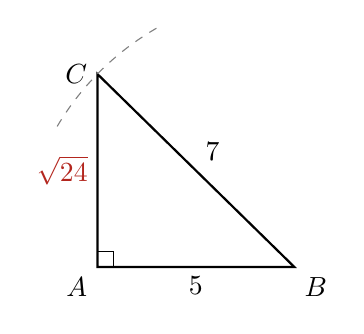
\begin{tikzpicture}[scale=0.5]
\draw[thick] (0,0) node[below left]{$A$} -- (5,0) node[below right]{$B$} -- (0,4.899) node[left]{$C$} -- cycle;
\draw (0,0.4)--(0.4,0.4)--(0.4,0);
\node[below] at (2.5,0){$5$};
\node[above right] at (2.5,2.45){$7$};
\node[left,cThm] at (0,2.45){$\sqrt{24}$};
\draw[dashed,gray] (5,0) ++(120:7) arc (120:150:7);
\end{tikzpicture}\end{LTR}\end{center}

\QQ{2}
\pa $\alpha=1\times5^4+0\times5^3+1\times5^2+4\times5+1=625+25+20+1$: \bx{\alpha=671}.

$\beta=3\times5^3+4\times5^2+0\times5+3=375+100+3$: \bx{\beta=478}.

\pb $b^2-a^2=24$ تعطي حسب 1-(ب): $(a;b)=(5;7)$ أو $(1;5)$.
\begin{itemize}
\item $(5;7)$: $671\times5-478\times7=3355-3346=9$ \ok.
\item $(1;5)$: $671-2390=-1719\neq9$ \texttimes.
\end{itemize}
\bx{(a;b)=(5;7)}.

\QQ{3}
\pa $2013=1434\times1+579$ ، $1434=579\times2+276$ ، $579=276\times2+27$ ، $276=27\times10+6$ ، $27=6\times4+3$ ، $6=3\times2+0$.
إذن \bx{\pgcd(2013;1434)=3}.

$2013=3\times671$ و $1434=3\times478$، إذن $3=\pgcd(2013;1434)=3\,\pgcd(671;478)$، ومنه \bx{\pgcd(671;478)=1}.

\pb بالقسمة على $3$: $2013x-1434y=27\iff671x-478y=9$. حسب 2-(ب): $(5;7)$ حل خاص.

$671x-478y=671\times5-478\times7\iff671(x-5)=478(y-7)$.

$\pgcd(671;478)=1$ و $478\mid671(x-5)$، فحسب غوص $478\mid x-5$: $x=478k+5$، ثم $y=671k+7$.

\bxt{$S=\left\{(478k+5\,;\,671k+7)\ /\ k\in\Z\right\}$}.
\end{hal}

% ===================== 2012 م1 =====================
\begin{tamrin}{بكالوريا 2012 -- الموضوع الأول -- شعبة رياضيات}
نعتبر في $\Z^2$ المعادلة ذات المجهول $(x;y)$ التالية: $2011x-1432y=31\ \ldots(1)$.

\textbf{1.}
\begin{sq}
\qa بيّن أن العدد $2011$ أولي.
\qb باستعمال خوارزمية إقليدس، عيّن حلًّا خاصًا $(x_0;y_0)$ للمعادلة $(1)$، ثم حل المعادلة $(1)$.
\end{sq}
\textbf{2.}
\begin{sq}
\qa عيّن تبعًا لقيم العدد الطبيعي $n$، باقي القسمة الإقليدية للعدد $2^n$ على $7$، ثم جد باقي القسمة الإقليدية للعدد $2011^{1432^{2012}}$ على $7$.
\qb عيّن قيم العدد الطبيعي $n$ والتي من أجلها يكون: $2010^n+2011^n+1432^n\equiv0\,[7]$.
\end{sq}
\textbf{3.} $N$ عدد طبيعي يُكتب $\overline{2\gamma\alpha\beta}$ في نظام التعداد ذي الأساس $9$ حيث: $\alpha$ ، $\beta$ و $\gamma$ بهذا الترتيب تشكل حدودًا متتابعة من متتالية حسابية متزايدة تماما، و $(\beta;\gamma)$ حل للمعادلة $(1)$.
عيّن $\alpha$ ، $\beta$ و $\gamma$ ثم اكتب $N$ في النظام العشري.
\end{tamrin}

\begin{hal}
\QQ{1}
\pa $\sqrt{2011}\approx44{,}8$. نتحقق أن $2011$ لا يقبل القسمة على أي عدد أولي $p\le43$:
\begin{itemize}
\item $2011$ فردي؛ مجموع أرقامه $4$ فلا يقبل القسمة على $3$؛ لا ينتهي بـ $0$ أو $5$.
\item $2011=7\times287+2$ ، $=11\times182+9$ ، $=13\times154+9$ ، $=17\times118+5$ ، $=19\times105+16$ ، $=23\times87+10$ ، $=29\times69+10$ ، $=31\times64+27$ ، $=37\times54+13$ ، $=41\times49+2$ ، $=43\times46+33$.
\end{itemize}
إذن \bxt{$2011$ عدد أولي}.

\pb خوارزمية إقليدس على $2011$ و $1432$:
\begin{align*}
2011&=1432\times1+579, & 1432&=579\times2+274, & 579&=274\times2+31.
\end{align*}
نلاحظ ظهور الباقي $31$، فنعبّر عنه بدلالة $2011$ و $1432$:
\begin{align*}
579&=2011-1432,\\
274&=1432-2\times579=1432-2(2011-1432)=3\times1432-2\times2011,\\
31&=579-2\times274=(2011-1432)-2(3\times1432-2\times2011)=5\times2011-7\times1432.
\end{align*}
إذن $2011\times5-1432\times7=31$: \bx{(x_0;y_0)=(5;7)}.

\textbf{الحل العام:} $2011x-1432y=2011\times5-1432\times7\iff2011(x-5)=1432(y-7)$.

$2011$ أولي ولا يقسم $1432$ (لأن $1432<2011$)، إذن $\pgcd(2011;1432)=1$. وحسب غوص: $1432\mid x-5$، أي $x=1432k+5$، ثم $y=2011k+7$.

\bxt{$S=\left\{(1432k+5\,;\,2011k+7)\ /\ k\in\Z\right\}$}.

\QQ{2}
\pa $2^3\equiv1\,[7]$، والبواقي دورية ودورها $3$:
\begin{center}
\begin{tabular}{|c|c|c|c|}\hline
$n$ & $3k$ & $3k+1$ & $3k+2$\\\hline
$2^n\equiv\ldots\,[7]$ & $1$ & $2$ & $4$\\\hline
\end{tabular}
\end{center}
$2011=7\times287+2$، أي $2011\equiv2\,[7]$، إذن $2011^{1432^{2012}}\equiv2^{1432^{2012}}\,[7]$، ويكفي معرفة باقي الأس $1432^{2012}$ على $3$:
$1432=3\times477+1$، أي $1432\equiv1\,[3]$، ومنه $1432^{2012}\equiv1\,[3]$، أي الأس من الشكل $3k+1$.

إذن $2011^{1432^{2012}}\equiv2\,[7]$: \bxt{الباقي هو $2$}.

\pb $2010\equiv1\,[7]$ ، $2011\equiv2\,[7]$ ، $1432=7\times204+4\equiv4=2^2\,[7]$. إذن:
\[2010^n+2011^n+1432^n\equiv1+2^n+2^{2n}\,[7].\]
\begin{center}
\begin{tabular}{|c|c|c|c|}\hline
$n$ & $3k$ & $3k+1$ & $3k+2$\\\hline
$2^n\equiv$ & $1$ & $2$ & $4$\\\hline
$2^{2n}\equiv$ & $1$ & $4$ & $2$\\\hline
$1+2^n+2^{2n}\equiv$ & $3$ & $0$ & $0$\\\hline
\end{tabular}
\end{center}
(مثلا $n=3k+2$: $2n=6k+4=3(2k+1)+1$، فـ $2^{2n}\equiv2$، و $1+4+2=7\equiv0$.)

\bxt{$2010^n+2011^n+1432^n\equiv0\,[7]$ $\iff$ $n$ ليس مضاعفًا لـ $3$ ($n=3k+1$ أو $n=3k+2$)}.

\QQ{3} الأرقام في الأساس $9$: $0\le\alpha,\beta,\gamma\le8$.

$(\beta;\gamma)$ حل لـ $(1)$: $\beta=1432k+5$ و $\gamma=2011k+7$. من $0\le\beta\le8$ نجد $k=0$، إذن $\beta=5$ و $\gamma=7$.

$\alpha$ ، $\beta$ ، $\gamma$ حدود متتابعة لمتتالية حسابية: $2\beta=\alpha+\gamma$، ومنه $\alpha=10-7=3$. والمتتالية متزايدة تماما ($3<5<7$، أساسها $2$) \ok.

\bx{\alpha=3}\ ،\ \bx{\beta=5}\ ،\ \bx{\gamma=7}، و $N=\overline{2735}$ في الأساس $9$:
\[N=2\times9^3+7\times9^2+3\times9+5=1458+567+27+5,\]
أي \bx{N=2057}.
\end{hal}

% ===================== 2012 م2 =====================
\begin{tamrin}{بكالوريا 2012 -- الموضوع الثاني -- شعبة رياضيات}
$(u_n)$ هي المتتالية العددية المعرفة على $\N$ كما يلي: $u_0=16$، ومن أجل كل عدد طبيعي $n$: $u_{n+1}=6u_n-9$.

\textbf{1.}
\begin{sq}
\qa أحسب بواقي قسمة كل من الحدود $u_0$ ، $u_1$ ، $u_2$ ، $u_3$ و $u_4$ على $7$.
\qb خمّن قيمة العدد $a$ وقيمة العدد $b$ بحيث: $u_{2k}\equiv a\,[7]$ و $u_{2k+1}\equiv b\,[7]$.
\end{sq}
\textbf{2.}
\begin{sq}
\qa برهن أنه، من أجل كل عدد طبيعي $n$: $u_{n+2}\equiv u_n\,[7]$.
\qb برهن بالتراجع أنه من أجل كل عدد طبيعي $k$: $u_{2k}\equiv2\,[7]$، ثم استنتج أن: $u_{2k+1}\equiv3\,[7]$.
\end{sq}
\textbf{3.} نضع من أجل كل عدد طبيعي $n$: $v_n=u_n-\dfrac95$.
\begin{sq}
\qa بيّن أن المتتالية $(v_n)$ هندسية، يُطلب تعيين أساسها وحدها الأول.
\qb أحسب بدلالة $n$ كلًّا من $u_n$ و $S_n$ حيث: $S_n=u_0+u_1+\cdots+u_n$.
\end{sq}
\textbf{4.} $n$ عدد طبيعي غير معدوم.
\begin{sq}
\qa أحسب بدلالة $n$ المجموع $S$ بحيث: $S=u_0+u_1+u_2+\cdots+u_{2n}$.
\qb استنتج بدلالة $n$ المجموعين $S_1$ و $S_2$ حيث: $S_1=u_0+u_2+u_4+\cdots+u_{2n}$ و $S_2=u_1+u_3+u_5+\cdots+u_{2n-1}$.
\end{sq}
\end{tamrin}

\begin{hal}
\QQ{1}
\pa نعمل بترديد $7$: $6\equiv-1$ و $-9\equiv-2\,[7]$، إذن $u_{n+1}\equiv-u_n-2\,[7]$.
\begin{itemize}
\item $u_0=16=7\times2+2$: $u_0\equiv2\,[7]$.
\item $u_1=6\times16-9=87=7\times12+3$: $u_1\equiv3\,[7]$.
\item $u_2=6\times87-9=513=7\times73+2$: $u_2\equiv2\,[7]$.
\item $u_3\equiv-2-2=-4\equiv3\,[7]$ ($u_3=3069$).
\item $u_4\equiv-3-2=-5\equiv2\,[7]$ ($u_4=18405$).
\end{itemize}
\begin{center}
\begin{tabular}{|c|c|c|c|c|c|}\hline
$n$ & $0$ & $1$ & $2$ & $3$ & $4$\\\hline
$u_n\equiv\ldots\,[7]$ & $2$ & $3$ & $2$ & $3$ & $2$\\\hline
\end{tabular}
\end{center}

\pb نخمّن: \bx{a=2}\ و\ \bx{b=3}.

\QQ{2}
\pa $u_{n+2}=6u_{n+1}-9=6(6u_n-9)-9=36u_n-63$.
لكن $36=7\times5+1\equiv1\,[7]$ و $63=7\times9\equiv0\,[7]$، إذن \bx{u_{n+2}\equiv u_n\,[7]}.

\pb $P(k):\ u_{2k}\equiv2\,[7]$.
\begin{itemize}
\item $P(0)$: $u_0=16\equiv2\,[7]$ صحيحة.
\item نفرض $u_{2k}\equiv2\,[7]$. حسب (أ): $u_{2k+2}=u_{2(k+1)}\equiv u_{2k}\equiv2\,[7]$، إذن $P(k+1)$ صحيحة.
\end{itemize}
إذن من أجل كل $k\in\N$: \bx{u_{2k}\equiv2\,[7]}.

\textbf{الاستنتاج:} $u_{2k+1}=6u_{2k}-9\equiv6\times2-9=3\,[7]$، أي \bx{u_{2k+1}\equiv3\,[7]}.

\QQ{3}
\pa $v_{n+1}=u_{n+1}-\dfrac95=6u_n-9-\dfrac95=6u_n-\dfrac{54}{5}=6\left(u_n-\dfrac95\right)=6v_n$.

\bxt{$(v_n)$ هندسية أساسها $q=6$ وحدها الأول $v_0=16-\frac95=\frac{71}{5}$}.

\pb $v_n=\dfrac{71}{5}\times6^n$، ومنه \bx{u_n=\dfrac{71}{5}\times6^n+\dfrac95}.

$S_n=\displaystyle\sum_{k=0}^{n}\left(v_k+\frac95\right)=v_0\times\frac{6^{n+1}-1}{6-1}+\frac95(n+1)=\frac{71}{25}\left(6^{n+1}-1\right)+\frac{9(n+1)}{5}$.

\bx{S_n=\dfrac{71\left(6^{n+1}-1\right)+45(n+1)}{25}}.

تحقق: $S_1=\dfrac{71\times35+90}{25}=\dfrac{2575}{25}=103=16+87$ \ok.

\QQ{4}
\pa $S=S_{2n}$ (المجموع من $u_0$ إلى $u_{2n}$)، إذن بتعويض $n$ بـ $2n$:
\bx{S=\dfrac{71\left(6^{2n+1}-1\right)+45(2n+1)}{25}}.

\pb \textbf{حساب $S_1$:} $S_1=\displaystyle\sum_{k=0}^{n}u_{2k}=\sum_{k=0}^{n}\left(\frac{71}{5}\times36^k+\frac95\right)$. الحدود $\frac{71}{5}\times36^k$ تشكل متتالية هندسية أساسها $36$، وعددها $n+1$:
\[S_1=\frac{71}{5}\times\frac{36^{n+1}-1}{35}+\frac{9(n+1)}{5}=\frac{71\left(36^{n+1}-1\right)}{175}+\frac{9(n+1)}{5}.\]
\bx{S_1=\dfrac{71\left(36^{n+1}-1\right)+315(n+1)}{175}}.

\textbf{حساب $S_2$:} $S=S_1+S_2$، إذن $S_2=S-S_1$. أو مباشرة: $S_2=\displaystyle\sum_{k=0}^{n-1}u_{2k+1}=\sum_{k=0}^{n-1}\left(\frac{426}{5}\times36^k+\frac95\right)$ (لأن $\frac{71}{5}\times6^{2k+1}=\frac{426}{5}\times36^k$):
\[S_2=\frac{426}{5}\times\frac{36^n-1}{35}+\frac{9n}{5}.\]
\bx{S_2=\dfrac{426\left(36^n-1\right)+315n}{175}}.

تحقق ($n=1$): $S_1=\dfrac{71\times1295+630}{175}=529=16+513$ \ok، و $S_2=\dfrac{426\times35+315}{175}=87=u_1$ \ok.
\end{hal}

% ===================== 2011 م1 =====================
\begin{tamrin}{بكالوريا 2011 -- الموضوع الأول -- شعبة رياضيات}
$(u_n)$ متتالية حسابية متزايدة تماما حدودها أعداد طبيعية تحقق: $\begin{cases}u_4=15\\ m+d=42\end{cases}$ حيث $\begin{cases}m=\ppcm(u_3;u_5)\\ d=\pgcd(u_3;u_5)\end{cases}$

\textbf{1.} عيّن الحدين $u_3$ و $u_5$ ثم استنتج $u_0$.

\textbf{2.} اكتب $u_n$ بدلالة $n$، ثم بيّن أن $2010$ حد من حدود المتتالية $(u_n)$ وعيّن رتبته.

\textbf{3.} عيّن الحد الذي ابتداءً منه يكون مجموع $5$ حدود متعاقبة من $(u_n)$ يساوي $10080$.

\textbf{4.} $n$ عدد طبيعي غير معدوم.
\begin{sq}
\qa أحسب بدلالة $n$ المجموع $S$ بحيث: $S=u_0+u_1+u_2+\cdots+u_{2n}$.
\qb استنتج بدلالة $n$ المجموعين $S_1$ و $S_2$ حيث: $S_1=u_0+u_2+u_4+\cdots+u_{2n}$ و $S_2=u_1+u_3+u_5+\cdots+u_{2n-1}$.
\end{sq}
\end{tamrin}

\begin{hal}
\QQ{1} ليكن $r$ أساس المتتالية. الحدود طبيعية، إذن $r=u_5-u_4$ عدد صحيح، و $r>0$ (متزايدة تماما)، أي $r\in\N^*$.

$u_3=15-r$ و $u_5=15+r$، إذن $u_3+u_5=30$.

$d$ يقسم $u_3$ و $u_5$ فهو يقسم مجموعهما $30$، و $d$ يقسم $m$ فهو يقسم $m+d=42$. إذن $d$ يقسم $\pgcd(30;42)=6$: $d\in\{1;2;3;6\}$.

نضع $u_3=da'$ و $u_5=db'$ مع $\pgcd(a';b')=1$ و $a'<b'$. إذن $m=da'b'$، و:
\[\begin{cases}d(a'+b')=30\\ d(1+a'b')=42\end{cases}\iff\begin{cases}a'+b'=\frac{30}{d}\\ a'b'=\frac{42}{d}-1\end{cases}\]
\begin{center}
\begin{tabular}{|c|c|c|c|c|}\hline
$d$ & $1$ & $2$ & $3$ & $6$\\\hline
$a'+b'$ & $30$ & $15$ & $10$ & $5$\\\hline
$a'b'$ & $41$ & $20$ & $13$ & $6$\\\hline
\end{tabular}
\end{center}
\begin{itemize}
\item $d=1$: $a'b'=41$ (أولي) يعطي $\{1;41\}$ ومجموعهما $42\neq30$: مرفوض.
\item $d=2$: $a'b'=20$: الثنائيات الأولية فيما بينها $\{1;20\}$ و $\{4;5\}$ ومجموعهما $21$ و $9$، لا يساوي $15$: مرفوض.
\item $d=3$: $a'b'=13$: $\{1;13\}$ مجموعهما $14\neq10$: مرفوض.
\item $d=6$: $a'b'=6$ و $a'+b'=5$: $a'=2$ ، $b'=3$ (أوليان فيما بينهما) \ok.
\end{itemize}
إذن \bx{u_3=12}\ و\ \bx{u_5=18}، و $r=3$. تحقق: $\pgcd(12;18)=6$ ، $\ppcm(12;18)=36$ ، $36+6=42$ \ok.

$u_0=u_3-3r=12-9$، أي \bx{u_0=3}.

\QQ{2} $u_n=u_0+nr$، أي \bx{u_n=3n+3}.

$u_n=2010\iff3n+3=2010\iff n=669\in\N$. إذن $2010$ حد من حدود المتتالية وهو \bx{u_{669}}، ورتبته \bx{670} (لأن الحد الأول هو $u_0$).

\QQ{3} ليكن $u_p$ أول هذه الحدود الخمسة: $u_p+u_{p+1}+\cdots+u_{p+4}=\dfrac{5\left(u_p+u_{p+4}\right)}{2}=\dfrac{5\left(3p+3+3p+15\right)}{2}=15p+45$.
\[15p+45=10080\iff15p=10035\iff p=669.\]
\bxt{الحد المطلوب هو $u_{669}=2010$} (والحدود هي $2010$ ، $2013$ ، $2016$ ، $2019$ ، $2022$ ومجموعها $10080$ \ok).

\QQ{4}
\pa $S$ مجموع $2n+1$ حدًّا متتابعًا:
$S=\dfrac{(2n+1)\left(u_0+u_{2n}\right)}{2}=\dfrac{(2n+1)(3+6n+3)}{2}$، أي \bx{S=3(2n+1)(n+1)}.

\pb $u_{2k}=6k+3$: الحدود $u_0,u_2,\ldots,u_{2n}$ تشكل متتالية حسابية أساسها $6$، عددها $n+1$:
$S_1=\dfrac{(n+1)(u_0+u_{2n})}{2}=\dfrac{(n+1)(6n+6)}{2}$، أي \bx{S_1=3(n+1)^2}.

$S=S_1+S_2$، إذن $S_2=3(n+1)(2n+1)-3(n+1)^2=3(n+1)(2n+1-n-1)$، أي \bx{S_2=3n(n+1)}.

تحقق ($n=1$): $S_1=u_0+u_2=3+9=12=3\times4$ \ok، $S_2=u_1=6=3\times1\times2$ \ok.
\end{hal}

% ===================== 2011 م2 =====================
\begin{tamrin}{بكالوريا 2011 -- الموضوع الثاني -- شعبة رياضيات}
\textbf{1.} نعتبر المعادلة $(E):\ 13x-7y=-1$ حيث $x$ و $y$ عددان صحيحان. حل المعادلة $(E)$.

\textbf{2.} عيّن الأعداد الصحيحة النسبية $a$ بحيث: $\begin{cases}a\equiv-1\,[7]\\ a\equiv0\,[13]\end{cases}$

\textbf{3.} ادرس، حسب قيم العدد الطبيعي $n$، بواقي قسمة $9^n$ على كل من $7$ و $13$.

\textbf{4.} ليكن العدد الطبيعي $b$ المكتوب في نظام التعداد ذي الأساس $9$ كما يلي: $b=\overline{\alpha00\beta086}$، حيث $\alpha$ و $\beta$ عددان طبيعيان و $\alpha\neq0$.

عيّن $\alpha$ و $\beta$ حتى يكون $b$ قابلًا للقسمة على $91$.
\end{tamrin}

\begin{hal}
\QQ{1} \textbf{حل خاص:} $(1;2)$ لأن $13\times1-7\times2=-1$.

$13x-7y=13\times1-7\times2\iff13(x-1)=7(y-2)$. بما أن $\pgcd(13;7)=1$ و $7\mid13(x-1)$، فحسب غوص $7\mid x-1$: $x=7k+1$، ثم $13\times7k=7(y-2)$ أي $y=13k+2$.

\bxt{$S=\left\{(7k+1\,;\,13k+2)\ /\ k\in\Z\right\}$}.

\QQ{2} $a\equiv0\,[13]\iff a=13x$ ، و $a\equiv-1\,[7]\iff a=7y-1$ ($x,y\in\Z$).

إذن $13x=7y-1$، أي $13x-7y=-1$: $(x;y)$ حل لـ $(E)$، ومنه $x=7k+1$ و $a=13(7k+1)=91k+13$.

\bxt{$a=91k+13$ مع $k\in\Z$، أي $a\equiv13\,[91]$}.

\QQ{3} \textbf{بترديد 7:} $9\equiv2\,[7]$: $9^0\equiv1$ ، $9^1\equiv2$ ، $9^2\equiv4$ ، $9^3\equiv8\equiv1\,[7]$.

\textbf{بترديد 13:} $9^0\equiv1$ ، $9^1\equiv9$ ، $9^2=81=13\times6+3\equiv3$ ، $9^3\equiv27\equiv1\,[13]$.

في الحالتين $9^3\equiv1$، فالبواقي دورية ودورها $3$:
\begin{center}
\begin{tabular}{|c|c|c|c|}\hline
$n$ & $3k$ & $3k+1$ & $3k+2$\\\hline
$9^n\equiv\ldots\,[7]$ & $1$ & $2$ & $4$\\\hline
$9^n\equiv\ldots\,[13]$ & $1$ & $9$ & $3$\\\hline
\end{tabular}
\end{center}

\QQ{4} الأرقام في الأساس $9$: $1\le\alpha\le8$ و $0\le\beta\le8$.
\[b=\alpha\times9^6+0\times9^5+0\times9^4+\beta\times9^3+0\times9^2+8\times9+6=\alpha\times9^6+\beta\times9^3+78.\]
$6$ و $3$ مضاعفان لـ $3$، إذن $9^6\equiv9^3\equiv1$ بترديد $7$ وبترديد $13$:
\begin{itemize}
\item $b\equiv\alpha+\beta+78\equiv\alpha+\beta+1\,[7]$ (لأن $78=7\times11+1$).
\item $b\equiv\alpha+\beta+78\equiv\alpha+\beta\,[13]$ (لأن $78=13\times6$).
\end{itemize}
$91=7\times13$ و $\pgcd(7;13)=1$، إذن $91\mid b\iff7\mid b$ و $13\mid b$:
\[\begin{cases}\alpha+\beta\equiv-1\,[7]\\ \alpha+\beta\equiv0\,[13]\end{cases}\]
حسب السؤال 2: $\alpha+\beta\equiv13\,[91]$. لكن $1\le\alpha+\beta\le16$، إذن $\alpha+\beta=13$.

مع $\alpha\le8$ و $\beta\le8$: $\alpha\ge5$.

\bxt{$(\alpha;\beta)\in\{(5;8)\,;\,(6;7)\,;\,(7;6)\,;\,(8;5)\}$}.

تحقق: $\overline{5008086}_{(9)}=5\times531441+8\times729+78=2663115=91\times29265$ \ok.
\end{hal}

% ===================== 2010 م1 =====================
\begin{tamrin}{بكالوريا 2010 -- الموضوع الأول -- شعبة رياضيات}
\textbf{1.} نعتبر في $\Z^2$ المعادلة: $7x+65y=2009\ \ldots(1)$.
\begin{sq}
\qa بيّن أنه إذا كانت الثنائية $(x;y)$ حلًّا للمعادلة $(1)$ فإن $y$ مضاعف للعدد $7$.
\qb حل المعادلة $(1)$.
\end{sq}
\textbf{2.} ادرس، حسب قيم العدد الطبيعي $n$، بواقي القسمة الإقليدية للعدد $2^n$ على $9$.

\textbf{3.} عيّن قيم العدد الطبيعي $n$، بحيث يقبل العدد $2^{6n}+3n+2$ القسمة على $9$.

\textbf{4.} نضع من أجل كل عدد طبيعي $n$: $u_n=2^{6n}-1$.
\begin{sq}
\qa تحقق أن $u_n$ يقبل القسمة على $9$.
\qb حل المعادلة $(2):\ (7u_1)x+(u_2)y=126567$ ذات المجهول $(x;y)$ حيث $x$ و $y$ عددان صحيحان.
\qc عيّن الثنائية $(x_0;y_0)$ حل المعادلة $(2)$ حيث $x_0$ و $y_0$ عددان طبيعيان مع $y_0\ge25$.
\end{sq}
\end{tamrin}

\begin{hal}
\QQ{1}
\pa $2009=7\times287$. إذا كان $(x;y)$ حلًّا: $65y=2009-7x=7(287-x)$، إذن $7\mid65y$. و $\pgcd(7;65)=1$ ($65=5\times13$)، فحسب غوص: \bxt{$7$ يقسم $y$}.

\pb نضع $y=7k$ ($k\in\Z$): $7x+455k=2009\iff x+65k=287\iff x=287-65k$.

وعكسيًا: $7(287-65k)+65\times7k=2009$ \ok.

\bxt{$S=\left\{(287-65k\,;\,7k)\ /\ k\in\Z\right\}$}.

\QQ{2} $2^0\equiv1$ ، $2^1\equiv2$ ، $2^2\equiv4$ ، $2^3\equiv8$ ، $2^4=16\equiv7$ ، $2^5\equiv14\equiv5$ ، $2^6\equiv10\equiv1\,[9]$. الدور $6$:
\begin{center}
\begin{tabular}{|c|c|c|c|c|c|c|}\hline
$n$ & $6k$ & $6k+1$ & $6k+2$ & $6k+3$ & $6k+4$ & $6k+5$\\\hline
$2^n\equiv\ldots\,[9]$ & $1$ & $2$ & $4$ & $8$ & $7$ & $5$\\\hline
\end{tabular}
\end{center}

\QQ{3} $2^{6n}\equiv1\,[9]$، إذن $2^{6n}+3n+2\equiv3n+3=3(n+1)\,[9]$.
\[9\mid3(n+1)\iff3\mid n+1\iff n\equiv2\,[3].\]
\bxt{$n=3k+2$ مع $k\in\N$}.

\QQ{4}
\pa $2^{6n}\equiv1\,[9]$، إذن $u_n=2^{6n}-1\equiv0\,[9]$: \bxt{$u_n$ يقبل القسمة على $9$}.

\pb $u_1=2^6-1=63$ ، $7u_1=441=3^2\times7^2$ ، $u_2=2^{12}-1=4095=3^2\times5\times7\times13$.

$\pgcd(441;4095)=3^2\times7=63$، و $126567=63\times2009$. بقسمة الطرفين على $63$:
\[(2):\ 441x+4095y=126567\iff7x+65y=2009\iff(1).\]
\bxt{حلول $(2)$: $(x;y)=(287-65k\,;\,7k)$ مع $k\in\Z$}.

\pc $y_0=7k\ge25\iff k\ge\frac{25}{7}\approx3{,}57$، أي $k\ge4$. و $x_0=287-65k\ge0\iff k\le\frac{287}{65}\approx4{,}4$، أي $k\le4$.

إذن $k=4$: \bx{(x_0;y_0)=(27;28)}. تحقق: $441\times27+4095\times28=11907+114660=126567$ \ok.
\end{hal}

% ===================== 2010 م2 =====================
\begin{tamrin}{بكالوريا 2010 -- الموضوع الثاني -- شعبة رياضيات}
\textbf{1.} برهن أنه من أجل كل عدد طبيعي $n$، العدد $3^{3n}-1$ يقبل القسمة على $13$.

\textbf{2.} استنتج أنه من أجل كل عدد طبيعي $n$، يقبل كل من العددين $3^{3n+1}-3$ و $3^{3n+2}-9$ القسمة على $13$.

\textbf{3.} عيّن، حسب قيم $n$، باقي القسمة الإقليدية للعدد $3^n$ على $13$، واستنتج باقي قسمة $2005^{2010}$ على $13$.

\textbf{4.} نضع من أجل كل عدد طبيعي $p$: $A_p=3^p+3^{2p}+3^{3p}$.
\begin{sq}
\qa من أجل $p=3n$، عيّن باقي القسمة الإقليدية للعدد $A_p$ على $13$.
\qb برهن أنه من أجل $p=3n+1$، فإن $A_p$ يقبل القسمة على $13$.
\qc عيّن باقي القسمة الإقليدية لـ $A_p$ على $13$ من أجل $p=3n+2$.
\end{sq}
\textbf{5.} يُكتب العددان $a$ و $b$ في نظام العد ذي الأساس $3$ كما يلي: $a=\overline{1001001000}$ و $b=\overline{1000100010000}$.
\begin{sq}
\qa تحقق أن $a$ و $b$ يُكتبان على الشكل $A_p$ في النظام العشري.
\qb استنتج باقي القسمة الإقليدية لكل من $a$ و $b$ على $13$.
\end{sq}
\end{tamrin}

\begin{hal}
\QQ{1} $3^{3n}=\left(3^3\right)^n=27^n$ و $27=2\times13+1\equiv1\,[13]$، إذن $27^n\equiv1\,[13]$، ومنه $3^{3n}-1\equiv0\,[13]$: \bxt{$13$ يقسم $3^{3n}-1$}.

\QQ{2} $3^{3n+1}-3=3\left(3^{3n}-1\right)$ و $3^{3n+2}-9=9\left(3^{3n}-1\right)$، وكلاهما مضاعف لـ $3^{3n}-1$ الذي يقبل القسمة على $13$. \bxt{إذن كلاهما يقبل القسمة على $13$}.

\QQ{3} من 1 و 2: $3^{3n}\equiv1$ ، $3^{3n+1}\equiv3$ ، $3^{3n+2}\equiv9\,[13]$:
\begin{center}
\begin{tabular}{|c|c|c|c|}\hline
$n$ & $3k$ & $3k+1$ & $3k+2$\\\hline
$3^n\equiv\ldots\,[13]$ & $1$ & $3$ & $9$\\\hline
\end{tabular}
\end{center}
$2005=13\times154+3$، أي $2005\equiv3\,[13]$، و $2010=3\times670$، إذن $2005^{2010}\equiv3^{3\times670}\equiv1\,[13]$: \bxt{الباقي هو $1$}.

\QQ{4}
\pa $p=3n$: $2p=6n=3(2n)$ و $3p=9n=3(3n)$، إذن $A_p\equiv1+1+1=3\,[13]$: \bxt{الباقي هو $3$}.

\pb $p=3n+1$: $2p=6n+2=3(2n)+2$ و $3p=9n+3=3(3n+1)$، إذن $A_p\equiv3+9+1=13\equiv0\,[13]$: \bxt{$A_p$ يقبل القسمة على $13$}.

\pc $p=3n+2$: $2p=6n+4=3(2n+1)+1$ و $3p=9n+6=3(3n+2)$، إذن $A_p\equiv9+3+1=13\equiv0\,[13]$: \bxt{الباقي هو $0$}.

\QQ{5}
\pa في $a=\overline{1001001000}_{(3)}$ (عشرة أرقام)، الأرقام $1$ في المراتب $9$ ، $6$ ، $3$:
\[a=3^9+3^6+3^3=3^3+3^{2\times3}+3^{3\times3}=A_3.\]
في $b=\overline{1000100010000}_{(3)}$ (ثلاثة عشر رقمًا)، الأرقام $1$ في المراتب $12$ ، $8$ ، $4$:
\[b=3^{12}+3^8+3^4=3^4+3^{2\times4}+3^{3\times4}=A_4.\]
\bx{a=A_3=20439}\ و\ \bx{b=A_4=538083}.

\pb $3=3\times1$ من الشكل $3n$: $a\equiv3\,[13]$. و $4=3\times1+1$ من الشكل $3n+1$: $b\equiv0\,[13]$.

\bxt{باقي $a$ على $13$ هو $3$، وباقي $b$ على $13$ هو $0$}.
\end{hal}

% ===================== 2009 م1 =====================
\begin{tamrin}{بكالوريا 2009 -- الموضوع الأول -- شعبة رياضيات}
$x$ عدد طبيعي أكبر تماما من $1$ و $y$ عدد طبيعي. $A$ عدد طبيعي يُكتب في النظام ذي الأساس $x$ بالشكل: $A=\overline{5566}$.

\textbf{1.}
\begin{sq}
\qa انشر العبارة $\left(5x^2+6\right)(x+1)$، ثم جد علاقة تربط بين $x$ و $y$ إذا علمت أن: $A=\left(5x^2+6\right)(2+2y)$.
\qb أحسب $x$ و $y$ إذا علمت أن $x$ عدد أولي أصغر من $12$، ثم اكتب تبعًا لذلك العدد $A$ في نظام التعداد العشري.
\end{sq}
\textbf{2.}
\begin{sq}
\qa عيّن الأعداد الطبيعية التي مربعاتها تقسم العدد $584$.
\qb عيّن الأعداد الطبيعية $a$ و $b$ حيث $a>b$ التي تحقق: $\begin{cases}a+b=32\\ a^2+b^2=584\end{cases}$
\end{sq}
\end{tamrin}

\begin{hal}
\QQ{1}
\pa $\left(5x^2+6\right)(x+1)=5x^3+5x^2+6x+6$.

من جهة أخرى، في الأساس $x$ (والأرقام $5$ و $6$ تفرض $x\ge7$): $A=5x^3+5x^2+6x+6$. إذن $A=\left(5x^2+6\right)(x+1)$.
\[A=\left(5x^2+6\right)(2+2y)\iff\left(5x^2+6\right)(x+1)=\left(5x^2+6\right)\times2(y+1).\]
وبما أن $5x^2+6\neq0$: $x+1=2y+2$، أي \bx{x=2y+1}.

\pb $x$ أولي، $x<12$ و $x\ge7$: $x\in\{7;11\}$ (وكلاهما فردي يحقق $x=2y+1$).
\begin{itemize}
\item $x=7$: $y=3$ ، و $A=(5\times49+6)(7+1)=251\times8=2008$.
\item $x=11$: $y=5$ ، و $A=(5\times121+6)(11+1)=611\times12=7332$.
\end{itemize}
\bxt{$(x;y)=(7;3)$ و $A=2008$، أو $(x;y)=(11;5)$ و $A=7332$}.

\QQ{2}
\pa $584=2^3\times73$. إذا كان $k^2\mid584$ فإن كل عامل أولي لـ $k$ يظهر في $584$ بأس $\ge2$؛ العامل $73$ أسه $1$ فلا يظهر في $k$، و $2^2\mid2^3$ لكن $2^4\nmid2^3$. إذن $k=1$ أو $k=2$.

\bxt{الأعداد هي: $1$ و $2$}.

\pb ليكن $\delta=\pgcd(a;b)$: $\delta^2$ يقسم $a^2+b^2=584$، فحسب (أ) $\delta\in\{1;2\}$.
\begin{itemize}
\item إذا $\delta=1$: $a+b=32$ زوجي، و $a$ ، $b$ أوليان فيما بينهما فلا يمكن أن يكونا زوجيين معًا، إذن كلاهما فردي، ومنه $a^2+b^2\equiv1+1=2\,[4]$، لكن $584\equiv0\,[4]$: تناقض.
\item إذن $\delta=2$: $a=2a'$ ، $b=2b'$ مع $a'+b'=16$ و $a'^2+b'^2=146$.
\end{itemize}
$a'b'=\dfrac{(a'+b')^2-\left(a'^2+b'^2\right)}{2}=\dfrac{256-146}{2}=55$. إذن $a'$ و $b'$ حلّا $X^2-16X+55=0$، أي $(X-5)(X-11)=0$.

بما أن $a>b$: $a'=11$ ، $b'=5$، ومنه \bx{a=22}\ و\ \bx{b=10}.

تحقق: $22+10=32$ و $484+100=584$ \ok.
\end{hal}

% ===================== 2008 م1 =====================
\begin{tamrin}{بكالوريا 2008 -- الموضوع الأول -- شعبة رياضيات}
نعتبر المعادلة $(E)$ ذات المجهولين الصحيحين $x$ و $y$ حيث: $3x-21y=78$.

\textbf{1.}
\begin{sq}
\qa بيّن أن المعادلة $(E)$ تقبل حلولًا في $\Z^2$.
\qb أثبت أنه إذا كانت الثنائية $(x;y)$ من $\Z^2$ حلًّا للمعادلة $(E)$ فإن $x\equiv5\,[7]$. استنتج حلول المعادلة $(E)$.
\end{sq}
\textbf{2.}
\begin{sq}
\qa ادرس، حسب قيم العدد الطبيعي $n$، بواقي القسمة الإقليدية للعدد $5^n$ على $7$.
\qb عيّن الثنائيات $(x;y)$ من $\N^2$ التي هي حلول المعادلة $(E)$ وتحقق: $5^x+5^y\equiv3\,[7]$.
\end{sq}
\end{tamrin}

\begin{hal}
\QQ{1}
\pa $\pgcd(3;21)=3$ و $78=3\times26$، أي $\pgcd(3;21)$ يقسم $78$: \bxt{$(E)$ تقبل حلولًا في $\Z^2$}.

\pb بالقسمة على $3$: $(E)\iff x-7y=26\iff x=26+7y$. إذن $x\equiv26\,[7]$، و $26=7\times3+5$، ومنه \bx{x\equiv5\,[7]}.

\textbf{الحلول:} $x=7k+5$ ($k\in\Z$)، ثم $7y=x-26=7k-21$، أي $y=k-3$.

\bxt{$S=\left\{(7k+5\,;\,k-3)\ /\ k\in\Z\right\}$}.

\QQ{2}
\pa $5^0\equiv1$ ، $5^1\equiv5$ ، $5^2=25\equiv4$ ، $5^3\equiv20\equiv6$ ، $5^4\equiv30\equiv2$ ، $5^5\equiv10\equiv3$ ، $5^6\equiv15\equiv1\,[7]$. الدور $6$:
\begin{center}
\begin{tabular}{|c|c|c|c|c|c|c|}\hline
$n$ & $6k$ & $6k+1$ & $6k+2$ & $6k+3$ & $6k+4$ & $6k+5$\\\hline
$5^n\equiv\ldots\,[7]$ & $1$ & $5$ & $4$ & $6$ & $2$ & $3$\\\hline
\end{tabular}
\end{center}

\pb الحلول في $\N^2$: $y=k-3\ge0$، نضع $y=m\in\N$، فيكون $x=7m+26$ (طبيعي).

$x=7m+26=6(m+4)+(m+2)$، أي $x\equiv m+2\,[6]$، ومنه $5^x\equiv5^{m+2}\,[7]$ (لأن $5^6\equiv1$). إذن:
\[5^x+5^y\equiv5^{m+2}+5^m=5^m\left(25+1\right)=26\times5^m\equiv5\times5^m=5^{m+1}\,[7].\]
\[5^x+5^y\equiv3\,[7]\iff5^{m+1}\equiv3\,[7]\iff m+1\equiv5\,[6]\iff m\equiv4\,[6].\]
(من الجدول: الباقي $3$ يقابل فقط الأسس من الشكل $6k+5$.)

$m=6p+4$: $y=6p+4$ و $x=7(6p+4)+26=42p+54$.

\bxt{$(x;y)=(42p+54\,;\,6p+4)$ مع $p\in\N$}.

تحقق ($p=0$): $3\times54-21\times4=162-84=78$ \ok، و $5^{54}+5^4\equiv1+2=3\,[7]$ \ok.
\end{hal}

\section{تمارين البكالوريا -- شعبة تقني رياضي}
% ================= التمرين: بكالوريا 2026 م1 =================
\begin{tamrin}{بكالوريا 2026 -- الموضوع الأول -- تقني رياضي}
\QQ{1} نعتبر المعادلة $(E)$: \ $11x-5y=7$ \ ذات المجهولين الصحيحين $x$ و$y$.
\begin{sq}
\qa بيّن أنه إذا كانت الثنائية $(x;y)$ حلًّا للمعادلة $(E)$ فإن $y\equiv 3\ [11]$، ثم حل المعادلة $(E)$.
\qb عيّن الثنائيات $(x;y)$ حلول المعادلة $(E)$ التي تحقق: $|y-x|\le 5$.
\end{sq}
\QQ{2} من أجل كل عدد طبيعي $n$، نضع: $a=11n+3$ و$b=5n+2$ و$d=\pgcd(a;b)$.
\begin{sq}
\qa ما هي القيم الممكنة لـ $d$؟
\qb عيّن الثنائيات $(a;b)$ التي من أجلها يكون: $d=7$.
\end{sq}
\QQ{3}
\begin{sq}
\qa ادرس، حسب قيم العدد الطبيعي $n$، بواقي القسمة الإقليدية للعدد $3^n$ على $11$.
\qb استنتج أنه: من أجل كل عدد طبيعي $n$، $a^b\equiv 9\ [11]$.
\qc عيّن قيمة العدد الطبيعي $n$ حتى يكون: $a^{1447}+a^b+a-b-9\equiv 0\ [11]$ و$2015<n<2037$.
\end{sq}
\QQ{4} $\lambda$ عدد طبيعي يُكتب $\overline{5623}$ في نظام التعداد ذي الأساس $7$. اكتب $\lambda$ في نظام التعداد ذي الأساس $6$.
\end{tamrin}

\begin{hal}
\QQ{1}\pa لتكن $(x;y)$ حلًّا للمعادلة $(E)$، إذن $11x-5y=7$، ومنه $5y=11x-7$.

وبما أن $11x\equiv 0\ [11]$ فإن: $5y\equiv -7\ [11]$، أي $5y\equiv 4\ [11]$.

نبحث عن مقلوب $5$ بترديد $11$: لدينا $9\times 5=45=4\times 11+1$، أي $45\equiv 1\ [11]$.

نضرب طرفي الموافقة في $9$: $45y\equiv 36\ [11]$، ومنه $y\equiv 36\ [11]$، و$36=3\times 11+3$، إذن \bx{y\equiv 3\ [11]}.

\textbf{حل المعادلة:} بما أن $y\equiv 3\ [11]$ فإن $y=11k+3$ حيث $k\in\Z$. نعوّض في $(E)$:
\[11x=7+5(11k+3)=55k+22\quad\Longrightarrow\quad x=5k+2.\]
\textbf{التحقق العكسي:} من أجل كل $k\in\Z$: $11(5k+2)-5(11k+3)=55k+22-55k-15=7$ \ok.

إذن مجموعة حلول المعادلة $(E)$ هي: \bx{S=\{(5k+2\,;\,11k+3)\ ;\ k\in\Z\}}

\pb لدينا: $y-x=(11k+3)-(5k+2)=6k+1$. إذن:
\[|y-x|\le 5\iff -5\le 6k+1\le 5\iff -6\le 6k\le 4\iff -1\le k\le \tfrac{2}{3}.\]
وبما أن $k$ عدد صحيح فإن $k\in\{-1;0\}$:
\begin{itemize}
\item من أجل $k=-1$: $(x;y)=(-3;-8)$، و$|y-x|=|-5|=5\le 5$ \ok.
\item من أجل $k=0$: $(x;y)=(2;3)$، و$|y-x|=1\le 5$ \ok.
\end{itemize}
إذن الثنائيات المطلوبة: \bx{(-3;-8)\ ;\ (2;3)}

\QQ{2}\pa $d=\pgcd(a;b)$ يقسم $a$ و$b$، إذن يقسم كل تركيب خطي لهما، وبالخصوص:
\[11b-5a=11(5n+2)-5(11n+3)=55n+22-55n-15=7.\]
إذن $d$ يقسم $7$، و$7$ عدد أولي، ومنه \bx{d\in\{1;7\}}

القيمتان ممكنتان فعلًا: من أجل $n=0$: $a=3$، $b=2$ و$d=1$؛ ومن أجل $n=1$: $a=14$، $b=7$ و$d=7$.

\pb $d=7$ يعني أن $7$ يقسم $a$ و$b$ معًا (لأن $d\in\{1;7\}$).

$7$ يقسم $b$: $5n+2\equiv 0\ [7]$، أي $5n\equiv -2\ [7]$، أي $5n\equiv 5\ [7]$. وبما أن $\pgcd(5;7)=1$ فإن (مبرهنة غوص) $n\equiv 1\ [7]$، أي $n=7k+1$ مع $k\in\N$.

عندئذ:
\begin{itemize}
\item $a=11(7k+1)+3=77k+14=7(11k+2)$ مضاعف لـ $7$ \ok
\item $b=5(7k+1)+2=35k+7=7(5k+1)$ مضاعف لـ $7$ \ok
\end{itemize}

إذن: $d=7\iff n=7k+1$ ($k\in\N$)، والثنائيات المطلوبة: \bx{(a;b)=(77k+14\,;\,35k+7)\ ,\ k\in\N}

\QQ{3}\pa نحسب القوى الأولى للعدد $3$ بترديد $11$:
\[3^0=1,\quad 3^1=3,\quad 3^2=9,\quad 3^3=27\equiv 5,\quad 3^4\equiv 3\times 5=15\equiv 4,\quad 3^5\equiv 3\times 4=12\equiv 1\ [11].\]
بما أن $3^5\equiv 1\ [11]$ فإن البواقي دورية ودورها $5$، لأنه من أجل كل $k\in\N$ و$r\in\{0;1;2;3;4\}$:
\[3^{5k+r}=(3^5)^k\times 3^r\equiv 3^r\ [11].\]
\begin{center}
\begin{tabular}{|C|c|c|c|c|c|}\hline
$n$ & $5k$ & $5k+1$ & $5k+2$ & $5k+3$ & $5k+4$\\\hline
باقي قسمة $3^n$ على $11$ & $1$ & $3$ & $9$ & $5$ & $4$\\\hline
\end{tabular}
\end{center}

\pb $a=11n+3$ إذن $a\equiv 3\ [11]$، ومنه $a^b\equiv 3^b\ [11]$. و$b=5n+2$ من الشكل $5k+2$، إذن حسب الجدول: $3^{5n+2}\equiv 9\ [11]$.
إذن من أجل كل عدد طبيعي $n$: \bx{a^b\equiv 9\ [11]}

\pc لدينا $1447=5\times 289+2$، إذن $a^{1447}\equiv 3^{1447}\equiv 9\ [11]$. ولدينا $a\equiv 3\ [11]$ و$b=5n+2$. إذن:
\[a^{1447}+a^b+a-b-9\equiv 9+9+3-(5n+2)-9\equiv 10-5n\ [11].\]
\[10-5n\equiv 0\ [11]\iff 5n\equiv 10\ [11]\iff n\equiv 2\ [11]\]
(قسمنا على $5$ لأن $\pgcd(5;11)=1$). إذن $n=11k+2$ مع $k\in\N$.

$2015<11k+2<2037\iff 2013<11k<2035\iff 183<k<185$، لأن $\frac{2013}{11}=183$ و$\frac{2035}{11}=185$. إذن $k=184$ و$n=11\times 184+2$: \bx{n=2026}

\QQ{4} نحوّل إلى النظام العشري:
\[\lambda=\overline{5623}^{\,7}=5\times 7^3+6\times 7^2+2\times 7+3=1715+294+14+3=2026.\]
نقسم $2026$ على $6$ قسمات متتالية:
\[2026=6\times 337+4,\quad 337=6\times 56+1,\quad 56=6\times 9+2,\quad 9=6\times 1+3,\quad 1=6\times 0+1.\]
نقرأ البواقي من الأخير إلى الأول: \bx{\lambda=\overline{13214}^{\,6}}

تحقق: $1\times 6^4+3\times 6^3+2\times 6^2+1\times 6+4=1296+648+72+6+4=2026$ \ok.
\end{hal}

% ================= بكالوريا 2026 م2 =================
\begin{tamrin}{بكالوريا 2026 -- الموضوع الثاني -- تقني رياضي}
\QQ{1}
\begin{sq}
\qa عيّن باقي القسمة الإقليدية للعدد $1447$ على $7$، وباقي القسمة الإقليدية للعدد $2687$ على $13$.
\qb برّر أن العدد $1447$ أولي، ثم عيّن القواسم الطبيعية للعدد $2894$.
\qc جد الثنائيات $(x;y)$ من الأعداد الطبيعية التي تحقق: $x(x+y)=2894$.
\end{sq}
\QQ{2} من أجل كل عدد طبيعي $n$، نضع: $a=7n+5$، $b=13n+9$ و$\pgcd(a;b)=d$.

عيّن القيم الممكنة للعدد $d$، ثم حدّد قيم $n$ التي من أجلها يكون $d=2$.

\QQ{3} من أجل كل عدد طبيعي $n$، نضع: $A=14n^2+17n+5$ و$B=26n^2+31n+9$.
\begin{sq}
\qa بيّن أن العدد $(2n+1)$ يقسم كلًّا من $A$ و$B$.
\qb استنتج بدلالة $n$، وحسب قيم $n$، القاسم المشترك الأكبر للعددين $A$ و$B$.
\end{sq}
\QQ{4} من أجل $d=1$، احسب بدلالة $n$ المضاعف المشترك الأصغر للعددين $A$ و$B$.
\end{tamrin}

\begin{hal}
\QQ{1}\pa $1447=7\times 206+5$ مع $0\le 5<7$، إذن باقي قسمة $1447$ على $7$ هو \bx{5}

$2687=13\times 206+9$ مع $0\le 9<13$، إذن باقي قسمة $2687$ على $13$ هو \bx{9}

\pb لدينا $38^2=1444<1447<39^2=1521$، أي $\sqrt{1447}\approx 38{,}04$. يكفي أن نتحقق أن $1447$ لا يقبل القسمة على أي عدد أولي أصغر من أو يساوي $38$، أي: $2,3,5,7,11,13,17,19,23,29,31,37$.
\begin{itemize}
\item $1447$ فردي فلا يقبل القسمة على $2$؛ مجموع أرقامه $16$ فلا يقبل القسمة على $3$؛ رقم آحاده $7$ فلا يقبل القسمة على $5$؛ وباقي قسمته على $7$ هو $5$.
\item $1447=11\times 131+6$، $1447=13\times 111+4$، $1447=17\times 85+2$، $1447=19\times 76+3$.
\item $1447=23\times 62+21$، $1447=29\times 49+26$، $1447=31\times 46+21$، $1447=37\times 39+4$.
\end{itemize}
لا يوجد باقٍ معدوم، إذن \bxt{العدد $1447$ أولي}.

$2894=2\times 1447$ حيث $2$ و$1447$ أوليان، إذن قواسم $2894$ الطبيعية هي: \bx{1\ ;\ 2\ ;\ 1447\ ;\ 2894}

\pc إذا كان $x(x+y)=2894$ مع $x,y\in\N$ فإن $x\neq 0$ و$x$ قاسم لـ $2894$، و$x+y=\frac{2894}{x}$ مع $x+y\ge x$.
\begin{itemize}
\item $x=1$: $x+y=2894$ ومنه $y=2893$ \ok.
\item $x=2$: $x+y=1447$ ومنه $y=1445$ \ok.
\item $x=1447$: $x+y=2$ ومنه $y=-1445<0$، مرفوض.
\item $x=2894$: $x+y=1$ ومنه $y=-2893<0$، مرفوض.
\end{itemize}
إذن: \bx{(x;y)\in\{(1;2893)\ ;\ (2;1445)\}}

\QQ{2} $d$ يقسم $a$ و$b$، إذن يقسم: $13a-7b=13(7n+5)-7(13n+9)=91n+65-91n-63=2$.
إذن \bx{d\in\{1;2\}}

$d=2$ يعني أن $a$ و$b$ زوجيان معًا:
\begin{itemize}
\item $a=7n+5$ زوجي إذا وفقط إذا كان $7n$ فرديًّا، أي إذا وفقط إذا كان $n$ فرديًّا.
\item $b=13n+9$ زوجي إذا وفقط إذا كان $13n$ فرديًّا، أي إذا وفقط إذا كان $n$ فرديًّا.
\end{itemize}
إذن: $d=2$ إذا وفقط إذا كان \bxt{$n$ فرديًّا، أي $n=2k+1$ مع $k\in\N$}، و$d=1$ إذا كان $n$ زوجيًّا.

\QQ{3}\pa ننشر: $(2n+1)(7n+5)=14n^2+10n+7n+5=14n^2+17n+5=A$،

و$(2n+1)(13n+9)=26n^2+18n+13n+9=26n^2+31n+9=B$.

إذن $A=(2n+1)\,a$ و$B=(2n+1)\,b$، ومنه \bxt{$2n+1$ يقسم كلًّا من $A$ و$B$}.

\pb باستعمال الخاصية $\pgcd(ka;kb)=k\,\pgcd(a;b)$ ($k\in\N^*$):
\[\pgcd(A;B)=\pgcd\big((2n+1)a\,;\,(2n+1)b\big)=(2n+1)\,\pgcd(a;b)=(2n+1)\,d.\]
\begin{itemize}
\item إذا كان $n$ فرديًّا: \bx{\pgcd(A;B)=2(2n+1)=4n+2}
\item إذا كان $n$ زوجيًّا: \bx{\pgcd(A;B)=2n+1}
\end{itemize}

\QQ{4} $d=1$ يعني $n$ زوجي، وعندئذ $\pgcd(A;B)=2n+1$. نستعمل العلاقة $\pgcd(A;B)\times\ppcm(A;B)=A\times B$:
\[\ppcm(A;B)=\frac{(2n+1)(7n+5)\times(2n+1)(13n+9)}{2n+1}=(2n+1)(7n+5)(13n+9).\]
بالنشر: \bx{\ppcm(A;B)=(2n+1)(7n+5)(13n+9)=182n^3+347n^2+218n+45}
\end{hal}

% ================= بكالوريا 2025 م1 =================
\begin{tamrin}{بكالوريا 2025 -- الموضوع الأول -- تقني رياضي}
\QQ{1} نعتبر المعادلة $(E)$: \ $7x-5y=9$ \ ذات المجهولين الصحيحين $x$ و$y$.
\begin{sq}
\qa عيّن الأعداد الصحيحة $x$ التي تحقق: $7x\equiv 9\ [5]$، ثم حل المعادلة $(E)$.
\qb نضع $d=\pgcd(x;y)$ حيث الثنائية $(x;y)$ تحقق المعادلة $(E)$.

عيّن القيم الممكنة للعدد $d$، ثم جد كل الثنائيات $(x;y)$ حلول المعادلة $(E)$ حيث $d=9$.
\end{sq}
\QQ{2}
\begin{sq}
\qa ادرس، حسب قيم العدد الطبيعي $n$، بواقي القسمة الإقليدية للعدد $3^n$ على $7$.
\qb عيّن الأعداد الطبيعية $n$ التي من أجلها يكون العدد $1446^{2025}+5n+2$ قابلًا للقسمة على $7$.
\end{sq}
\QQ{3} عيّن كل الثنائيات الطبيعية $(x;y)$ حلول المعادلة $(E)$ والتي تحقق: $3^{y-x}\equiv 5\ [7]$.
\end{tamrin}

\begin{hal}
\QQ{1}\pa $7\equiv 2\ [5]$ و$9\equiv 4\ [5]$، إذن: $7x\equiv 9\ [5]\iff 2x\equiv 4\ [5]$.

نضرب في $3$ (لأن $3\times 2=6\equiv 1\ [5]$): $6x\equiv 12\ [5]$، أي $x\equiv 2\ [5]$. إذن \bx{x=5k+2\ ,\ k\in\Z}

\textbf{حل $(E)$:} إذا كانت $(x;y)$ حلًّا لـ $(E)$ فإن $7x=5y+9$، ومنه $7x\equiv 9\ [5]$، إذن $x=5k+2$. نعوّض:
\[5y=7(5k+2)-9=35k+5\quad\Longrightarrow\quad y=7k+1.\]
\textbf{عكسيًّا:} $7(5k+2)-5(7k+1)=35k+14-35k-5=9$ \ok. إذن: \bx{S=\{(5k+2\,;\,7k+1)\ ;\ k\in\Z\}}

\pb $d$ يقسم $x$ و$y$ فهو يقسم $7x-5y=9$، إذن \bx{d\in\{1;3;9\}}

القيم الثلاث ممكنة: $k=0$: $(2;1)$ و$d=1$؛ $k=2$: $(12;15)$ و$d=3$؛ $k=5$: $(27;36)$ و$d=9$.

$d=9$ يعني أن $9$ يقسم $x$ و$y$ معًا. $x=5k+2\equiv 0\ [9]\iff 5k\equiv -2\equiv 7\ [9]$. نضرب في $2$ (لأن $2\times 5=10\equiv 1\ [9]$): $k\equiv 14\equiv 5\ [9]$، أي $k=9m+5$ ($m\in\Z$).

عندئذ: $x=5(9m+5)+2=45m+27=9(5m+3)$ و$y=7(9m+5)+1=63m+36=9(7m+4)$.

ولدينا $7(5m+3)-5(7m+4)=1$، إذن $5m+3$ و$7m+4$ أوليان فيما بينهما (بيزو)، ومنه $d=9\times 1=9$ فعلًا. إذن:
\bx{(x;y)=(45m+27\,;\,63m+36)\ ,\ m\in\Z}

\QQ{2}\pa $3^0=1$، $3^1=3$، $3^2=9\equiv 2$، $3^3\equiv 6$، $3^4\equiv 18\equiv 4$، $3^5\equiv 12\equiv 5$، $3^6\equiv 15\equiv 1\ [7]$.

بما أن $3^6\equiv 1\ [7]$ فإن البواقي دورية ودورها $6$: $3^{6k+r}\equiv 3^r\ [7]$.
\begin{center}
\begin{tabular}{|C|c|c|c|c|c|c|}\hline
$n$ & $6k$ & $6k+1$ & $6k+2$ & $6k+3$ & $6k+4$ & $6k+5$\\\hline
باقي قسمة $3^n$ على $7$ & $1$ & $3$ & $2$ & $6$ & $4$ & $5$\\\hline
\end{tabular}
\end{center}

\pb $1446=7\times 206+4$، إذن $1446\equiv 4\ [7]$، وحسب الجدول $4\equiv 3^4\ [7]$. إذن:
\[1446^{2025}\equiv (3^4)^{2025}=3^{8100}\ [7],\qquad 8100=6\times 1350\ \Longrightarrow\ 3^{8100}\equiv 1\ [7].\]
إذن: $1446^{2025}+5n+2\equiv 0\ [7]\iff 1+5n+2\equiv 0\ [7]\iff 5n\equiv -3\equiv 4\ [7]$.

نضرب في $3$ (لأن $3\times 5=15\equiv 1\ [7]$): $n\equiv 12\equiv 5\ [7]$. إذن \bx{n=7k+5\ ,\ k\in\N}

\QQ{3} الحلول الطبيعية: $x=5k+2\ge 0$ و$y=7k+1\ge 0$ تعني $k\ge 0$، أي $k\in\N$. ولدينا $y-x=2k-1$.
\begin{itemize}
\item من أجل $k=0$: $(x;y)=(2;1)$ و$y-x=-1$، فـ $3^{-1}$ ليس عددًا صحيحًا، ومنه هذه الثنائية مرفوضة.
\item من أجل $k\ge 1$: $y-x=2k-1\in\N$، وحسب الجدول: $3^{y-x}\equiv 5\ [7]\iff y-x\equiv 5\ [6]$.
\end{itemize}
$2k-1\equiv 5\ [6]\iff 2k\equiv 6\ [6]\iff 6\mid 2k\iff 3\mid k$، أي $k=3m$ مع $m\in\N^*$ (لأن $k\ge 1$).

إذن: \bx{(x;y)=(15m+2\,;\,21m+1)\ ,\ m\in\N^*}

مثال: $m=1$: $(17;22)$، $y-x=5$ و$3^5=243=7\times 34+5$ \ok.
\end{hal}

% ================= بكالوريا 2025 م2 =================
\begin{tamrin}{بكالوريا 2025 -- الموضوع الثاني -- تقني رياضي}
\QQ{1} $a$ و$b$ العددان الطبيعيان المكتوبان في نظام التعداد ذي الأساس $7$ كما يلي: $a=\overline{4134}$ و$b=\overline{4630}$.

اكتب كلًّا من $a$ و$b$ في النظام العشري.
\QQ{2} نعتبر المعادلة $(E)$: \ $1446x-1687y=241$ \ ذات المجهولين الصحيحين $x$ و$y$.
\begin{sq}
\qa بيّن أن: $\pgcd(1446;1687)=241$، ثم حل المعادلة $(E)$.
\qb جد الثنائية $(x_0;y_0)$ حل المعادلة $(E)$ والتي تحقق: $\ppcm(x_0;y_0)=340$.
\end{sq}
\QQ{3} عيّن الأعداد الصحيحة $\alpha$ التي تحقق الجملة: $\begin{cases}\alpha\equiv 5\ [6]\\ \alpha\equiv 6\ [7]\end{cases}$
\QQ{4} $A$ و$B$ عددان حيث: $A=7n^2+13n+6$ و$B=6n^2+11n+5$ مع $n$ عدد طبيعي.

بيّن أن $A$ و$B$ يقبلان القسمة على $n+1$، ثم استنتج بدلالة $n$ القاسم المشترك للعددين $A$ و$B$.
\end{tamrin}

\begin{hal}
\QQ{1}
\[a=\overline{4134}^{\,7}=4\times 7^3+1\times 7^2+3\times 7+4=1372+49+21+4\quad\Longrightarrow\quad \bx{a=1446}\]
\[b=\overline{4630}^{\,7}=4\times 7^3+6\times 7^2+3\times 7+0=1372+294+21\quad\Longrightarrow\quad \bx{b=1687}\]

\QQ{2}\pa خوارزمية إقليدس:
\[1687=1446\times 1+241,\qquad 1446=241\times 6+0.\]
آخر باقٍ غير معدوم هو $241$، إذن \bx{\pgcd(1446;1687)=241}

\textbf{حل $(E)$:} $1446=6\times 241$ و$1687=7\times 241$، نقسم طرفي $(E)$ على $241$:
\[(E)\iff 6x-7y=1.\]
الثنائية $(-1;-1)$ حل خاص لأن $6(-1)-7(-1)=1$. بالطرح: $6x-7y=6(-1)-7(-1)$، أي $6(x+1)=7(y+1)$.

$7$ يقسم $6(x+1)$ و$\pgcd(6;7)=1$، إذن حسب مبرهنة غوص $7$ يقسم $x+1$: $x+1=7k$ ($k\in\Z$)، ومنه $6\times 7k=7(y+1)$، أي $y+1=6k$.
\bx{S=\{(7k-1\,;\,6k-1)\ ;\ k\in\Z\}}

(التحقق: $6(7k-1)-7(6k-1)=-6+7=1$ \ok.)

\pb ليكن $\delta=\pgcd(x_0;y_0)$، فهو يقسم $6x_0-7y_0=1$، إذن $\delta=1$: العددان أوليان فيما بينهما، ومنه $\ppcm(x_0;y_0)=|x_0y_0|$.

من أجل $k\ge 1$ يكون $7k-1>0$ و$6k-1>0$، ومن أجل $k\le 0$ يكونان سالبين، إذن دائمًا $x_0y_0=(7k-1)(6k-1)>0$:
\[(7k-1)(6k-1)=340\iff 42k^2-13k+1=340\iff 42k^2-13k-339=0.\]
$\Delta=13^2+4\times 42\times 339=169+56952=57121=239^2$، ومنه $k=\frac{13+239}{84}=3$ أو $k=\frac{13-239}{84}=-\frac{113}{42}\notin\Z$ (مرفوض).

إذن $k=3$: \bx{(x_0;y_0)=(20;17)} \ (تحقق: $\pgcd(20;17)=1$ و$20\times 17=340$ \ok).

\QQ{3} $\alpha\equiv 5\ [6]$ و$\alpha\equiv 6\ [7]$ يعني: يوجد عددان صحيحان $p$ و$q$ بحيث $\alpha=6p+5=7q+6$، أي $6p-7q=1$.

إذن $(p;q)$ حل للمعادلة $6x-7y=1$ المحلولة في السؤال 2، ومنه $p=7k-1$ ($k\in\Z$):
\[\alpha=6(7k-1)+5=42k-1=42(k-1)+41.\]
إذن \bx{\alpha=42k'+41\ ,\ k'\in\Z} أي $\alpha\equiv 41\ [42]$. (تحقق: $41=6\times 6+5$ و$41=7\times 5+6$ \ok.)

\QQ{4} ننشر: $(n+1)(7n+6)=7n^2+6n+7n+6=7n^2+13n+6=A$، و$(n+1)(6n+5)=6n^2+5n+6n+5=6n^2+11n+5=B$.

إذن $A$ و$B$ يقبلان القسمة على $n+1$، و:
\[\pgcd(A;B)=(n+1)\,\pgcd(7n+6\,;\,6n+5).\]
ليكن $\delta=\pgcd(7n+6;6n+5)$؛ فهو يقسم $7(6n+5)-6(7n+6)=35-36=-1$، إذن $\delta=1$. ومنه: \bx{\pgcd(A;B)=n+1}
\end{hal}

% ================= بكالوريا 2024 م1 =================
\begin{tamrin}{بكالوريا 2024 -- الموضوع الأول -- تقني رياضي}
\QQ{1}
\begin{sq}
\qa ادرس تبعًا لقيم العدد الطبيعي $n$ بواقي القسمة الإقليدية لكل من العددين $3^n$ و$5^n$ على $7$.
\qb استنتج باقي القسمة الإقليدية للعدد $\left(5^{1445}\right)^{2024}$ على $7$.
\end{sq}
\QQ{2} بيّن أنه: من أجل كل عدد طبيعي $n$، العدد $61^{6n+1}+52^{6n+3}+1445$ مضاعف للعدد $7$.
\QQ{3} جد الأعداد الطبيعية $n$ التي تحقق: $1445^{6n+1}+2024^n+2n\equiv 0\ [7]$.
\QQ{4} عيّن الأعداد الطبيعية $n$ التي من أجلها يقبل العدد $5^n+2^n$ القسمة على $7$.
\end{tamrin}

\begin{hal}
\QQ{1}\pa \textbf{بواقي $3^n$:} $3^0=1$، $3^1=3$، $3^2\equiv 2$، $3^3\equiv 6$، $3^4\equiv 4$، $3^5\equiv 5$، $3^6\equiv 1\ [7]$.

\textbf{بواقي $5^n$:} $5^0=1$، $5^1=5$، $5^2=25\equiv 4$، $5^3\equiv 20\equiv 6$، $5^4\equiv 30\equiv 2$، $5^5\equiv 10\equiv 3$، $5^6\equiv 15\equiv 1\ [7]$.

بما أن $3^6\equiv 1$ و$5^6\equiv 1\ [7]$ فالبواقي دورية ودورها $6$:
\begin{center}
\begin{tabular}{|C|c|c|c|c|c|c|}\hline
$n$ & $6k$ & $6k+1$ & $6k+2$ & $6k+3$ & $6k+4$ & $6k+5$\\\hline
باقي قسمة $3^n$ على $7$ & $1$ & $3$ & $2$ & $6$ & $4$ & $5$\\\hline
باقي قسمة $5^n$ على $7$ & $1$ & $5$ & $4$ & $6$ & $2$ & $3$\\\hline
\end{tabular}
\end{center}

\pb $\left(5^{1445}\right)^{2024}=5^{1445\times 2024}$. لدينا $1445=6\times 240+5\equiv 5\ [6]$ و$2024=6\times 337+2\equiv 2\ [6]$، إذن $1445\times 2024\equiv 10\equiv 4\ [6]$.

الأس من الشكل $6k+4$، ومنه $\left(5^{1445}\right)^{2024}\equiv 2\ [7]$: الباقي \bx{2}

\QQ{2} $61=7\times 8+5\equiv 5$، $52=7\times 7+3\equiv 3$، $1445=7\times 206+3\equiv 3\ [7]$. إذن:
\[61^{6n+1}+52^{6n+3}+1445\equiv 5^{6n+1}+3^{6n+3}+3\equiv 5+6+3=14\equiv 0\ [7].\]
إذن من أجل كل عدد طبيعي $n$: \bxt{العدد $61^{6n+1}+52^{6n+3}+1445$ مضاعف لـ $7$}.

\QQ{3} $1445\equiv 3\ [7]$، إذن $1445^{6n+1}\equiv 3^{6n+1}\equiv 3\ [7]$؛ و$2024=7\times 289+1\equiv 1\ [7]$، إذن $2024^n\equiv 1\ [7]$.
\[1445^{6n+1}+2024^n+2n\equiv 0\ [7]\iff 3+1+2n\equiv 0\ [7]\iff 2n\equiv -4\equiv 3\ [7].\]
نضرب في $4$ (لأن $4\times 2=8\equiv 1\ [7]$): $n\equiv 12\equiv 5\ [7]$. إذن \bx{n=7k+5\ ,\ k\in\N}

\QQ{4} \textbf{بواقي $2^n$:} $2^0=1$، $2^1=2$، $2^2=4$، $2^3=8\equiv 1\ [7]$، فهي دورية ودورها $3$ (إذن أيضًا دورها $6$). ندرس $5^n+2^n$ حسب بواقي $n$ على $6$:
\begin{center}
\begin{tabular}{|C|c|c|c|c|c|c|}\hline
$n$ & $6k$ & $6k+1$ & $6k+2$ & $6k+3$ & $6k+4$ & $6k+5$\\\hline
باقي $5^n$ & $1$ & $5$ & $4$ & $6$ & $2$ & $3$\\\hline
باقي $2^n$ & $1$ & $2$ & $4$ & $1$ & $2$ & $4$\\\hline
باقي $5^n+2^n$ & $2$ & $0$ & $1$ & $0$ & $4$ & $0$\\\hline
\end{tabular}
\end{center}
إذن $7$ يقسم $5^n+2^n$ إذا وفقط إذا كان $n\in\{6k+1;6k+3;6k+5\}$، أي: \bxt{$n$ فردي: $n=2k+1$ مع $k\in\N$}.
\end{hal}

% ================= بكالوريا 2024 م2 =================
\begin{tamrin}{بكالوريا 2024 -- الموضوع الثاني -- تقني رياضي}
\QQ{1} نعتبر المعادلة $(E)$: \ $3179x-1156y=1445$ \ ذات المجهولين الصحيحين $x$ و$y$.
\begin{sq}
\qa جد القاسم المشترك الأكبر للعددين $3179$ و$1156$.
\qb حل المعادلة $(E)$ علمًا أن الثنائية $(3;7)$ حل لها.
\end{sq}
\QQ{2} $x$ و$y$ عددان صحيحان و$d$ عدد طبيعي حيث: $(x;y)$ حل للمعادلة $(E)$ و$\pgcd(x;y)=d$.
\begin{sq}
\qa عيّن القيم الممكنة للعدد $d$.
\qb جد كل الثنائيات $(x;y)$ التي تحقق: $d=5$.
\end{sq}
\QQ{3} $a$ و$b$ عددان طبيعيان و$\pgcd(a;b)=5$.
\begin{sq}
\qa جد الثنائيات $(a;b)$ التي تحقق: $ab=600$.
\qb عيّن الثنائية $(a;b)$ حل المعادلة $(E)$ التي تحقق: $ab=600$.
\end{sq}
\end{tamrin}

\begin{hal}
\QQ{1}\pa خوارزمية إقليدس:
\[3179=1156\times 2+867,\qquad 1156=867\times 1+289,\qquad 867=289\times 3+0.\]
إذن \bx{\pgcd(3179;1156)=289} \ (مع $289=17^2$، $3179=289\times 11$ و$1156=289\times 4$).

\pb $1445=289\times 5$، نقسم طرفي $(E)$ على $289$: $(E)\iff 11x-4y=5$.

الثنائية $(3;7)$ حل: $11\times 3-4\times 7=33-28=5$ \ok. بالطرح: $11(x-3)=4(y-7)$.

$4$ يقسم $11(x-3)$ و$\pgcd(4;11)=1$، إذن (غوص) $4$ يقسم $x-3$: $x=4k+3$ ($k\in\Z$)، ومنه $11\times 4k=4(y-7)$، أي $y=11k+7$.
\bx{S=\{(4k+3\,;\,11k+7)\ ;\ k\in\Z\}}

\QQ{2}\pa $d$ يقسم $x$ و$y$ فهو يقسم $11x-4y=5$، إذن \bx{d\in\{1;5\}} \ (مثلًا $(3;7)$: $d=1$، و$(15;40)$: $d=5$).

\pb $d=5$ يعني أن $5$ يقسم $x$ و$y$. $x=4k+3\equiv 0\ [5]\iff 4k\equiv -3\equiv 2\ [5]$، نضرب في $4$ (لأن $16\equiv 1\ [5]$): $k\equiv 8\equiv 3\ [5]$، أي $k=5m+3$.

عندئذ $x=4(5m+3)+3=20m+15=5(4m+3)$ و$y=11(5m+3)+7=55m+40=5(11m+8)$.

و$11(4m+3)-4(11m+8)=33-32=1$، إذن $4m+3$ و$11m+8$ أوليان فيما بينهما، ومنه $d=5$ فعلًا:
\bx{(x;y)=(20m+15\,;\,55m+40)\ ,\ m\in\Z}

\QQ{3}\pa $\pgcd(a;b)=5$، إذن $a=5a'$ و$b=5b'$ مع $a',b'\in\N^*$ و$\pgcd(a';b')=1$.
\[ab=600\iff 25a'b'=600\iff a'b'=24=2^3\times 3.\]
الثنائيات $(a';b')$ الأولية فيما بينها التي جداؤها $24$: $(1;24)$، $(3;8)$، $(8;3)$، $(24;1)$ (أما $(2;12)$، $(4;6)$ ونظائرها فقاسمها المشترك $\neq 1$).
\bx{(a;b)\in\{(5;120)\,;\,(15;40)\,;\,(40;15)\,;\,(120;5)\}}

\pb نتحقق من $11a-4b=5$ (المعادلة المكافئة لـ $(E)$):
\begin{itemize}
\item $(5;120)$: $55-480\neq 5$؛ \quad $(40;15)$: $440-60\neq 5$؛ \quad $(120;5)$: $1320-20\neq 5$.
\item $(15;40)$: $165-160=5$ \ok.
\end{itemize}
إذن \bx{(a;b)=(15;40)} \ (وهي الحالة $m=0$ من السؤال 2-ب).
\end{hal}

% ================= بكالوريا 2023 م1 =================
\begin{tamrin}{بكالوريا 2023 -- الموضوع الأول -- تقني رياضي}
\QQ{1}
\begin{sq}
\qa عيّن، حسب قيم العدد الطبيعي $n$، بواقي القسمة الإقليدية للعدد $2^n$ على $7$.
\qb استنتج باقي القسمة الإقليدية للعدد $1444^{2023}$ على $7$.
\qc عيّن قيم العدد الطبيعي $n$ التي من أجلها يكون: $1962n+1444^{3n+1}\equiv 0\ [7]$.
\end{sq}
\QQ{2} نعتبر المعادلة $(E)$: \ $7x-6y=4$ \ ذات المجهولين الصحيحين $x$ و$y$.

تحقّق أن الثنائية $(4;4)$ حل للمعادلة $(E)$، ثم استنتج مجموعة حلولها.
\QQ{3} عيّن الثنائيات $(x;y)$ من الأعداد الطبيعية حلول المعادلة $(E)$ والتي تحقق: $2^{3x}+2^y\equiv 3\ [7]$.
\end{tamrin}

\begin{hal}
\QQ{1}\pa $2^0=1$، $2^1=2$، $2^2=4$، $2^3=8\equiv 1\ [7]$. البواقي دورية ودورها $3$ لأن:
\[2^{3k+r}=(2^3)^k\times 2^r\equiv 2^r\ [7].\]
\begin{center}
\begin{tabular}{|C|c|c|c|}\hline
$n$ & $3k$ & $3k+1$ & $3k+2$\\\hline
باقي قسمة $2^n$ على $7$ & $1$ & $2$ & $4$\\\hline
\end{tabular}
\end{center}

\pb $1444=7\times 206+2$، إذن $1444\equiv 2\ [7]$، ومنه $1444^{2023}\equiv 2^{2023}\ [7]$. و$2023=3\times 674+1$، إذن $2^{2023}\equiv 2\ [7]$: الباقي \bx{2}

\pc $1962=7\times 280+2\equiv 2\ [7]$، و$1444^{3n+1}\equiv 2^{3n+1}\equiv 2\ [7]$. إذن:
\[1962n+1444^{3n+1}\equiv 0\ [7]\iff 2n+2\equiv 0\ [7]\iff 2(n+1)\equiv 0\ [7].\]
وبما أن $\pgcd(2;7)=1$ فحسب غوص: $n+1\equiv 0\ [7]$، أي $n\equiv 6\ [7]$. إذن \bx{n=7k+6\ ,\ k\in\N}

\QQ{2} $7\times 4-6\times 4=28-24=4$، إذن $(4;4)$ حل لـ $(E)$ \ok.

بالطرح: $7x-6y=7\times 4-6\times 4$، أي $7(x-4)=6(y-4)$. $6$ يقسم $7(x-4)$ و$\pgcd(6;7)=1$، إذن (غوص) $x-4=6k$ ($k\in\Z$)، ومنه $y-4=7k$.
\bx{S=\{(6k+4\,;\,7k+4)\ ;\ k\in\Z\}}

\QQ{3} الحلول الطبيعية: $x=6k+4\ge 0$ و$y=7k+4\ge 0$؛ من أجل $k=-1$ نجد $x=-2<0$، إذن $k\in\N$.

$2^{3x}=(2^3)^x\equiv 1\ [7]$، إذن: $2^{3x}+2^y\equiv 3\ [7]\iff 2^y\equiv 2\ [7]\iff y\equiv 1\ [3]$ (حسب الجدول).

$y=7k+4=3(2k+1)+k+1$، إذن $y\equiv k+1\ [3]$، و$k+1\equiv 1\ [3]\iff k\equiv 0\ [3]$، أي $k=3m$ مع $m\in\N$.
\bx{(x;y)=(18m+4\,;\,21m+4)\ ,\ m\in\N}

(تحقق: $m=0$: $(4;4)$، $2^{12}+2^4\equiv 1+2=3\ [7]$ \ok.)
\end{hal}

% ================= بكالوريا 2022 م1 =================
\begin{tamrin}{بكالوريا 2022 -- الموضوع الأول -- تقني رياضي}
$a$ و$b$ عددان طبيعيان حيث: $a=2022$ و$b=124$.
\QQ{1} عيّن باقي القسمة الإقليدية لكل من العددين $a$ و$b$ على $7$.
\QQ{2} ادرس، حسب قيم العدد الطبيعي $n$، بواقي القسمة الإقليدية للعدد $5^n$ على $7$.
\QQ{3} بيّن أن العدد $a^a+b^b+4$ يقبل القسمة على $7$.
\QQ{4} نضع من أجل كل عدد طبيعي غير معدوم $n$: $A_n=2021^n+2022^n+2023^n+2024^n$.

بيّن أن: $A_n\equiv 1+5^n+6^n\ [7]$، ثم عيّن قيم العدد الطبيعي $n$ حتى يكون $A_n+1$ مضاعفًا للعدد $7$.
\end{tamrin}

\begin{hal}
\QQ{1} $2022=7\times 288+6$، إذن باقي قسمة $a$ على $7$ هو \bx{6}، و$124=7\times 17+5$، إذن باقي قسمة $b$ على $7$ هو \bx{5}

\QQ{2} $5^0=1$، $5^1=5$، $5^2=25\equiv 4$، $5^3\equiv 20\equiv 6$، $5^4\equiv 30\equiv 2$، $5^5\equiv 10\equiv 3$، $5^6\equiv 15\equiv 1\ [7]$.

بما أن $5^6\equiv 1\ [7]$ فالبواقي دورية ودورها $6$: $5^{6k+r}\equiv 5^r\ [7]$.
\begin{center}
\begin{tabular}{|C|c|c|c|c|c|c|}\hline
$n$ & $6k$ & $6k+1$ & $6k+2$ & $6k+3$ & $6k+4$ & $6k+5$\\\hline
باقي قسمة $5^n$ على $7$ & $1$ & $5$ & $4$ & $6$ & $2$ & $3$\\\hline
\end{tabular}
\end{center}

\QQ{3} $a\equiv 6\equiv -1\ [7]$، إذن $a^a\equiv (-1)^{2022}=1\ [7]$ ($2022$ زوجي).

$b\equiv 5\ [7]$، إذن $b^b\equiv 5^{124}\ [7]$، و$124=6\times 20+4$، إذن $5^{124}\equiv 2\ [7]$.

ومنه: $a^a+b^b+4\equiv 1+2+4=7\equiv 0\ [7]$، أي \bxt{$a^a+b^b+4$ يقبل القسمة على $7$}.

\QQ{4} $2021=7\times 288+5\equiv 5$، $2022\equiv 6$، $2023=7\times 289\equiv 0$، $2024\equiv 1\ [7]$. وبما أن $n\neq 0$ فإن $0^n=0$:
\[A_n\equiv 5^n+6^n+0+1^n\ [7]\quad\Longrightarrow\quad \bx{A_n\equiv 1+5^n+6^n\ [7]}\]
إذن $A_n+1\equiv 2+5^n+6^n\ [7]$. ولدينا $6\equiv -1\ [7]$، إذن $6^n\equiv 1$ إذا كان $n$ زوجيًّا و$6^n\equiv 6$ إذا كان $n$ فرديًّا:
\begin{center}
\begin{tabular}{|C|c|c|c|c|c|c|}\hline
$n$ & $6k$ & $6k+1$ & $6k+2$ & $6k+3$ & $6k+4$ & $6k+5$\\\hline
باقي $5^n$ & $1$ & $5$ & $4$ & $6$ & $2$ & $3$\\\hline
باقي $6^n$ & $1$ & $6$ & $1$ & $6$ & $1$ & $6$\\\hline
باقي $A_n+1$ & $4$ & $6$ & $0$ & $0$ & $5$ & $4$\\\hline
\end{tabular}
\end{center}
إذن $A_n+1$ مضاعف لـ $7$ إذا وفقط إذا: \bx{n=6k+2} أو \bx{n=6k+3} مع $k\in\N$
\end{hal}

% ================= بكالوريا 2022 م2 =================
\begin{tamrin}{بكالوريا 2022 -- الموضوع الثاني -- تقني رياضي}
نضع من أجل كل عدد طبيعي $n$: $a=5n+2$، $b=n+1$، $c=9n+2$، $d=\pgcd(a;b)$ و$d'=\pgcd(b;c)$.
\QQ{1} عيّن القيم الممكنة لكل من $d$ و$d'$، ثم استنتج $\pgcd(a;b;c)$.
\QQ{2} عيّن قيم العدد الطبيعي $n$ حتى يكون العدد $b$ قاسمًا لـ $a$.
\QQ{3} نعتبر المعادلة $(E)$: \ $17x-4y=29$ \ حيث $x$ و$y$ عددان صحيحان.

بيّن أنه إذا كانت الثنائية $(x;y)$ حلًّا للمعادلة $(E)$ فإن: $x\equiv 1\ [4]$، ثم حل المعادلة $(E)$.

عيّن الثنائيات $(x;y)$ حلول المعادلة $(E)$ والتي تحقق: $xy<279$.
\end{tamrin}

\begin{hal}
\QQ{1} \textbf{قيم $d$:} $d$ يقسم $a$ و$b$، إذن يقسم $5b-a=5(n+1)-(5n+2)=3$، ومنه \bx{d\in\{1;3\}}

$d=3\iff 3\mid b$ و$3\mid a$: $n+1\equiv 0\ [3]\iff n\equiv 2\ [3]$، وعندئذ $a=5n+2\equiv 10+2=12\equiv 0\ [3]$ \ok. إذن $d=3\iff n=3k+2$، و$d=1$ في الحالات الأخرى.

\textbf{قيم $d'$:} $d'$ يقسم $9b-c=9(n+1)-(9n+2)=7$، ومنه \bx{d'\in\{1;7\}}

$d'=7\iff n+1\equiv 0\ [7]\iff n\equiv 6\ [7]$، وعندئذ $c=9n+2\equiv 54+2=56\equiv 0\ [7]$ \ok.

\textbf{استنتاج:} $\pgcd(a;b;c)=\pgcd\big(\pgcd(a;b);\pgcd(b;c)\big)=\pgcd(d;d')$، و$d\in\{1;3\}$ و$d'\in\{1;7\}$، فالقاسم المشترك الوحيد الممكن هو $1$:
\bx{\pgcd(a;b;c)=1}

\QQ{2} $a=5n+2=5(n+1)-3=5b-3$. إذا كان $b\mid a$ فإن $b\mid 5b-a=3$، إذن $b=n+1\in\{1;3\}$، أي $n\in\{0;2\}$.

تحقق: $n=0$: $a=2$، $b=1$، و$1\mid 2$ \ok؛ $n=2$: $a=12$، $b=3$، و$3\mid 12$ \ok. إذن \bx{n\in\{0;2\}}

\QQ{3} إذا كانت $(x;y)$ حلًّا فإن $17x=4y+29$، ومنه $17x\equiv 29\ [4]$. و$17\equiv 1$، $29\equiv 1\ [4]$، إذن \bx{x\equiv 1\ [4]}

\textbf{حل $(E)$:} $x=4k+1$ ($k\in\Z$)، نعوّض: $4y=17(4k+1)-29=68k-12$، ومنه $y=17k-3$.

عكسيًّا: $17(4k+1)-4(17k-3)=17+12=29$ \ok. \quad \bx{S=\{(4k+1\,;\,17k-3)\ ;\ k\in\Z\}}

\textbf{الشرط $xy<279$:}
\[(4k+1)(17k-3)<279\iff 68k^2+5k-3<279\iff 68k^2+5k-282<0.\]
$\Delta=25+4\times 68\times 282=76729=277^2$، والجذران: $k_1=\frac{-5-277}{136}=-\frac{141}{68}\approx -2{,}07$ و$k_2=\frac{-5+277}{136}=2$.

ثلاثي الحدود سالب تمامًا بين الجذرين، أي $-2{,}07<k<2$، ومنه $k\in\{-2;-1;0;1\}$:
\begin{center}
\begin{tabular}{|c|c|c|c|c|}\hline
$k$ & $-2$ & $-1$ & $0$ & $1$\\\hline
$(x;y)$ & $(-7;-37)$ & $(-3;-20)$ & $(1;-3)$ & $(5;14)$\\\hline
$xy$ & $259$ & $60$ & $-3$ & $70$\\\hline
\end{tabular}
\end{center}
\bx{(x;y)\in\{(-7;-37)\,;\,(-3;-20)\,;\,(1;-3)\,;\,(5;14)\}}
\end{hal}

% ================= بكالوريا 2021 م1 =================
\begin{tamrin}{بكالوريا 2021 -- الموضوع الأول -- تقني رياضي}
\QQ{1} ادرس تبعًا لقيم العدد الطبيعي $n$ بواقي القسمة الإقليدية للعدد $5^n$ على $9$.
\QQ{2} عيّن باقي القسمة الإقليدية للعدد $2021^{1442}$ على $9$.
\QQ{3} بيّن أن العدد $2021^{1442}+1691^{1954}-8$ مضاعف للعدد $9$.
\QQ{4} برهن أنه من أجل كل عدد طبيعي $n$، العدد $5^{6n}+2021^{6n+1}+1443$ مضاعف للعدد $9$.
\QQ{5} من أجل كل عدد طبيعي $n$ نضع: $A_n=2021^{1442}+1691^{1954}+5n$.

عيّن الأعداد الطبيعية $n$ التي من أجلها يكون $A_n\equiv 0\ [9]$.
\end{tamrin}

\begin{hal}
\QQ{1} $5^0=1$، $5^1=5$، $5^2=25\equiv 7$، $5^3\equiv 35\equiv 8$، $5^4\equiv 40\equiv 4$، $5^5\equiv 20\equiv 2$، $5^6\equiv 10\equiv 1\ [9]$.

بما أن $5^6\equiv 1\ [9]$ فالبواقي دورية ودورها $6$: $5^{6k+r}\equiv 5^r\ [9]$.
\begin{center}
\begin{tabular}{|C|c|c|c|c|c|c|}\hline
$n$ & $6k$ & $6k+1$ & $6k+2$ & $6k+3$ & $6k+4$ & $6k+5$\\\hline
باقي قسمة $5^n$ على $9$ & $1$ & $5$ & $7$ & $8$ & $4$ & $2$\\\hline
\end{tabular}
\end{center}

\QQ{2} $2021=9\times 224+5$، إذن $2021\equiv 5\ [9]$ (مجموع أرقامه $5$). ومنه $2021^{1442}\equiv 5^{1442}\ [9]$، و$1442=6\times 240+2$، إذن $5^{1442}\equiv 7\ [9]$: الباقي \bx{7}

\QQ{3} $1691=9\times 187+8$، إذن $1691\equiv 8\equiv -1\ [9]$، و$1954$ زوجي، إذن $1691^{1954}\equiv (-1)^{1954}=1\ [9]$.
\[2021^{1442}+1691^{1954}-8\equiv 7+1-8=0\ [9].\]
إذن \bxt{العدد $2021^{1442}+1691^{1954}-8$ مضاعف لـ $9$}.

\QQ{4} $5^{6n}\equiv 1\ [9]$، و$2021^{6n+1}\equiv 5^{6n+1}\equiv 5\ [9]$، و$1443=9\times 160+3\equiv 3\ [9]$. إذن:
\[5^{6n}+2021^{6n+1}+1443\equiv 1+5+3=9\equiv 0\ [9].\]
إذن من أجل كل $n\in\N$: \bxt{العدد $5^{6n}+2021^{6n+1}+1443$ مضاعف لـ $9$}.

\QQ{5} حسب ما سبق $2021^{1442}+1691^{1954}\equiv 7+1=8\ [9]$، إذن:
\[A_n\equiv 0\ [9]\iff 8+5n\equiv 0\ [9]\iff 5n\equiv -8\equiv 1\ [9].\]
نضرب في $2$ (لأن $2\times 5=10\equiv 1\ [9]$): $n\equiv 2\ [9]$. إذن \bx{n=9k+2\ ,\ k\in\N}
\end{hal}

% ================= بكالوريا 2021 م2 =================
\begin{tamrin}{بكالوريا 2021 -- الموضوع الثاني -- تقني رياضي}
نعتبر المعادلة $(E)$: \ $13x-9y=1$ \ ذات المجهول $(x;y)$ حيث $x$ و$y$ عددان صحيحان.
\QQ{1}
\begin{sq}
\qa تحقّق أنه إذا كانت الثنائية $(x;y)$ حلًّا للمعادلة $(E)$ فإن: $x\equiv 7\ [9]$.
\qb استنتج حلول المعادلة $(E)$.
\end{sq}
\QQ{2}
\begin{sq}
\qa ادرس تبعًا لقيم العدد الطبيعي $n$ بواقي القسمة الإقليدية للعدد $3^n$ على $5$.
\qb نضع: $A_n=3^{4n}+3^{4n+1}+3^{4n+2}-3$ حيث $n$ عدد طبيعي.

بيّن أنه من أجل كل عدد طبيعي $n$، $A_n$ يقبل القسمة على $5$.
\end{sq}
\QQ{3} بفرض أن $(x;y)$ حل للمعادلة $(E)$ حيث $x$ و$y$ عددان طبيعيان.

عيّن قيم العدد الطبيعي $n$ حتى يقبل العدد $n+3^{y-x}+2023^{2022}$ القسمة على $5$.
\end{tamrin}

\begin{hal}
\QQ{1}\pa إذا كانت $(x;y)$ حلًّا فإن $13x=9y+1$، ومنه $13x\equiv 1\ [9]$، أي $4x\equiv 1\ [9]$ (لأن $13\equiv 4$).

نضرب في $7$ (لأن $7\times 4=28\equiv 1\ [9]$): $28x\equiv 7\ [9]$، أي \bx{x\equiv 7\ [9]}

\pb $x=9k+7$ ($k\in\Z$)، نعوّض: $9y=13(9k+7)-1=117k+90$، ومنه $y=13k+10$.

عكسيًّا: $13(9k+7)-9(13k+10)=91-90=1$ \ok. \quad \bx{S=\{(9k+7\,;\,13k+10)\ ;\ k\in\Z\}}

\QQ{2}\pa $3^0=1$، $3^1=3$، $3^2=9\equiv 4$، $3^3\equiv 12\equiv 2$، $3^4\equiv 6\equiv 1\ [5]$. البواقي دورية ودورها $4$:
\begin{center}
\begin{tabular}{|C|c|c|c|c|}\hline
$n$ & $4k$ & $4k+1$ & $4k+2$ & $4k+3$\\\hline
باقي قسمة $3^n$ على $5$ & $1$ & $3$ & $4$ & $2$\\\hline
\end{tabular}
\end{center}

\pb حسب الجدول: $3^{4n}\equiv 1$، $3^{4n+1}\equiv 3$، $3^{4n+2}\equiv 4\ [5]$. إذن:
\[A_n\equiv 1+3+4-3=5\equiv 0\ [5].\]
إذن من أجل كل $n\in\N$: \bxt{$A_n$ يقبل القسمة على $5$}.

\QQ{3} $(x;y)$ حل طبيعي: $x=9k+7\ge 0$ و$y=13k+10\ge 0$؛ من أجل $k=-1$: $x=-2<0$، إذن $k\in\N$، و$y-x=4k+3\in\N$.

حسب الجدول: $3^{y-x}=3^{4k+3}\equiv 2\ [5]$.

$2023=5\times 404+3\equiv 3\ [5]$، و$2022=4\times 505+2$، إذن $2023^{2022}\equiv 3^{2022}\equiv 4\ [5]$. إذن:
\[n+3^{y-x}+2023^{2022}\equiv 0\ [5]\iff n+2+4\equiv 0\ [5]\iff n\equiv -6\equiv 4\ [5].\]
\bx{n=5m+4\ ,\ m\in\N}
\end{hal}

% ================= بكالوريا 2020 م1 =================
\begin{tamrin}{بكالوريا 2020 -- الموضوع الأول -- تقني رياضي}
نعتبر المعادلتين $(E_1)$: \ $693x-216y=738$ \ و$(E_2)$: \ $77x-24y=82$، حيث $x$ و$y$ عددان صحيحان.
\QQ{1} جد $\pgcd(693;216)$ واستنتج أن المعادلتين $(E_1)$ و$(E_2)$ متكافئتان.
\QQ{2} تحقّق أن الثنائية $(2;3)$ حل للمعادلة $(E_2)$، ثم أوجد حلولها في $\Z\times\Z$.
\QQ{3} جد الثنائيات $(x;y)$ حلول المعادلة $(E_2)$ التي تحقق: $|y-x|\le 54$.
\QQ{4} ليكن $N$ عددًا طبيعيًّا يُكتب $\overline{\beta 68\alpha}$ في النظام ذي الأساس $9$، ويُكتب $\overline{1\alpha\beta 0\alpha}$ في النظام ذي الأساس $6$، حيث $\alpha$ و$\beta$ عددان طبيعيان.

جد العددين $\alpha$ و$\beta$، ثم اكتب العدد $N$ في النظام العشري.
\end{tamrin}

\begin{hal}
\QQ{1} خوارزمية إقليدس:
\[693=216\times 3+45,\quad 216=45\times 4+36,\quad 45=36\times 1+9,\quad 36=9\times 4+0.\]
إذن \bx{\pgcd(693;216)=9}

ولدينا $693=9\times 77$، $216=9\times 24$ و$738=9\times 82$، إذن بقسمة طرفي $(E_1)$ على $9\neq 0$ نحصل على $(E_2)$: \bxt{$(E_1)$ و$(E_2)$ متكافئتان}.

\QQ{2} $77\times 2-24\times 3=154-72=82$، إذن $(2;3)$ حل لـ $(E_2)$ \ok.

بالطرح: $77(x-2)=24(y-3)$. $24$ يقسم $77(x-2)$ و$\pgcd(77;24)=1$ (لأن $77=7\times 11$ و$24=2^3\times 3$)، إذن حسب غوص: $x-2=24k$ ($k\in\Z$)، ومنه $77\times 24k=24(y-3)$، أي $y-3=77k$.
\bx{S=\{(24k+2\,;\,77k+3)\ ;\ k\in\Z\}}

\QQ{3} $y-x=(77k+3)-(24k+2)=53k+1$.
\[|53k+1|\le 54\iff -54\le 53k+1\le 54\iff -55\le 53k\le 53\iff -\tfrac{55}{53}\le k\le 1.\]
و$-\frac{55}{53}\approx -1{,}04$، إذن $k\in\{-1;0;1\}$:
\bx{(x;y)\in\{(-22;-74)\,;\,(2;3)\,;\,(26;80)\}}
(تحقق: $|{-74}+22|=52$، $|3-2|=1$، $|80-26|=54$ \ok.)

\QQ{4} \textbf{شروط الأرقام:} في الأساس $6$ الأرقام أصغر من $6$، إذن $0\le\alpha\le 5$ و$0\le\beta\le 5$؛ و$\beta$ هو الرقم الأول في الأساس $9$، إذن $\beta\neq 0$.
\[N=\overline{\beta 68\alpha}^{\,9}=729\beta+6\times 81+8\times 9+\alpha=729\beta+558+\alpha.\]
\[N=\overline{1\alpha\beta 0\alpha}^{\,6}=6^4+216\alpha+36\beta+0\times 6+\alpha=1296+217\alpha+36\beta.\]
بالمساواة: $729\beta+558+\alpha=1296+217\alpha+36\beta$، أي $693\beta-216\alpha=738$.

إذن $(\beta;\alpha)$ حل للمعادلة $(E_1)$، أي لـ $(E_2)$: $\beta=24k+2$ و$\alpha=77k+3$ ($k\in\Z$).

$0\le\alpha\le 5\iff 0\le 77k+3\le 5\iff -\frac{3}{77}\le k\le\frac{2}{77}$، إذن $k=0$: \bx{\alpha=3\ ,\ \beta=2} ($1\le\beta\le 5$ \ok).

$N=729\times 2+558+3$: \bx{N=2019} \quad (تحقق: $1296+217\times 3+36\times 2=1296+651+72=2019$ \ok).
\end{hal}

% ================= بكالوريا 2020 م2 =================
\begin{tamrin}{بكالوريا 2020 -- الموضوع الثاني -- تقني رياضي}
\QQ{1}
\begin{sq}
\qa ادرس حسب قيم العدد الطبيعي $n$ بواقي القسمة الإقليدية للعدد $3^n$ على $5$.
\qb استنتج باقي القسمة الإقليدية للعدد $8^{2020}-2\times 3^{1441}-1$ على $5$.
\end{sq}
\QQ{2} من أجل كل عدد طبيعي $n$، نعتبر العدد الطبيعي $a_n$ حيث: $a_n=3^{n+1}+4$.

عيّن الأعداد الطبيعية $n$ التي من أجلها يكون: $a_n\equiv 0\ [5]$.
\QQ{3} نعتبر العدد الطبيعي $b_n$ بحيث: $b_n=7a_n+5$.
\begin{sq}
\qa عيّن القيم الممكنة للقاسم المشترك الأكبر للعددين $a_n$ و$b_n$.
\qb بيّن أن $a_n\equiv 0\ [5]$ إذا وفقط إذا كان $b_n\equiv 0\ [5]$.
\qc استنتج الأعداد الطبيعية $n$ التي من أجلها يكون $a_n$ و$b_n$ أوليين فيما بينهما.
\end{sq}
\end{tamrin}

\begin{hal}
\QQ{1}\pa $3^0=1$، $3^1=3$، $3^2\equiv 4$، $3^3\equiv 2$، $3^4=81\equiv 1\ [5]$. البواقي دورية ودورها $4$:
\begin{center}
\begin{tabular}{|C|c|c|c|c|}\hline
$n$ & $4k$ & $4k+1$ & $4k+2$ & $4k+3$\\\hline
باقي قسمة $3^n$ على $5$ & $1$ & $3$ & $4$ & $2$\\\hline
\end{tabular}
\end{center}

\pb $8\equiv 3\ [5]$، إذن $8^{2020}\equiv 3^{2020}\ [5]$، و$2020=4\times 505$، ومنه $8^{2020}\equiv 1\ [5]$.

$1441=4\times 360+1$، إذن $3^{1441}\equiv 3\ [5]$. ومنه:
\[8^{2020}-2\times 3^{1441}-1\equiv 1-6-1=-6\equiv 4\ [5].\]
الباقي هو \bx{4}

\QQ{2} لدينا: $a_n\equiv 0\ [5]\iff 3^{n+1}\equiv -4\ [5]\iff 3^{n+1}\equiv 1\ [5]$.

وحسب الجدول: $3^{n+1}\equiv 1\ [5]\iff n+1\equiv 0\ [4]\iff n\equiv 3\ [4]$.
\bx{n=4k+3\ ,\ k\in\N}

\QQ{3}\pa ليكن $\delta=\pgcd(a_n;b_n)$؛ فهو يقسم $b_n-7a_n=5$، و$5$ أولي، إذن \bx{\delta\in\{1;5\}}

\pb إذا كان $a_n\equiv 0\ [5]$ فإن $b_n=7a_n+5\equiv 0+0=0\ [5]$.

عكسيًّا، إذا كان $b_n\equiv 0\ [5]$ فإن $7a_n\equiv -5\equiv 0\ [5]$، و$\pgcd(7;5)=1$، إذن حسب غوص $5\mid a_n$، أي $a_n\equiv 0\ [5]$.

إذن: \bx{a_n\equiv 0\ [5]\iff b_n\equiv 0\ [5]}

\pc $a_n$ و$b_n$ أوليان فيما بينهما إذا وفقط إذا كان $\delta=1$، أي $\delta\neq 5$.

وحسب (ب): $5$ يقسم $a_n$ إذا وفقط إذا كان $5$ يقسم $a_n$ و$b_n$ معًا، أي $\delta=5$.

إذن: $a_n$ و$b_n$ أوليان فيما بينهما إذا وفقط إذا كان $5$ لا يقسم $a_n$.

وحسب السؤال 2: $5$ يقسم $a_n$ إذا وفقط إذا كان $n\equiv 3\ [4]$. إذن $a_n$ و$b_n$ أوليان فيما بينهما من أجل:
\bxt{$n=4k$ أو $n=4k+1$ أو $n=4k+2$، مع $k\in\N$}
\end{hal}

% ================= بكالوريا 2019 م1 =================
\begin{tamrin}{بكالوريا 2019 -- الموضوع الأول -- تقني رياضي}
$(u_n)$ و$(v_n)$ المتتاليتان العدديتان المعرفتان على $\N$ كما يلي: $\begin{cases}u_0=0\\ u_{n+1}=7u_n-18n+9\end{cases}$ \ و\ $v_n=u_n-3n+1$.
\QQ{1} أثبت أن المتتالية $(v_n)$ هندسية يُطلب تعيين أساسها وحدها الأول.
\QQ{2} اكتب $v_n$ بدلالة $n$، ثم استنتج $u_n$ بدلالة $n$.
\QQ{3} احسب بدلالة $n$ المجموع $S_n$ بحيث: $S_n=u_0+u_1+\dots+u_n$.
\QQ{4}
\begin{sq}
\qa ادرس حسب قيم العدد الطبيعي $n$ بواقي القسمة الإقليدية لـ $7^n$ على $9$.
\qb ما هو باقي القسمة الإقليدية على $9$ للعدد $1442^{2019}+1962^{1954}+1954^{1962}$؟
\qc أثبت أنه من أجل كل عدد طبيعي $n$: $6S_n-7u_n\equiv 0\ [9]$.
\end{sq}
\end{tamrin}

\begin{hal}
\QQ{1} من أجل كل عدد طبيعي $n$:
\begin{align*}
v_{n+1}&=u_{n+1}-3(n+1)+1=7u_n-18n+9-3n-2=7u_n-21n+7\\
&=7(u_n-3n+1)=7v_n.
\end{align*}
إذن \bxt{$(v_n)$ هندسية أساسها $q=7$ وحدها الأول $v_0=u_0-0+1=1$}.

\QQ{2} $v_n=v_0\times q^n$، إذن \bx{v_n=7^n}، ومن $u_n=v_n+3n-1$: \bx{u_n=7^n+3n-1}

\QQ{3}
\[S_n=\sum_{k=0}^{n}\left(7^k+3k-1\right)=\sum_{k=0}^{n}7^k+3\sum_{k=0}^{n}k-(n+1).\]
$\sum_{k=0}^{n}7^k$ مجموع $n+1$ حدًّا متتابعًا لمتتالية هندسية أساسها $7$: $\frac{7^{n+1}-1}{7-1}=\frac{7^{n+1}-1}{6}$، و$\sum_{k=0}^{n}k=\frac{n(n+1)}{2}$. إذن:
\[\bx{S_n=\frac{7^{n+1}-1}{6}+\frac{3n(n+1)}{2}-(n+1)}\]

\QQ{4}\pa $7^0=1$، $7^1=7$، $7^2=49\equiv 4$، $7^3\equiv 28\equiv 1\ [9]$. البواقي دورية ودورها $3$:
\begin{center}
\begin{tabular}{|C|c|c|c|}\hline
$n$ & $3k$ & $3k+1$ & $3k+2$\\\hline
باقي قسمة $7^n$ على $9$ & $1$ & $7$ & $4$\\\hline
\end{tabular}
\end{center}

\pb \textbf{$1442^{2019}$:} مجموع أرقام $1442$ هو $11$، إذن $1442\equiv 2\ [9]$. و$2^3=8\equiv -1\ [9]$، و$2019=3\times 673$:
\[1442^{2019}\equiv 2^{2019}=\left(2^3\right)^{673}\equiv (-1)^{673}=-1\equiv 8\ [9].\]
\textbf{$1962^{1954}$:} مجموع أرقام $1962$ هو $18$، إذن $1962\equiv 0\ [9]$ و$1962^{1954}\equiv 0\ [9]$.

\textbf{$1954^{1962}$:} مجموع أرقام $1954$ هو $19$، إذن $1954\equiv 1\ [9]$ و$1954^{1962}\equiv 1\ [9]$.

ومنه: $1442^{2019}+1962^{1954}+1954^{1962}\equiv 8+0+1=9\equiv 0\ [9]$: الباقي \bx{0}

\pc من أجل كل $n\in\N$:
\[6S_n=7^{n+1}-1+9n(n+1)-6(n+1),\qquad 7u_n=7^{n+1}+21n-7.\]
بالطرح:
\[6S_n-7u_n=-1+9n^2+9n-6n-6-21n+7=9n^2-18n=9n(n-2).\]
إذن $6S_n-7u_n$ مضاعف لـ $9$: \bx{6S_n-7u_n\equiv 0\ [9]}
\end{hal}

% ================= بكالوريا 2019 م2 =================
\begin{tamrin}{بكالوريا 2019 -- الموضوع الثاني -- تقني رياضي}
\QQ{1} نعتبر المعادلة ذات المجهول $(x;y)$: \ $5x-3y=1$ \ $(E)$، حيث $x$ و$y$ عددان صحيحان.
\begin{sq}
\qa تحقّق أن الثنائية $(6n+2\,;\,10n+3)$ حل للمعادلة $(E)$ حيث $n$ عدد طبيعي.
\qb استنتج أن العددين $6n+2$ و$10n+3$ أوليان فيما بينهما.
\end{sq}
\QQ{2} نضع: $a=10n+3$ و$b=3n+5$، وليكن $d$ القاسم المشترك الأكبر للعددين $a$ و$b$.
\begin{sq}
\qa بيّن أن $d=1$ أو $d=41$.
\qb بيّن أنه إذا كان $d=41$ فإن $n\equiv 12\ [41]$.
\end{sq}
\QQ{3} ليكن العددان الطبيعيان: $A=20n^2+36n+9$ و$B=6n^2+19n+15$.
\begin{sq}
\qa بيّن أن العددين $A$ و$B$ يقبلان القسمة على $2n+3$.
\qb جد بدلالة $n$ وحسب قيم $n$ القاسم المشترك الأكبر للعددين $A$ و$B$.
\end{sq}
\end{tamrin}

\begin{hal}
\QQ{1}\pa $5(6n+2)-3(10n+3)=30n+10-30n-9=1$، إذن \bxt{$(6n+2;10n+3)$ حل للمعادلة $(E)$}.

\pb بما أن $5(6n+2)+(-3)(10n+3)=1$، فحسب مبرهنة بيزو: \bxt{$6n+2$ و$10n+3$ أوليان فيما بينهما}.

\QQ{2}\pa $d$ يقسم $a$ و$b$، إذن يقسم $10b-3a=10(3n+5)-3(10n+3)=50-9=41$، و$41$ عدد أولي، إذن \bx{d=1} أو \bx{d=41}

\pb إذا كان $d=41$ فإن $41\mid b$، أي $3n+5\equiv 0\ [41]$، ومنه $3n\equiv -5\equiv 36\ [41]$، أي $3n\equiv 3\times 12\ [41]$.

وبما أن $\pgcd(3;41)=1$ فحسب غوص: \bx{n\equiv 12\ [41]}

(والعكس صحيح: إذا كان $n=41k+12$ فإن $a=410k+123=41(10k+3)$ و$b=123k+41=41(3k+1)$، إذن $d=41$.)

\QQ{3}\pa ننشر: $(2n+3)(10n+3)=20n^2+6n+30n+9=20n^2+36n+9=A$، و$(2n+3)(3n+5)=6n^2+10n+9n+15=6n^2+19n+15=B$.

إذن $A=(2n+3)\,a$ و$B=(2n+3)\,b$: \bxt{$A$ و$B$ يقبلان القسمة على $2n+3$}.

\pb $\pgcd(A;B)=(2n+3)\,\pgcd(a;b)=(2n+3)\,d$. وحسب السؤال 2: $d=41\iff n\equiv 12\ [41]$. إذن:
\begin{itemize}
\item إذا كان $n=41k+12$ ($k\in\N$): \bx{\pgcd(A;B)=41(2n+3)}
\item وإلا: \bx{\pgcd(A;B)=2n+3}
\end{itemize}
\end{hal}

% ================= بكالوريا 2017 استثنائية م1 =================
\begin{tamrin}{بكالوريا 2017 -- الدورة الاستثنائية -- الموضوع الأول -- تقني رياضي}
\QQ{1} عيّن، حسب قيم العدد الطبيعي $n$، باقي القسمة الإقليدية للعدد $3^n$ على $5$.
\QQ{2} استنتج باقي القسمة الإقليدية للعدد $1437^{2017}$ على $5$.
\QQ{3} برهن أن: من أجل كل عدد طبيعي $n$، العدد $\left(48^{4n+3}-2\times 9^{2n+1}+1\right)$ مضاعف للعدد $5$.
\QQ{4} عيّن قيم العدد الطبيعي $n$ حتى يكون العدد $\left(3^{4n}+27^n-4\right)$ قابلًا للقسمة على $5$.
\end{tamrin}

\begin{hal}
\QQ{1} $3^0=1$، $3^1=3$، $3^2\equiv 4$، $3^3\equiv 2$، $3^4\equiv 1\ [5]$. البواقي دورية ودورها $4$:
\begin{center}
\begin{tabular}{|C|c|c|c|c|}\hline
$n$ & $4k$ & $4k+1$ & $4k+2$ & $4k+3$\\\hline
باقي قسمة $3^n$ على $5$ & $1$ & $3$ & $4$ & $2$\\\hline
\end{tabular}
\end{center}

\QQ{2} $1437=5\times 287+2$، إذن $1437\equiv 2\ [5]$، وحسب الجدول $2\equiv 3^3\ [5]$. إذن:
\[1437^{2017}\equiv \left(3^3\right)^{2017}=3^{6051}\ [5],\qquad 6051=4\times 1512+3\ \Longrightarrow\ 3^{6051}\equiv 2\ [5].\]
الباقي هو \bx{2}

\QQ{3} $48=5\times 9+3\equiv 3\ [5]$، إذن $48^{4n+3}\equiv 3^{4n+3}\equiv 2\ [5]$. و$9^{2n+1}=3^{4n+2}\equiv 4\ [5]$. إذن:
\[48^{4n+3}-2\times 9^{2n+1}+1\equiv 2-8+1=-5\equiv 0\ [5].\]
إذن من أجل كل $n\in\N$: \bxt{العدد $48^{4n+3}-2\times 9^{2n+1}+1$ مضاعف لـ $5$}.

\QQ{4} $3^{4n}\equiv 1\ [5]$ و$27^n=3^{3n}$. إذن:
\[3^{4n}+27^n-4\equiv 0\ [5]\iff 1+3^{3n}-4\equiv 0\ [5]\iff 3^{3n}\equiv 3\ [5]\iff 3n\equiv 1\ [4].\]
نضرب في $3$ (لأن $3\times 3=9\equiv 1\ [4]$): $9n\equiv 3\ [4]$، أي $n\equiv 3\ [4]$.
\bx{n=4k+3\ ,\ k\in\N}
\end{hal}

% ================= بكالوريا 2017 م2 =================
\begin{tamrin}{بكالوريا 2017 -- الموضوع الثاني -- تقني رياضي}
\QQ{1} بيّن أن: من أجل كل عدد طبيعي $k$، $4^{5k}\equiv 1\ [11]$.
\QQ{2} استنتج حسب قيم العدد الطبيعي $n$ بواقي القسمة الإقليدية للعدد $4^n$ على $11$.
\QQ{3} بيّن أنه من أجل كل عدد طبيعي $n$، العدد $\left(2\times 2017^{5n+3}+3\times 1438^{10n}+1\right)$ يقبل القسمة على $11$.
\QQ{4} عيّن قيم العدد الطبيعي $n$ التي من أجلها يكون العدد $\left(2\times 2017^{5n+2}+n-3\right)$ قابلًا للقسمة على $11$.
\end{tamrin}

\begin{hal}
\QQ{1} $4^5=1024=11\times 93+1$، إذن $4^5\equiv 1\ [11]$، ومنه من أجل كل $k\in\N$: $4^{5k}=\left(4^5\right)^k\equiv 1^k$، أي \bx{4^{5k}\equiv 1\ [11]}

\QQ{2} $4^0=1$، $4^1=4$، $4^2=16\equiv 5$، $4^3\equiv 20\equiv 9$، $4^4\equiv 36\equiv 3\ [11]$. وبما أن $4^{5k+r}=4^{5k}\times 4^r\equiv 4^r\ [11]$:
\begin{center}
\begin{tabular}{|C|c|c|c|c|c|}\hline
$n$ & $5k$ & $5k+1$ & $5k+2$ & $5k+3$ & $5k+4$\\\hline
باقي قسمة $4^n$ على $11$ & $1$ & $4$ & $5$ & $9$ & $3$\\\hline
\end{tabular}
\end{center}

\QQ{3} $2017=11\times 183+4$، إذن $2017\equiv 4\ [11]$، ومنه $2017^{5n+3}\equiv 4^{5n+3}\equiv 9\ [11]$.

$1438=11\times 130+8$، إذن $1438\equiv 8\ [11]$، و$8^2=64=11\times 5+9\equiv 9\equiv 4^3\ [11]$. إذن:
\[1438^{10n}=\left(1438^2\right)^{5n}\equiv\left(4^3\right)^{5n}=\left(4^{5}\right)^{3n}\equiv 1\ [11].\]
ومنه: $2\times 2017^{5n+3}+3\times 1438^{10n}+1\equiv 2\times 9+3\times 1+1=22\equiv 0\ [11]$.

إذن من أجل كل $n\in\N$: \bxt{العدد $2\times 2017^{5n+3}+3\times 1438^{10n}+1$ يقبل القسمة على $11$}.

\QQ{4} $2017^{5n+2}\equiv 4^{5n+2}\equiv 5\ [11]$، إذن:
\[2\times 2017^{5n+2}+n-3\equiv 0\ [11]\iff 10+n-3\equiv 0\ [11]\iff n\equiv -7\equiv 4\ [11].\]
\bx{n=11k+4\ ,\ k\in\N}
\end{hal}

% ================= بكالوريا 2016 م1 =================
\begin{tamrin}{بكالوريا 2016 -- الموضوع الأول -- تقني رياضي}
نعتبر المعادلة $(E)$ ذات المجهول $(x;y)$: \ $6x-7y=19$، حيث $x$ و$y$ عددان صحيحان.
\QQ{1} جد الحل الخاص $(x_0;y_0)$ للمعادلة $(E)$ حيث $x_0=y_0$، ثم حل المعادلة $(E)$.
\QQ{2} استنتج قيم العدد الصحيح $\lambda$ التي تحقق $\begin{cases}\lambda\equiv 24\ [7]\\ \lambda\equiv 5\ [6]\end{cases}$، ثم عيّن باقي قسمة العدد $\lambda$ على $42$.
\QQ{3} عيّن جميع الثنائيات $(x;y)$ حلول المعادلة $(E)$ حيث: $|x+y-1|\le 13$.
\QQ{4}
\begin{sq}
\qa ادرس بواقي القسمة الإقليدية للعدد $5^n$ على $7$.
\qb عيّن مجموعة قيم العدد الطبيعي $n$ التي تحقق الجملة: $\begin{cases}n-5^n\equiv 2020\ [7]\\ n\equiv 1437\ [6]\end{cases}$
\end{sq}
\end{tamrin}

\begin{hal}
\QQ{1} إذا كان $x_0=y_0$ فإن $6x_0-7x_0=19$، أي $-x_0=19$، ومنه \bx{(x_0;y_0)=(-19;-19)}

بالطرح: $6x-7y=6(-19)-7(-19)$، أي $6(x+19)=7(y+19)$. $7$ يقسم $6(x+19)$ و$\pgcd(6;7)=1$، إذن (غوص) $x+19=7k$ ($k\in\Z$)، ومنه $6\times 7k=7(y+19)$، أي $y+19=6k$.
\bx{S=\{(7k-19\,;\,6k-19)\ ;\ k\in\Z\}}

\QQ{2} الجملة تعني وجود عددين صحيحين $p$ و$q$ بحيث: $\lambda=7p+24=6q+5$، أي $6q-7p=19$.

إذن $(q;p)$ حل للمعادلة $(E)$، ومنه $p=6k-19$ ($k\in\Z$)، و:
\[\lambda=7(6k-19)+24=42k-109=42(k-3)+17.\]
إذن \bx{\lambda=42k'+17\ ,\ k'\in\Z}، وبما أن $0\le 17<42$ فإن باقي قسمة $\lambda$ على $42$ هو \bx{17}

(تحقق: $17=7\times 2+3$ و$24=7\times 3+3$، و$17=6\times 2+5$ \ok.)

\QQ{3} $x+y-1=(7k-19)+(6k-19)-1=13k-39=13(k-3)$.
\[|x+y-1|\le 13\iff 13|k-3|\le 13\iff |k-3|\le 1\iff k\in\{2;3;4\}.\]
\bx{(x;y)\in\{(-5;-7)\,;\,(2;-1)\,;\,(9;5)\}}

\QQ{4}\pa $5^0=1$، $5^1=5$، $5^2\equiv 4$، $5^3\equiv 6$، $5^4\equiv 2$، $5^5\equiv 3$، $5^6\equiv 1\ [7]$. البواقي دورية ودورها $6$:
\begin{center}
\begin{tabular}{|C|c|c|c|c|c|c|}\hline
$n$ & $6k$ & $6k+1$ & $6k+2$ & $6k+3$ & $6k+4$ & $6k+5$\\\hline
باقي قسمة $5^n$ على $7$ & $1$ & $5$ & $4$ & $6$ & $2$ & $3$\\\hline
\end{tabular}
\end{center}

\pb $1437=6\times 239+3$، إذن الشرط الثاني: $n\equiv 3\ [6]$، أي $n=6k+3$، وعندئذ حسب الجدول $5^n\equiv 6\ [7]$.

$2020=7\times 288+4$، إذن الشرط الأول: $n-5^n\equiv 4\ [7]$، أي $n-6\equiv 4\ [7]$، ومنه $n\equiv 10\equiv 3\ [7]$.

إذن $n-3$ مضاعف لـ $6$ ومضاعف لـ $7$، و$\pgcd(6;7)=1$، إذن $n-3$ مضاعف لـ $\ppcm(6;7)=42$:
\bx{n=42k+3\ ,\ k\in\N}

(تحقق: $n=3$: $3-125=-122=7\times(-18)+4$ \ok.)
\end{hal}

% ================= بكالوريا 2015 م1 =================
\begin{tamrin}{بكالوريا 2015 -- الموضوع الأول -- تقني رياضي}
\QQ{1}
\begin{sq}
\qa عيّن، حسب قيم العدد الطبيعي $n$، باقي القسمة الإقليدية للعدد $8^n$ على $13$.
\qb استنتج باقي القسمة الإقليدية للعدد: $42\times 138^{2015}+2014^{2037}-3$ على $13$.
\end{sq}
\QQ{2}
\begin{sq}
\qa بيّن أنه من أجل كل عدد طبيعي $n$: $(5n+1)\times 64^n-5^{2n+3}\equiv (5n+6)\,8^{2n}\ [13]$.
\qb عيّن مجموعة قيم العدد الطبيعي $n$ حتى يكون: $(5n+1)\times 64^n-5^{2n+3}\equiv 0\ [13]$.
\end{sq}
\end{tamrin}

\begin{hal}
\QQ{1}\pa $8^0=1$، $8^1=8$، $8^2=64=13\times 4+12\equiv 12$، $8^3\equiv 8\times 12=96=13\times 7+5\equiv 5$، $8^4\equiv 40=13\times 3+1\equiv 1\ [13]$.

بما أن $8^4\equiv 1\ [13]$ فالبواقي دورية ودورها $4$: $8^{4k+r}\equiv 8^r\ [13]$.
\begin{center}
\begin{tabular}{|C|c|c|c|c|}\hline
$n$ & $4k$ & $4k+1$ & $4k+2$ & $4k+3$\\\hline
باقي قسمة $8^n$ على $13$ & $1$ & $8$ & $12$ & $5$\\\hline
\end{tabular}
\end{center}

\pb $42=13\times 3+3\equiv 3\ [13]$؛ $138=13\times 10+8\equiv 8\ [13]$ و$2015=4\times 503+3$، إذن $138^{2015}\equiv 8^{2015}\equiv 5\ [13]$.

$2014=13\times 154+12$، إذن $2014\equiv 12\equiv 8^2\ [13]$، ومنه $2014^{2037}\equiv 8^{4074}\ [13]$، و$4074=4\times 1018+2$، إذن $2014^{2037}\equiv 12\ [13]$.
\[42\times 138^{2015}+2014^{2037}-3\equiv 3\times 5+12-3=24\equiv 11\ [13].\]
الباقي هو \bx{11}

\QQ{2}\pa $64=8^2$، إذن $64^n=8^{2n}$. و$5^{2n+3}=5^3\times 25^n$ مع $5^3=125=13\times 9+8\equiv 8$ و$25=13+12\equiv 12\equiv 8^2\ [13]$، إذن:
\[5^{2n+3}\equiv 8\times 8^{2n}\ [13].\]
ومنه:
\[(5n+1)\times 64^n-5^{2n+3}\equiv (5n+1)\,8^{2n}-8\times 8^{2n}=(5n-7)\,8^{2n}\ [13],\]
و$-7\equiv 6\ [13]$، إذن: \bx{(5n+1)\times 64^n-5^{2n+3}\equiv (5n+6)\,8^{2n}\ [13]}

\pb $(5n+6)\,8^{2n}\equiv 0\ [13]$، أي $13$ يقسم $(5n+6)\,8^{2n}$. و$13$ أولي لا يقسم $8$، إذن $\pgcd(8^{2n};13)=1$، ومنه حسب غوص: $13\mid 5n+6$:
\[5n+6\equiv 0\ [13]\iff 5n\equiv -6\equiv 7\ [13].\]
نضرب في $8$ (لأن $8\times 5=40\equiv 1\ [13]$): $n\equiv 56\equiv 4\ [13]$.
\bx{n=13k+4\ ,\ k\in\N}
\end{hal}
% ===================== بكالوريا 2014 -- الموضوع الثاني =====================
\begin{tamrin}{بكالوريا 2014 -- الموضوع الثاني -- تقني رياضي}
$n$ و $p$ عددان طبيعيان.

\textbf{1.} أدرس، حسب قيم العدد الطبيعي $n$، بواقي القسمة الإقليدية للعدد $5^n$ على $16$.

\textbf{2.} نضع: $D_p=5^p$ و $C_n=16n+9$.
\begin{sq}
\qa بيّن أنه إذا كان $p=4k+2$ حيث $k$ عدد طبيعي، فإنه يوجد عدد طبيعي $n$ يحقق $D_p=C_n$.
\qb عيّن $n$ من أجل $p=6$.
\end{sq}

\textbf{3.} $f$ هي الدالة المعرفة على المجال $[0;+\infty[$ بـ: $f(x)=5^{4x+2}-9$.

أدرس تغيرات الدالة $f$، ثم استنتج إشارة $f(x)$.

\textbf{4.} $(u_n)$ المتتالية العددية المعرفة على $\N$ كما يلي: $u_0=1$ ومن أجل كل عدد طبيعي $n$:
$u_{n+1}=5^4\left(u_n+\dfrac{9}{16}\right)-\dfrac{9}{16}$.
\begin{sq}
\qa برهن بالتراجع أنه من أجل كل عدد طبيعي $n$: $u_n=\dfrac{5^{4n+2}-9}{16}$.
\qb برهن أنه من أجل كل عدد طبيعي $n$، $u_n$ عدد طبيعي.
\end{sq}

\textbf{5.} استنتج اتجاه تغير المتتالية $(u_n)$.
\end{tamrin}

\begin{hal}
\QQ{1} \textbf{بواقي قسمة $5^n$ على $16$:}

لدينا: $5^0=1\equiv1\,[16]$، $5^1=5\equiv5\,[16]$، $5^2=25\equiv9\,[16]$، $5^3=125=7\times16+13$ إذن $5^3\equiv13\,[16]$،
و $5^4=625=39\times16+1$ إذن \bx{5^4\equiv1\,[16]}.

البواقي دورية ودورها $4$. من أجل كل عدد طبيعي $k$: $5^{4k}=(5^4)^k\equiv1^k=1\,[16]$، ومنه:
\[5^{4k+1}\equiv5\,[16],\qquad 5^{4k+2}\equiv25\equiv9\,[16],\qquad 5^{4k+3}\equiv125\equiv13\,[16].\]
\begin{center}
\begin{tabular}{|C|c|c|c|c|}\hline
$n$ & $4k$ & $4k+1$ & $4k+2$ & $4k+3$\\\hline
باقي قسمة $5^n$ على $16$ & $1$ & $5$ & $9$ & $13$\\\hline
\end{tabular}
\end{center}

\QQ{2}\textbf{(أ)} إذا كان $p=4k+2$ فحسب السؤال 1: $5^p\equiv9\,[16]$، أي أن $5^p-9$ مضاعف للعدد $16$.

ثم إن $5^p\geq5^2=25>9$ (لأن $p\geq2$)، إذن $5^p-9$ عدد طبيعي غير معدوم مضاعف لـ $16$، ومنه يوجد عدد طبيعي $n$ حيث
$5^p-9=16n$، أي $5^p=16n+9$، أي \bx{D_p=C_n} مع $n=\dfrac{5^p-9}{16}\in\N$.

\pb من أجل $p=6$: $6=4\times1+2$ (أي $k=1$)، إذن:
\[n=\frac{5^6-9}{16}=\frac{15625-9}{16}=\frac{15616}{16}\quad\Longrightarrow\quad \bx{n=976}\]
تحقق: $16\times976+9=15616+9=15625=5^6$ \ok.

\QQ{3} \textbf{دراسة تغيرات $f$:} نكتب $f(x)=5^{4x+2}-9=e^{(4x+2)\ln5}-9$.

\textbf{الاشتقاق:} $f$ قابلة للاشتقاق على $[0;+\infty[$ و
\[f'(x)=4\ln5\cdot e^{(4x+2)\ln5}=4\ln5\cdot5^{4x+2}.\]
بما أن $\ln5>0$ و $5^{4x+2}>0$ فإن $f'(x)>0$، إذن \bxt{$f$ متزايدة تمامًا على $[0;+\infty[$}.

\textbf{النهاية:} $\lim\limits_{x\to+\infty}(4x+2)\ln5=+\infty$ (لأن $\ln5>0$)، و $\lim\limits_{t\to+\infty}e^{t}=+\infty$، إذن $\lim\limits_{x\to+\infty}f(x)=+\infty$.

\textbf{القيمة عند $0$:} $f(0)=5^2-9=16$.
\begin{TAB}
\tkzTabInit[lgt=2,espcl=4]{$x$/1,$f'(x)$/1,$f(x)$/2}{$0$,$+\infty$}
\tkzTabLine{,+,}
\tkzTabVar{-/$16$,+/$+\infty$}
\end{TAB}
\textbf{إشارة $f(x)$:} $f$ متزايدة تمامًا على $[0;+\infty[$، إذن من أجل كل $x\geq0$: $f(x)\geq f(0)=16>0$، ومنه
\bxt{$f(x)>0$ من أجل كل $x$ من $[0;+\infty[$}.

\QQ{4}\textbf{(أ)} نسمي $P(n)$ الخاصية: $u_n=\dfrac{5^{4n+2}-9}{16}$.

\textbf{التحقق من أجل $n=0$:} $\dfrac{5^{2}-9}{16}=\dfrac{16}{16}=1=u_0$، إذن $P(0)$ صحيحة.

\textbf{الوراثة:} نفرض أن $P(n)$ صحيحة من أجل عدد طبيعي $n$، أي $u_n=\dfrac{5^{4n+2}-9}{16}$، ونبرهن أن $P(n+1)$ صحيحة، أي $u_{n+1}=\dfrac{5^{4n+6}-9}{16}$.

حسب فرضية التراجع: $u_n+\dfrac{9}{16}=\dfrac{5^{4n+2}-9}{16}+\dfrac{9}{16}=\dfrac{5^{4n+2}}{16}$، إذن:
\[u_{n+1}=5^4\cdot\frac{5^{4n+2}}{16}-\frac{9}{16}=\frac{5^{4n+6}-9}{16}=\frac{5^{4(n+1)+2}-9}{16}.\]
إذن $P(n+1)$ صحيحة.

\textbf{الخلاصة:} حسب مبدأ الاستدلال بالتراجع، من أجل كل عدد طبيعي $n$: \bx{u_n=\dfrac{5^{4n+2}-9}{16}}.

\pb العدد $4n+2$ من الشكل $4k+2$ (مع $k=n$)، إذن حسب السؤال 1: $5^{4n+2}\equiv9\,[16]$، أي أن $16$ يقسم $5^{4n+2}-9$.
ثم $5^{4n+2}-9\geq25-9>0$. إذن $\dfrac{5^{4n+2}-9}{16}$ عدد طبيعي، أي \bxt{$u_n$ عدد طبيعي من أجل كل $n$ من $\N$}.

(بعبارة أخرى: $u_n$ هو العدد $n$ المذكور في السؤال 2 من أجل $p=4n+2$.)

\QQ{5} نلاحظ أن $u_n=\dfrac{f(n)}{16}$ لأن $f(n)=5^{4n+2}-9$.

بما أن $f$ متزايدة تمامًا على $[0;+\infty[$ و $n<n+1$ فإن $f(n)<f(n+1)$، ومنه $u_n<u_{n+1}$، إذن
\bxt{المتتالية $(u_n)$ متزايدة تمامًا}.

(تحقق مباشر: $u_{n+1}-u_n=\dfrac{5^{4n+6}-5^{4n+2}}{16}=\dfrac{5^{4n+2}(625-1)}{16}=39\times5^{4n+2}>0$.)
\end{hal}

% ===================== بكالوريا 2013 -- الموضوع الثاني =====================
\begin{tamrin}{بكالوريا 2013 -- الموضوع الثاني -- تقني رياضي}
$x$ و $y$ عددان صحيحان و $(E)$ المعادلة ذات المجهول $(x;y)$ التالية: $11x+7y=1$.

\textbf{1.}
\begin{sq}
\qa عيّن $(x_0;y_0)$، حل المعادلة $(E)$ الذي يحقق: $x_0+y_0=-1$.
\qb استنتج حلول المعادلة $(E)$.
\end{sq}

\textbf{2.} $a$ و $b$ عددان طبيعيان و $S$ العدد الذي يحقق: $\begin{cases}S=11a+1\\ S=7b+2\end{cases}$.
\begin{sq}
\qa بيّن أن $(a;-b)$ حل للمعادلة $(E)$.
\qb ما هو باقي القسمة الإقليدية للعدد $S$ على $77$؟
\end{sq}

\textbf{3.} $n$ عدد طبيعي باقي قسمته على $11$ هو $1$ وباقي قسمته على $7$ هو $2$.

عيّن أكبر قيمة للعدد $n$ حتى يكون $n<2013$.
\end{tamrin}

\begin{hal}
\QQ{1}\textbf{(أ)} $(x_0;y_0)$ يحقق الجملة: $\begin{cases}11x_0+7y_0=1\\ x_0+y_0=-1\end{cases}$.

من المعادلة الثانية: $y_0=-1-x_0$. نعوض في الأولى: $11x_0+7(-1-x_0)=1$، أي $4x_0-7=1$، ومنه $x_0=2$ و $y_0=-3$.

تحقق: $11\times2+7\times(-3)=22-21=1$ \ok. إذن \bx{(x_0;y_0)=(2;-3)}.

\pb لدينا $11x+7y=1$ و $11\times2+7\times(-3)=1$. بالطرح:
\[11(x-2)+7(y+3)=0\quad\Longleftrightarrow\quad 11(x-2)=-7(y+3).\]
إذن $7$ يقسم $11(x-2)$، و $\pgcd(7;11)=1$ (عددان أوليان)، فحسب مبرهنة غوص: $7$ يقسم $x-2$، أي $x-2=7k$ حيث $k\in\Z$، ومنه $x=7k+2$.

نعوض: $11\times7k=-7(y+3)$، أي $y+3=-11k$، ومنه $y=-11k-3$.

\textbf{العكس:} $11(7k+2)+7(-11k-3)=77k+22-77k-21=1$ \ok.

إذن حلول $(E)$ هي: \bx{(x;y)=(7k+2\,;\,-11k-3)}\ حيث $k\in\Z$.

\QQ{2}\textbf{(أ)} من $S=11a+1$ و $S=7b+2$ نجد $11a+1=7b+2$، أي $11a-7b=1$، أي $11a+7(-b)=1$.

$a$ و $-b$ عددان صحيحان، إذن \bxt{$(a;-b)$ حل للمعادلة $(E)$}.

\pb حسب 1(ب): يوجد $k\in\Z$ حيث $a=7k+2$ و $-b=-11k-3$ أي $b=11k+3$.

بما أن $a\geq0$ و $b\geq0$ فإن $k\geq0$ (لأن $7k+2\geq0$ يعطي $k\geq-\frac27$، و $k$ صحيح).

إذن: $S=11a+1=11(7k+2)+1=77k+23$ مع $k\in\N$ و $0\leq23<77$.

ومنه \bxt{باقي القسمة الإقليدية للعدد $S$ على $77$ هو $23$}.

\QQ{3} باقي قسمة $n$ على $11$ هو $1$: $n=11a+1$، وباقي قسمته على $7$ هو $2$: $n=7b+2$ ($a,b\in\N$).

إذن $n$ هو عدد من الشكل $S$ في السؤال 2، ومنه $n=77k+23$ حيث $k\in\N$.

$n<2013\Longleftrightarrow 77k+23<2013\Longleftrightarrow 77k<1990\Longleftrightarrow k<\dfrac{1990}{77}\approx25{,}8$، إذن أكبر قيمة لـ $k$ هي $25$:
\[n=77\times25+23=1925+23\quad\Longrightarrow\quad\bx{n=1948}\]
تحقق: $1948=11\times177+1$ و $1948=7\times278+2$ \ok.
\end{hal}

% ===================== بكالوريا 2012 -- الموضوع الأول =====================
\begin{tamrin}{بكالوريا 2012 -- الموضوع الأول -- تقني رياضي}
\textbf{1.} أدرس، حسب قيم العدد الطبيعي $n$، بواقي قسمة $9^n$ على $11$.

\textbf{2.} ما هو باقي قسمة العدد $2011^{2012}$ على $11$؟

\textbf{3.} برهن أنه من أجل كل عدد طبيعي $n$، العدد $\left(4\times9^{15n+1}+4\times2011^{10n}+2011^{2012}\right)$ يقبل القسمة على $11$.

\textbf{4.} عيّن الأعداد الطبيعية $n$ بحيث يكون العدد $\left(2011^{2012}+2n+2\right)$ مضاعفًا للعدد $11$.
\end{tamrin}

\begin{hal}
\QQ{1} $9^0=1$، $9^1=9$، $9^2=81=7\times11+4\equiv4\,[11]$، $9^3\equiv4\times9=36\equiv3\,[11]$،
$9^4\equiv3\times9=27\equiv5\,[11]$، $9^5\equiv5\times9=45\equiv1\,[11]$.

إذن \bx{9^5\equiv1\,[11]} والبواقي دورية ودورها $5$: من أجل كل $k\in\N$، $9^{5k}=(9^5)^k\equiv1\,[11]$، ومنه:
\begin{center}
\begin{tabular}{|C|c|c|c|c|c|}\hline
$n$ & $5k$ & $5k+1$ & $5k+2$ & $5k+3$ & $5k+4$\\\hline
باقي قسمة $9^n$ على $11$ & $1$ & $9$ & $4$ & $3$ & $5$\\\hline
\end{tabular}
\end{center}

\QQ{2} $2011=11\times182+9$، إذن $2011\equiv9\,[11]$، ومنه $2011^{2012}\equiv9^{2012}\,[11]$.

و $2012=5\times402+2$، إذن $9^{2012}\equiv9^2\equiv4\,[11]$. ومنه \bxt{باقي قسمة $2011^{2012}$ على $11$ هو $4$}.

\QQ{3} \textbf{الحد الأول:} $15n+1=5(3n)+1$، إذن $9^{15n+1}\equiv9\,[11]$، ومنه $4\times9^{15n+1}\equiv36\equiv3\,[11]$.

\textbf{الحد الثاني:} $2011^{10n}\equiv9^{10n}=9^{5(2n)}\equiv1\,[11]$، ومنه $4\times2011^{10n}\equiv4\,[11]$.

\textbf{الحد الثالث:} $2011^{2012}\equiv4\,[11]$ (السؤال 2).

بالجمع: $4\times9^{15n+1}+4\times2011^{10n}+2011^{2012}\equiv3+4+4=11\equiv0\,[11]$.

إذن \bxt{العدد يقبل القسمة على $11$ من أجل كل $n$ من $\N$}.

\QQ{4} $2011^{2012}+2n+2\equiv4+2n+2=2n+6\,[11]$. إذن:
\[2011^{2012}+2n+2\equiv0\,[11]\Longleftrightarrow 2(n+3)\equiv0\,[11].\]
$11$ يقسم $2(n+3)$ و $\pgcd(2;11)=1$، فحسب مبرهنة غوص $11$ يقسم $n+3$، أي $n\equiv-3\equiv8\,[11]$ (والعكس واضح).

إذن \bx{n=11k+8}\ حيث $k\in\N$.

تحقق ($k=0$): $2\times8+6=22\equiv0\,[11]$ \ok.
\end{hal}

% ===================== بكالوريا 2012 -- الموضوع الثاني =====================
\begin{tamrin}{بكالوريا 2012 -- الموضوع الثاني -- تقني رياضي}
نسمي $(S)$ الجملة التالية: $\begin{cases}x\equiv3\,[15]\\ x\equiv6\,[7]\end{cases}$، حيث $x$ عدد صحيح.

\textbf{1.} بيّن أن العدد $153$ حل للجملة $(S)$.

\textbf{2.} إذا كان $x_0$ حلًّا لـ $(S)$، بيّن أن: ($x$ حل لـ $(S)$) يكافئ $\begin{cases}x-x_0\equiv0\,[15]\\ x-x_0\equiv0\,[7]\end{cases}$.

\textbf{3.} حل الجملة $(S)$.

\textbf{4.} يريد مكتبي وضع عدد من الكتب في علب، فإذا استعمل علبًا تتسع لـ $15$ كتابًا بقي لديه $3$ كتب، وإذا استعمل علبًا تتسع لـ $7$ كتب بقي لديه $6$ كتب.

إذا علمت أن عدد الكتب التي بحوزته محصورة بين $500$ و $600$ كتابًا، ما عدد هذه الكتب؟
\end{tamrin}

\begin{hal}
\QQ{1} $153=15\times10+3$، إذن $153\equiv3\,[15]$. و $153=7\times21+6$، إذن $153\equiv6\,[7]$.

إذن \bxt{$153$ حل للجملة $(S)$}.

\QQ{2} $x_0$ حل لـ $(S)$، إذن $x_0\equiv3\,[15]$ و $x_0\equiv6\,[7]$.

\textbf{($\Rightarrow$)} إذا كان $x$ حلًّا لـ $(S)$: $x\equiv3\equiv x_0\,[15]$ و $x\equiv6\equiv x_0\,[7]$، ومنه $x-x_0\equiv0\,[15]$ و $x-x_0\equiv0\,[7]$.

\textbf{($\Leftarrow$)} إذا كان $x-x_0\equiv0\,[15]$ و $x-x_0\equiv0\,[7]$: $x\equiv x_0\equiv3\,[15]$ و $x\equiv x_0\equiv6\,[7]$، إذن $x$ حل لـ $(S)$.

ومنه التكافؤ المطلوب.

\QQ{3} نأخذ $x_0=153$. حسب السؤال 2: $x$ حل لـ $(S)$ يكافئ $15$ يقسم $x-153$ و $7$ يقسم $x-153$.

بما أن $\pgcd(15;7)=1$ فإن $15\times7=105$ يقسم $x-153$، أي $x=105k+153$ حيث $k\in\Z$ (والعكس صحيح لأن $15$ و $7$ يقسمان $105$).

وبما أن $153=105+48$: حلول $(S)$ هي \bx{x=105k+48}\ حيث $k\in\Z$، أي $x\equiv48\,[105]$.

تحقق: $48=15\times3+3$ و $48=7\times6+6$ \ok.

\QQ{4} نسمي $N$ عدد الكتب. حسب المعطيات: $N\equiv3\,[15]$ و $N\equiv6\,[7]$، أي $N$ حل لـ $(S)$، إذن $N=105k+48$ ($k\in\N$).

$500<N<600\Longleftrightarrow 452<105k<552\Longleftrightarrow 4{,}3<k<5{,}3$، إذن $k=5$:
\[N=105\times5+48\quad\Longrightarrow\quad\bx{N=573}\]
تحقق: $573=15\times38+3$ و $573=7\times81+6$ \ok. إذن عدد الكتب هو $573$ كتابًا.
\end{hal}

% ===================== بكالوريا 2011 -- الموضوع الأول =====================
\begin{tamrin}{بكالوريا 2011 -- الموضوع الأول -- تقني رياضي}
أجب بصحيح أو خطأ مع التبرير في كل حالة مما يلي:

\textbf{1.} المعادلة $21x+14y=40$ لا تقبل حلولًا في مجموعة الأعداد الصحيحة.

\textbf{2.} في نظام التعداد ذي الأساس $7$ يكون: $\overline{3421}+\overline{1562}=\overline{5413}$.

\textbf{3.} باقي القسمة الإقليدية للعدد $1+3+3^2+\dots+3^{2011}$ على $7$ هو $6$.
\end{tamrin}

\begin{hal}
\QQ{1} \textbf{صحيح.}

$21=3\times7$ و $14=2\times7$، إذن $\pgcd(21;14)=7$. من أجل كل $(x;y)\in\Z^2$: $21x+14y=7(3x+2y)$ مضاعف لـ $7$.

لكن $40=7\times5+5$ ليس مضاعفًا لـ $7$ ($7\nmid40$). إذن \bxt{المعادلة لا تقبل حلولًا في $\Z^2$: صحيح}.

\QQ{2} \textbf{خطأ.}

\textbf{الطريقة 1 (الجمع في الأساس 7 رقمًا برقم من اليمين):}
\begin{itemize}
\item رقم الآحاد: $1+2=3$، نكتب $3$.
\item رقم السبعات: $2+6=8=1\times7+1$، نكتب $1$ ونحتفظ بـ $1$.
\item الرقم الثالث: $4+5+1=10=1\times7+3$، نكتب $3$ ونحتفظ بـ $1$.
\item الرقم الرابع: $3+1+1=5$، نكتب $5$.
\end{itemize}
إذن $\overline{3421}+\overline{1562}=\overline{5313}\neq\overline{5413}$.

\textbf{الطريقة 2 (التحويل إلى النظام العشري):}
\[\overline{3421}=3\times7^3+4\times7^2+2\times7+1=1029+196+14+1=1240,\]
\[\overline{1562}=7^3+5\times7^2+6\times7+2=343+245+42+2=632,\]
مجموعهما $1872$، بينما $\overline{5413}=5\times343+4\times49+7+3=1921\neq1872$.

إذن \bxt{العبارة خاطئة، والصحيح: $\overline{3421}+\overline{1562}=\overline{5313}$}.

\QQ{3} \textbf{خطأ.}

بواقي قسمة $3^n$ على $7$: $3^0\equiv1$، $3^1\equiv3$، $3^2\equiv2$، $3^3\equiv6$، $3^4\equiv4$، $3^5\equiv5$، $3^6\equiv1\,[7]$. الدور $6$:
\begin{center}
\begin{tabular}{|C|c|c|c|c|c|c|}\hline
$n$ & $6k$ & $6k+1$ & $6k+2$ & $6k+3$ & $6k+4$ & $6k+5$\\\hline
باقي قسمة $3^n$ على $7$ & $1$ & $3$ & $2$ & $6$ & $4$ & $5$\\\hline
\end{tabular}
\end{center}
مجموع كل $6$ حدود متتابعة: $3^{6k}+3^{6k+1}+\dots+3^{6k+5}\equiv1+3+2+6+4+5=21\equiv0\,[7]$.

المجموع يحوي $2012$ حدًّا (من $3^0$ إلى $3^{2011}$)، و $2012=6\times335+2$: إذن $335$ مجموعة من $6$ حدود (من $3^0$ إلى $3^{2009}$) وحدّان باقيان $3^{2010}$ و $3^{2011}$:
\[1+3+\dots+3^{2011}\equiv335\times0+3^{2010}+3^{2011}\equiv1+3=4\,[7]\]
(لأن $2010=6\times335$ و $2011=6\times335+1$).

إذن \bxt{الباقي هو $4$ وليس $6$: العبارة خاطئة}.
\end{hal}

% ===================== بكالوريا 2011 -- الموضوع الثاني =====================
\begin{tamrin}{بكالوريا 2011 -- الموضوع الثاني -- تقني رياضي}
من أجل كل عدد طبيعي $n$ نضع: $A_n=2^n+3^n+4^n+5^n+6^n$.

\textbf{1.} تحقق أن: $4\equiv-3\,[7]$، ثم بيّن أن: $A_3\equiv6\,[7]$.

\textbf{2.} أدرس، حسب قيم العدد الطبيعي $n$، بواقي قسمة $2^n$ و $3^n$ على $7$.

\textbf{3.} بيّن أنه إذا كان $n$ فرديًّا فإن: $A_n+1$ يقبل القسمة على $7$، واستنتج باقي القسمة الإقليدية للعدد $A_{2011}$ على $7$.

\textbf{4.} ما هو باقي القسمة الإقليدية للعدد $A_{1432}$ على $7$؟
\end{tamrin}

\begin{hal}
\QQ{1} $4-(-3)=7\equiv0\,[7]$، إذن \bx{4\equiv-3\,[7]}. وبنفس الطريقة: $5\equiv-2\,[7]$ و $6\equiv-1\,[7]$.

$A_3=2^3+3^3+4^3+5^3+6^3\equiv2^3+3^3+(-3)^3+(-2)^3+(-1)^3=8+27-27-8-1=-1\,[7]$.

و $-1\equiv6\,[7]$، إذن \bx{A_3\equiv6\,[7]}.\quad (تحقق: $A_3=440=7\times62+6$ \ok)

\QQ{2} \textbf{بواقي $2^n$:} $2^0\equiv1$، $2^1\equiv2$، $2^2\equiv4$، $2^3=8\equiv1\,[7]$، الدور $3$.

\textbf{بواقي $3^n$:} $3^0\equiv1$، $3\equiv3$، $3^2\equiv2$، $3^3\equiv6$، $3^4\equiv4$، $3^5\equiv5$، $3^6\equiv1\,[7]$، الدور $6$.
\begin{center}
\begin{tabular}{|C|c|c|c|}\hline
$n$ & $3k$ & $3k+1$ & $3k+2$\\\hline
باقي قسمة $2^n$ على $7$ & $1$ & $2$ & $4$\\\hline
\end{tabular}

\smallskip
\begin{tabular}{|C|c|c|c|c|c|c|}\hline
$n$ & $6k$ & $6k+1$ & $6k+2$ & $6k+3$ & $6k+4$ & $6k+5$\\\hline
باقي قسمة $3^n$ على $7$ & $1$ & $3$ & $2$ & $6$ & $4$ & $5$\\\hline
\end{tabular}
\end{center}

\QQ{3} إذا كان $n$ فرديًّا فإن $(-a)^n=-a^n$، إذن:
\[4^n\equiv(-3)^n=-3^n,\quad 5^n\equiv(-2)^n=-2^n,\quad 6^n\equiv(-1)^n=-1\ [7].\]
ومنه $A_n\equiv2^n+3^n-3^n-2^n-1=-1\,[7]$، أي $A_n+1\equiv0\,[7]$: \bxt{$A_n+1$ يقبل القسمة على $7$ إذا كان $n$ فرديًّا}.

\textbf{استنتاج:} $2011$ فردي، إذن $A_{2011}\equiv-1\equiv6\,[7]$، ومنه \bxt{باقي قسمة $A_{2011}$ على $7$ هو $6$}.

\QQ{4} $1432$ زوجي، إذن $(-a)^{1432}=a^{1432}$:
\[A_{1432}\equiv2^{1432}+3^{1432}+3^{1432}+2^{1432}+1=2\times2^{1432}+2\times3^{1432}+1\ [7].\]
\begin{itemize}
\item $1432=3\times477+1$، إذن $2^{1432}\equiv2\,[7]$.
\item $1432=6\times238+4$، إذن $3^{1432}\equiv4\,[7]$.
\end{itemize}
ومنه: $A_{1432}\equiv2\times2+2\times4+1=13\equiv6\,[7]$. إذن \bxt{باقي قسمة $A_{1432}$ على $7$ هو $6$}.
\end{hal}

% ===================== بكالوريا 2010 -- الموضوع الأول =====================
\begin{tamrin}{بكالوريا 2010 -- الموضوع الأول -- تقني رياضي}
نعتبر العدد الطبيعي $n$ الذي يكتب في نظام العد ذي الأساس $7$ كما يلي: $n=\overline{11\alpha00}$، حيث $\alpha$ عدد طبيعي.

\textbf{1.} عيّن العدد $\alpha$ حتى يكون $n$ قابلًا للقسمة على $3$.

\textbf{2.} عيّن العدد $\alpha$ حتى يكون $n$ قابلًا للقسمة على $5$.

استنتج العدد $\alpha$ حتى يكون $n$ قابلًا للقسمة على $15$.

\textbf{3.} نأخذ: $\alpha=4$، أكتب العدد $n$ في النظام العشري.
\end{tamrin}

\begin{hal}
\textbf{تمهيد:} $\alpha$ رقم في الأساس $7$، إذن $\alpha\in\{0;1;2;3;4;5;6\}$، و
\[n=1\times7^4+1\times7^3+\alpha\times7^2+0\times7+0=2401+343+49\alpha=2744+49\alpha.\]

\QQ{1} $2744=3\times914+2$، إذن $2744\equiv2\,[3]$، و $49=3\times16+1\equiv1\,[3]$. ومنه $n\equiv2+\alpha\,[3]$.
\[n\equiv0\,[3]\Longleftrightarrow\alpha+2\equiv0\,[3]\Longleftrightarrow\alpha\equiv1\,[3].\]
مع $0\leq\alpha\leq6$: \bx{\alpha\in\{1;4\}}.

\QQ{2} $2744=5\times548+4$، إذن $2744\equiv4\,[5]$، و $49\equiv4\,[5]$. ومنه $n\equiv4+4\alpha=4(1+\alpha)\,[5]$.

$n\equiv0\,[5]\Longleftrightarrow 5$ يقسم $4(1+\alpha)$، و $\pgcd(4;5)=1$، فحسب غوص $5$ يقسم $1+\alpha$، أي $\alpha\equiv4\,[5]$.

مع $0\leq\alpha\leq6$: \bx{\alpha=4}.

\textbf{استنتاج:} $15=3\times5$ و $\pgcd(3;5)=1$، إذن $n$ يقبل القسمة على $15$ $\Longleftrightarrow$ يقبل القسمة على $3$ وعلى $5$
$\Longleftrightarrow\alpha\in\{1;4\}\cap\{4\}$، ومنه \bx{\alpha=4}.

\QQ{3} من أجل $\alpha=4$: $n=2744+49\times4=2744+196$، إذن \bx{n=2940}.

تحقق: $2940=15\times196$ \ok.
\end{hal}

% ===================== بكالوريا 2010 -- الموضوع الثاني =====================
\begin{tamrin}{بكالوريا 2010 -- الموضوع الثاني -- تقني رياضي}
\textbf{1.} عيّن، حسب قيم العدد الطبيعي $n$، بواقي القسمة الإقليدية للعدد $10^n$ على $13$.

\textbf{2.} تحقق أن: $\left(10^{2008}\right)^2+10^{2008}+1\equiv0\,[13]$.

\textbf{3.} عيّن قيم العدد الطبيعي $n$ بحيث: $10^{2n}+10^n+1\equiv0\,[13]$.
\end{tamrin}

\begin{hal}
\QQ{1} $10^0=1$، $10^1=10$، $10^2=100=13\times7+9\equiv9$، $10^3\equiv9\times10=90\equiv12$، $10^4\equiv12\times10=120\equiv3$،
$10^5\equiv30\equiv4$، $10^6\equiv40\equiv1\,[13]$.

إذن \bx{10^6\equiv1\,[13]}، والبواقي دورية ودورها $6$:
\begin{center}
\begin{tabular}{|C|c|c|c|c|c|c|}\hline
$n$ & $6k$ & $6k+1$ & $6k+2$ & $6k+3$ & $6k+4$ & $6k+5$\\\hline
باقي قسمة $10^n$ على $13$ & $1$ & $10$ & $9$ & $12$ & $3$ & $4$\\\hline
\end{tabular}
\end{center}

\QQ{2} $2008=6\times334+4$، إذن $10^{2008}\equiv3\,[13]$، ومنه $\left(10^{2008}\right)^2\equiv9\,[13]$:
\[\left(10^{2008}\right)^2+10^{2008}+1\equiv9+3+1=13\equiv0\,[13].\]

\QQ{3} نكتب $n=6k+r$ مع $r\in\{0;1;2;3;4;5\}$، فيكون $2n=12k+2r$ و $10^{2n}\equiv10^{2r}\,[13]$. نحسب $10^{2n}+10^n+1$ حسب $r$:
\begin{center}
\begin{tabular}{|C|c|c|c|c|c|c|}\hline
$n$ & $6k$ & $6k+1$ & $6k+2$ & $6k+3$ & $6k+4$ & $6k+5$\\\hline
$10^{n}\equiv$ & $1$ & $10$ & $9$ & $12$ & $3$ & $4$\\\hline
$10^{2n}\equiv$ & $1$ & $9$ & $3$ & $1$ & $9$ & $3$\\\hline
$10^{2n}+10^n+1\equiv$ & $3$ & $7$ & $0$ & $1$ & $0$ & $8$\\\hline
\end{tabular}
\end{center}
(مثلًا $r=2$: $10^{4}\equiv3$، $3+9+1=13\equiv0$؛ $r=4$: $10^8=10^6\times10^2\equiv9$، $9+3+1=13\equiv0$.)

إذن: \bxt{$10^{2n}+10^n+1\equiv0\,[13]$ يكافئ $n=6k+2$ أو $n=6k+4$ مع $k\in\N$}.
\end{hal}

% ===================== بكالوريا 2009 -- الموضوع الأول =====================
\begin{tamrin}{بكالوريا 2009 -- الموضوع الأول -- تقني رياضي}
\textbf{1.}
\begin{sq}
\qa عيّن الأعداد الطبيعية التي مربع كل منها يقسم $2009$.

$u_0$ و $a$ عددان طبيعيان غير معدومين. $(u_n)$ متتالية هندسية أساسها $a$ وحدها الأول $u_0$ بحيث: $u_1^{\,2}+u_2+35a^2=2009$.
\qb أحسب $a$ و $u_0$.
\end{sq}

\textbf{2.} نضع: $a=7$ و $u_0=2$. أكتب $u_n$ بدلالة $n$.

\textbf{3.} نضع: $S_n=u_0+u_1+\dots+u_n$.
\begin{sq}
\qa عبّر عن $S_n$ بدلالة $n$.
\qb عيّن العدد الطبيعي $n$ حتى يكون $S_n=800$.
\end{sq}
\end{tamrin}

\begin{hal}
\QQ{1}\textbf{(أ)} نحلل $2009$ إلى جداء عوامل أولية: $2009=7\times287=7\times7\times41=7^2\times41$.

إذا كان $d^2$ يقسم $2009$ ($d\in\N^*$)، فإن العوامل الأولية لـ $d$ من بين $7$ و $41$، وأسّ كل منها في $d^2$ زوجي ولا يتجاوز أسّه في $2009$:
أسّ $7$ في $d^2$ هو $0$ أو $2$، وأسّ $41$ في $d^2$ هو $0$ (لأن $41^2\nmid2009$). إذن $d^2\in\{1;49\}$، ومنه \bx{d\in\{1;7\}}.

\pb $(u_n)$ هندسية أساسها $a$: $u_1=a\,u_0$ و $u_2=a^2u_0$. نعوض:
\[a^2u_0^{\,2}+a^2u_0+35a^2=2009\Longleftrightarrow a^2\left(u_0^{\,2}+u_0+35\right)=2009.\]
إذن $a^2$ يقسم $2009$، فحسب (أ): $a=1$ أو $a=7$.
\begin{itemize}
\item \textbf{$a=1$:} $u_0^{\,2}+u_0+35=2009$، أي $u_0^{\,2}+u_0-1974=0$، مميزها $\Delta=1+4\times1974=7897$، و $88^2=7744<7897<7921=89^2$، إذن $\Delta$ ليس مربعًا تامًّا ولا يوجد حل طبيعي. مرفوض.
\item \textbf{$a=7$:} $49\left(u_0^{\,2}+u_0+35\right)=2009$، أي $u_0^{\,2}+u_0+35=41$، أي $u_0^{\,2}+u_0-6=0$، أي $(u_0-2)(u_0+3)=0$، ومنه $u_0=2$ (لأن $u_0\in\N^*$).
\end{itemize}
إذن \bx{a=7\ ,\ u_0=2}.\quad تحقق: $u_1=14$، $u_2=98$: $196+98+35\times49=196+98+1715=2009$ \ok.

\QQ{2} $(u_n)$ هندسية: $u_n=u_0\,a^n$، إذن \bx{u_n=2\times7^n}.

\QQ{3}\textbf{(أ)} $S_n$ مجموع $n+1$ حدًّا متتابعًا من متتالية هندسية أساسها $7\neq1$:
\[S_n=u_0\times\frac{7^{n+1}-1}{7-1}=2\times\frac{7^{n+1}-1}{6}\quad\Longrightarrow\quad\bx{S_n=\dfrac{7^{n+1}-1}{3}}\]

\pb $S_n=800\Longleftrightarrow\dfrac{7^{n+1}-1}{3}=800\Longleftrightarrow7^{n+1}=2401$.

و $2401=7^4$، إذن $7^{n+1}=7^4$، أي $n+1=4$، ومنه \bx{n=3}.

تحقق: $S_3=2+14+98+686=800$ \ok.
\end{hal}

% ===================== بكالوريا 2009 -- الموضوع الثاني =====================
\begin{tamrin}{بكالوريا 2009 -- الموضوع الثاني -- تقني رياضي}
\textbf{1.} حل المعادلة التفاضلية: $y'=(\ln2)\,y$.

\textbf{2.} نسمي $f$ الحل الخاص لهذه المعادلة الذي يحقق $f(0)=1$، عيّن عبارة $f(x)$.

\textbf{3.} $n$ عدد طبيعي.
\begin{sq}
\qa أدرس بواقي القسمة الإقليدية على $7$ للعدد $2^n$.
\qb استنتج باقي القسمة الإقليدية للعدد $f(2009)-4$ على $7$.
\end{sq}

\textbf{4.}
\begin{sq}
\qa أحسب بدلالة $n$ المجموع $S_n$ حيث: $S_n=f(0)+f(1)+\dots+f(n)$.
\qb عيّن قيم العدد الطبيعي $n$ التي من أجلها $S_n$ يقبل القسمة على $7$.
\end{sq}
\end{tamrin}

\begin{hal}
\QQ{1} المعادلة من الشكل $y'=ay$ مع $a=\ln2$، حلولها هي الدوال $x\mapsto Ce^{ax}$ ($C\in\R$)، إذن:
\[\bx{y=Ce^{x\ln2}=C\times2^x,\quad C\in\R}\]

\QQ{2} $f(x)=Ce^{x\ln2}$ و $f(0)=1$: $Ce^0=C=1$. إذن \bx{f(x)=e^{x\ln2}=2^x}.

\QQ{3}\textbf{(أ)} $2^0=1$، $2^1=2$، $2^2=4$، $2^3=8\equiv1\,[7]$، إذن \bx{2^3\equiv1\,[7]} والدور $3$:
\begin{center}
\begin{tabular}{|C|c|c|c|}\hline
$n$ & $3k$ & $3k+1$ & $3k+2$\\\hline
باقي قسمة $2^n$ على $7$ & $1$ & $2$ & $4$\\\hline
\end{tabular}
\end{center}

\pb $f(2009)=2^{2009}$ و $2009=3\times669+2$، إذن $2^{2009}\equiv4\,[7]$، ومنه $f(2009)-4\equiv0\,[7]$.

إذن \bxt{باقي قسمة $f(2009)-4$ على $7$ هو $0$}.

\QQ{4}\textbf{(أ)} $S_n=1+2+2^2+\dots+2^n$: مجموع $n+1$ حدًّا من متتالية هندسية حدها الأول $1$ وأساسها $2$:
\[S_n=1\times\frac{2^{n+1}-1}{2-1}\quad\Longrightarrow\quad\bx{S_n=2^{n+1}-1}\]

\pb $S_n\equiv0\,[7]\Longleftrightarrow2^{n+1}\equiv1\,[7]\Longleftrightarrow n+1=3k$ (حسب الجدول)، أي $n=3k-1$ ($k\in\N^*$)، أي:
\[\bx{n=3k+2,\quad k\in\N}\]
تحقق: $S_2=7$، $S_5=63=7\times9$ \ok.
\end{hal}

% ===================== بكالوريا 2008 -- الموضوع الأول =====================
\begin{tamrin}{بكالوريا 2008 -- الموضوع الأول -- تقني رياضي}
$n$ عدد طبيعي أكبر من $5$.

\textbf{1.} $a$ و $b$ عددان طبيعيان حيث: $a=n-2$ و $b=2n+3$.
\begin{sq}
\qa ما هي القيم الممكنة للقاسم المشترك الأكبر للعددين $a$ و $b$؟
\qb بيّن أن العددين $a$ و $b$ من مضاعفات $7$ إذا وفقط إذا كان $n+5$ مضاعفًا للعدد $7$.
\qc عيّن قيم $n$ التي من أجلها $\pgcd(a;b)=7$.
\end{sq}

\textbf{2.} نعتبر العددين الطبيعيين $p$ و $q$ حيث: $p=2n^2-7n-15$ و $q=n^2-7n+10$.
\begin{sq}
\qa بيّن أن كلًّا من العددين $p$ و $q$ يقبل القسمة على $n-5$.
\qb عيّن تبعًا لقيم $n$ وبدلالة $n$: $\pgcd(p;q)$.
\end{sq}
\end{tamrin}

\begin{hal}
\QQ{1}\textbf{(أ)} نضع $d=\pgcd(a;b)$. $d$ يقسم $a$ و $b$، إذن يقسم كل تركيب خطي لهما، خاصة:
\[b-2a=(2n+3)-2(n-2)=7.\]
إذن $d$ يقسم $7$، و $7$ أولي، ومنه \bx{\pgcd(a;b)\in\{1;7\}}.

\pb \textbf{($\Rightarrow$)} إذا كان $7\mid a$ و $7\mid b$: $n+5=(n-2)+7=a+7$ مضاعف لـ $7$.

\textbf{($\Leftarrow$)} إذا كان $7\mid n+5$: $a=n-2=(n+5)-7$ مضاعف لـ $7$، و $b=2n+3=2(n+5)-7$ مضاعف لـ $7$.

إذن \bxt{$a$ و $b$ مضاعفان لـ $7$ $\Longleftrightarrow$ $n+5$ مضاعف لـ $7$}.

\pc بما أن $\pgcd(a;b)\in\{1;7\}$ فإن: $\pgcd(a;b)=7$ يكافئ $7$ يقسم $a$ و $b$، أي (حسب (ب)):
\[n+5\equiv0\,[7]\Longleftrightarrow n\equiv-5\equiv2\,[7].\]

مع $n>5$: \bx{n=7k+2,\quad k\in\N^*}\ (أي $n\in\{9;16;23;\dots\}$).

\QQ{2}\textbf{(أ)} \textbf{تحليل $p$:} $2n^2-7n-15$، مميزه $\Delta=49+120=169=13^2$، جذراه $\dfrac{7+13}{4}=5$ و $\dfrac{7-13}{4}=-\dfrac32$، إذن:
\[p=2(n-5)\left(n+\tfrac32\right)=(n-5)(2n+3)=(n-5)\,b.\]
\textbf{تحليل $q$:} $n^2-7n+10=(n-5)(n-2)=(n-5)\,a$ (لأن $5+2=7$ و $5\times2=10$).

بما أن $a$ و $b$ عددان طبيعيان، فإن \bxt{$p$ و $q$ يقبلان القسمة على $n-5$}.

\pb لدينا $p=(n-5)b$ و $q=(n-5)a$ مع $n-5\in\N^*$ (لأن $n>5$). حسب خاصية القاسم المشترك الأكبر: $\pgcd(kb;ka)=k\,\pgcd(b;a)$، إذن
\[\pgcd(p;q)=(n-5)\,\pgcd(a;b).\]
وحسب السؤال 1:
\begin{itemize}
\item إذا كان $n=7k+2$ ($k\in\N^*$): \bx{\pgcd(p;q)=7(n-5)=7n-35}.
\item إذا كان $n\not\equiv2\,[7]$: \bx{\pgcd(p;q)=n-5}.
\end{itemize}
تحقق: $n=9$: $p=126$، $q=28$، $\pgcd=14=7\times4$ \ok؛ $n=6$: $p=15$، $q=4$، $\pgcd=1=6-5$ \ok.
\end{hal}

% ===================== بكالوريا 2008 -- الموضوع الثاني =====================
\begin{tamrin}{بكالوريا 2008 -- الموضوع الثاني -- تقني رياضي}
نعتبر المعادلة ذات المجهولين الصحيحين $x$ و $y$: \quad $4x-9y=319\quad\dots(1)$.

\textbf{1.} تأكد أن الثنائية $(82;1)$ حل للمعادلة $(1)$، ثم حل المعادلة $(1)$.

\textbf{2.} عيّن الثنائيات الصحيحة $(a;b)$، حلول المعادلة: $4a^2-9b^2=319\quad\dots(2)$.

\textbf{3.} استنتج الثنائيات $(x_0;y_0)$ حلول المعادلة $(1)$ بحيث $x_0$ و $y_0$ مربعين تامين.
\end{tamrin}

\begin{hal}
\QQ{1} $4\times82-9\times1=328-9=319$ \ok، إذن \bxt{$(82;1)$ حل للمعادلة $(1)$}.

\textbf{الحل العام:} $4x-9y=319$ و $4\times82-9\times1=319$. بالطرح: $4(x-82)-9(y-1)=0$، أي
\[4(x-82)=9(y-1).\]
$9$ يقسم $4(x-82)$ و $\pgcd(4;9)=1$، فحسب مبرهنة غوص $9$ يقسم $x-82$: $x=9k+82$ ($k\in\Z$). نعوض: $4\times9k=9(y-1)$، أي $y=4k+1$.

\textbf{العكس:} $4(9k+82)-9(4k+1)=328-9=319$ \ok. إذن:
\[\bx{(x;y)=(9k+82\,;\,4k+1),\quad k\in\Z}\]

\QQ{2} $4a^2-9b^2=(2a)^2-(3b)^2=(2a-3b)(2a+3b)$. إذن $(2)\Longleftrightarrow(2a-3b)(2a+3b)=319$.

نحلل: $319=11\times29$ (عددان أوليان)، فقواسم $319$ في $\Z$ هي: $\pm1,\pm11,\pm29,\pm319$.

نضع $u=2a-3b$ و $v=2a+3b$: $uv=319$، و $a=\dfrac{u+v}{4}$، $b=\dfrac{v-u}{6}$ (يجب أن يكونا صحيحين).
\begin{center}
\begin{tabular}{|c|c|c|c|c|c|c|c|c|}\hline
$u$ & $1$ & $11$ & $29$ & $319$ & $-1$ & $-11$ & $-29$ & $-319$\\\hline
$v$ & $319$ & $29$ & $11$ & $1$ & $-319$ & $-29$ & $-11$ & $-1$\\\hline
$a=\frac{u+v}{4}$ & $80$ & $10$ & $10$ & $80$ & $-80$ & $-10$ & $-10$ & $-80$\\\hline
$b=\frac{v-u}{6}$ & $53$ & $3$ & $-3$ & $-53$ & $-53$ & $-3$ & $3$ & $53$\\\hline
\end{tabular}
\end{center}
كل القيم صحيحة. إذن حلول $(2)$ هي:
\[\bx{(a;b)\in\{(10;3),(10;-3),(-10;3),(-10;-3),(80;53),(80;-53),(-80;53),(-80;-53)\}}\]
تحقق: $4\times100-9\times9=400-81=319$ و $4\times6400-9\times2809=25600-25281=319$ \ok.

\QQ{3} $(x_0;y_0)$ حل لـ $(1)$ مع $x_0=a^2$ و $y_0=b^2$ ($a,b\in\Z$) $\Longleftrightarrow4a^2-9b^2=319\Longleftrightarrow(a;b)$ حل لـ $(2)$.

حسب السؤال 2: $a^2\in\{100;6400\}$ مع $b^2=9$ أو $b^2=2809$ على الترتيب. إذن:
\[\bx{(x_0;y_0)\in\{(100;9)\,;\,(6400;2809)\}}\]
تحقق بالحل العام: $100=9\times2+82$، $9=4\times2+1$ ($k=2$)؛ $6400=9\times702+82$، $2809=4\times702+1$ ($k=702$) \ok.
\end{hal}

\end{document}
